\documentclass{article}
%Usepackages
\usepackage{adjustbox, amsmath, amssymb, amsthm, blindtext, bm, bbm, dblfloatfix, esint, fancyhdr, float, graphicx, letltxmacro, marginnote, mathtools, subcaption, xcolor, titlesec, esint}
\usepackage{amssymb}
\usepackage[font={small, it}]{caption}
\usepackage{amsmath}
\usepackage{floatrow}
\usepackage{times}
\usepackage{ stmaryrd }
\usepackage{amsthm}
\usepackage{xcolor}
\usepackage{mathrsfs}
\usepackage[colorlinks = true,
            linkcolor = black,
            urlcolor  = blue,
            citecolor = black,
            anchorcolor = blue]{hyperref}
% \usepackage[mathscr]{euscript}
\usepackage{mathrsfs}
\usepackage{wasysym}
%\usepackage{pxfonts}
\usepackage[letterpaper, portrait, margin=1in]{geometry}
\usepackage{graphicx}
\usepackage{tikz}
\usepackage{tikz-3dplot}
\usepackage{pgfplots}
\usetikzlibrary{decorations.pathmorphing,patterns}
\usepackage{lipsum}
\usepackage{float}
\usepackage{subcaption}
\usepackage[object=vectorian]{pgfornament}
\usepackage{mwe}
\usepackage{bigints}
\usepackage{csquotes}
\usepackage{titlesec}
\usepackage{halloweenmath}
\setcounter{secnumdepth}{4}
\titleformat{\paragraph}
{\normalfont\normalsize\bfseries}{\theparagraph}{1em}{}
\titlespacing*{\paragraph}
{0pt}{3.25ex plus 1ex minus .2ex}{1.5ex plus .2ex}
\usepackage{mathtools}
\usepackage{pgfplots}
\pgfplotsset{compat=1.15}
\usepackage{lastpage}
\usepackage{enumitem}
\usepackage{tensor}
\usepackage{mathtools}

% This is for the header:
% https://tex.stackexchange.com/questions/75168/get-current-section-name-without-label
\usepackage{nameref}
\makeatletter
\newcommand*{\currentname}{\@currentlabelname}
\makeatother

\usepackage{fancyhdr} 
    \pagestyle{fancy}
    \fancyhf{}
    \fancyhead[R]{ Page \thepage \  of \pageref{LastPage}}
    \fancyhead[L]{\currentname}
\usepackage{setspace}
\usepackage{tikz}
\usetikzlibrary{hobby}

\usepackage{pst-node}
\usepackage{tikz-cd}
\usepackage[most]{tcolorbox}

% \makeatletter
% \renewcommand\@endtheorem{\vvv@endmarker\endtrivlist\@endpefalse}
% \newcommand\vvv@endmarker{%
%   {\unskip\nobreak\hfil\penalty50
%   \hskip2em\vadjust{}\nobreak\hfil\openbox
%   \parfillskip=0pt \finalhyphendemerits=0 \par
%   \penalty 10000 \parskip=0pt\noindent}\ignorespaces}
% \makeatother

\theoremstyle{definition}

% https://tex.stackexchange.com/questions/616586/how-to-make-a-tcolorbox-with-only-a-left-side-rule


\newtheorem{thm}{Theorem}[section]
\newtheorem{defn}[thm]{Definition}
\newtheorem{exmp}[thm]{Example}
\newtheorem{lem}[thm]{Lemma}
\newtheorem{conjecture}[thm]{Conjecture}
\newtheorem{exercise}[thm]{Exercise}
\newtheorem{fact}[thm]{Fact}
\newtheorem{claim}[thm]{Claim}
\newtheorem{cor}[thm]{Corollary}
\newtheorem{summary}[thm]{Summary}

\newtheorem{idea}[thm]{Idea}
\newtheorem{application}[thm]{Application}
\newtheorem{rmk}[thm]{Remark}

\newtheorem{prop}[thm]{Proposition}
\newtheorem{ques}[thm]{Question}
\newtheorem{observation}[thm]{Observation}

\newtcolorbox{cbox}[1][]{
            breakable,
            boxrule=0pt,
            frame hidden,
            sharp corners,
            enhanced,
            borderline west={2pt}{0pt}{#1},
            colback=#1!5!white}

% \newenvironment{cthm}[3]
%     {\begin{cbox}[#2]
%     \color{#2}
%     \begin{#3}[#1]
%     \color{black}
%     }
%     {
%     \end{#3} 
%     \end{cbox}
%     }

% \newenvironment{theorem}[1][]
% {\begin{cthm}{#1}{orange}{thm}}
% {\end{cthm}}

\newenvironment{theorem}[1][]
    {\begin{cbox}[blue]
    \color{blue}
    \begin{thm}[#1]
    \color{black}
    }
    {
    \end{thm} 
    \end{cbox}
    }

\newenvironment{corollary}[1][]
    {\begin{cbox}[orange]
    \color{orange}
    \begin{cor}[#1]
    \color{black}
    }
    {
    \end{cor} 
    \end{cbox}
    }

\newenvironment{lemma}[1][]
    {\begin{cbox}[orange]
    \color{orange}
    \begin{lem}[#1]
    \color{black}
    }
    {
    \end{lem} 
    \end{cbox}
    }

\newenvironment{proposition}[1][]
    {\begin{cbox}[orange]
    \color{orange}
    \begin{prop}[#1]
    \color{black}
    }
    {
    \end{prop} 
    \end{cbox}
    }

\newenvironment{definition}[1][]
    {\begin{cbox}[red]
    \color{red}
    \begin{defn}[#1]
    \color{black}
    }
    {
    \end{defn} 
    \end{cbox}
    }

\newenvironment{example}[1][]
    {\begin{cbox}[violet]
    \color{violet}
    \begin{exmp}[#1] \color{black}
    }
    {
    \end{exmp} 
    \end{cbox}
    }

\newenvironment{question}[1][]
    {\begin{cbox}[black]
    \begin{ques}[#1]
    }
    {
    \end{ques} 
    \end{cbox}
    }

\newenvironment{remark}[1][]
    {\begin{cbox}[black]
    \begin{rmk}[#1]
    }
    {
    \end{rmk} 
    \end{cbox}
    }



\newenvironment{solution}
  {\renewcommand\qedsymbol{$\blacksquare$}\begin{proof}[Solution]}
  {\end{proof}}
\newenvironment{answer}
  {\begin{proof}[Answer]}
  {\end{proof}}
  
% \newenvironment{example}
%   {\pushQED{\qed}\renewcommand{\qedsymbol}{$\triangle$}\examplex}
%   {\popQED\endexamplex}


%%%%%%%%%%%%%%%%%%%%%%%%%%%%%

%Custom Commands
    \renewcommand\qedsymbol{$\blacksquare$}
    \newcommand{\Pcal}{\mathcal{P}}
    \newcommand{\ve}{\varepsilon}
    \newcommand{\Ocal}{\mathcal{O}}
    \newcommand{\Asf}{\textsf{A}}
    \newcommand{\al}{\alpha}
    \newcommand{\be}{\beta}
    \newcommand{\Nbb}{\mathbb{N}}
    \newcommand{\Si}{\Sigma}
    \newcommand{\Hbb}{\mathbb{H}}
    \DeclareMathOperator{\diag}{diag}
    \newcommand{\De}{\Delta}
    \newcommand{\Xcal}{\mathcal{X}}
    \newcommand{\si}{\sigma}
    \newcommand{\Ga}{\Gamma}
    \newcommand{\Cscr}{\mathscr{C}}
    \newcommand{\1}{\mathbf{1}}
    \newcommand{\Dcal}{\mathcal{D}}
    \newcommand{\Iscr}{\mathscr{I}}
    \newcommand{\Pbb}{\mathbb{P}}
    \newcommand{\B}{\mathbb{B}}
    \newcommand{\Dscr}{\mathscr{D}}
    \newcommand{\Nfrak}{\mathfrak{N}}
    \newcommand{\Efrak}{\mathfrak{E}}
    \DeclareMathOperator{\charp}{charpoly}
    \newcommand{\Csf}{\mathsf{C}}
    \newcommand{\rfrak}{\mathfrak{r}}
    \newcommand{\Sbb}{\mathbb{S}}
    \newcommand{\La}{\Lambda}
    \newcommand{\de}{\delta}
    \DeclareMathOperator{\inte}{int}
    \DeclareMathOperator{\ord}{ord}
    \newcommand{\set}{\mathsf{set}}
    \newcommand{\Bscr}{\mathscr{B}}
    \newcommand{\Zscr}{\mathscr{Z}}
    \newcommand{\ab}{\mathrm{ab}}
    \newcommand{\Xscr}{\mathscr{X}}
    \newcommand{\Escr}{\mathscr{E}}
    \newcommand{\Gscr}{\mathscr{G}}
    \DeclareMathOperator{\Sym}{Sym}
    \newcommand{\om}{\omega}
    \newcommand{\gfrak}{\mathfrak{g}}
    \newcommand{\hfrak}{\mathfrak{h}}
    \newcommand{\kfrak}{\mathfrak{k}}
    \newcommand{\Grp}{\mathsf{Grp}}
    \newcommand{\Ab}{\mathsf{Ab}}
    \newcommand{\xbar}{\bar{x}}
    \newcommand{\abar}{\bar{a}}
    \newcommand{\ybar}{\bar{y}}
    \DeclareMathOperator{\coker}{coker}
    \newcommand{\Modsf}{\mathsf{Mod}}
    \newcommand{\op}{\mathrm{op}}
    \newcommand{\Ring}{\mathsf{Ring}}
    \newcommand{\modsf}{\mathsf{mod}}
    \DeclareMathOperator{\Alt}{Alt}
    \newcommand{\Om}{\Omega}
    \newcommand{\ze}{\zeta}
    \newcommand{\Fcal}{\mathcal{F}}
    \newcommand{\Oscr}{\mathscr{O}}
    \newcommand{\gl}{\mathfrak{gl}}
    \DeclareMathOperator{\Lie}{Lie}
    \DeclareMathOperator{\GL}{GL}
    \DeclareMathOperator{\SL}{SL}
    \DeclareMathOperator{\Vol}{Vol}
    \DeclareMathOperator{\Disc}{Disc}
    \DeclareMathOperator{\SO}{SO}
    \newcommand{\Xfrak}{\mathfrak{X}}
    \DeclareMathOperator{\id}{id}
    \DeclareMathOperator{\Int}{Int}
    \DeclareMathOperator{\End}{End}
    \DeclareMathOperator{\Aut}{Aut}
    \DeclareMathOperator{\stab}{stab}
    \DeclareMathOperator{\orb}{orb}
    \DeclareMathOperator{\grad}{grad}
    \DeclareMathOperator{\curl}{curl}
    \newcommand{\vp}{\varphi}
    \newcommand{\vt}{\vartheta}
    \DeclareMathOperator{\Gal}{Gal}
    \DeclareMathOperator{\rank}{rank}
    \DeclareMathOperator{\col}{col}
    \DeclareMathOperator{\Tame}{Tame}  
    \newcommand{\Yscr}{\mathscr{Y}}
    \newcommand{\Fbb}{\mathbb{F}}
    \newcommand{\Hcal}{\mathcal{H}}
    \newcommand{\arctanh}{\text{arctanh}}
    \newcommand{\pa}{\partial}
    \newcommand{\del}{\boldsymbol{\nabla}}
    \newcommand{\na}{\nabla}
    \newcommand{\Ycal}{\mathcal{Y}}
    \DeclareMathOperator{\spn}{span}
    \DeclareMathOperator{\Inn}{Inn}
    \DeclareMathOperator{\chara}{char}
    \newcommand{\lap}{\nabla^2}
    \newcommand{\Pfrak}{\mathfrak{P}}
    \newcommand{\mfrak}{\mathfrak{m}}
    \newcommand{\Fvec}{\mathbf{F}}
    \newcommand{\Mcal}{\mathcal{M}}
    \newcommand{\ellvec}{\boldsymbol{\ell}}
    \newcommand{\rvec}{\mathbf{r}}
    \DeclareMathOperator{\supp}{supp}
    \newcommand{\Abb}{\mathbb{A}}
    \newcommand{\svec}{\mathbf{s}}
    \newcommand{\VECT}{\mathsf{VECT}}
    \newcommand{\fs}{\vec{\sigma}}
    \newcommand{\bs}{\cev{\sigma}}
    \newcommand{\uvec}{\mathbf{u}}
    \newcommand{\iunit}{\boldsymbol{\hat{\i}}}
    \newcommand{\junit}{\boldsymbol{\hat{\j}}}
    \newcommand{\xunit}{\mathbf{\hat{x}}}
    \newcommand{\Char}{\text{char}}
    \newcommand{\kunit}{\mathbf{\hat{k}}}
    \newcommand{\theunit}{\boldsymbol{\hat{\theta}}}
    \newcommand{\pvec}{\mathbf{p}}
    \newcommand{\qvec}{\mathbf{q}}
    \newcommand{\Qcal}{\mathcal{Q}}
    \newcommand{\yvec}{\mathbf{y}}
    \newcommand{\xvec}{\mathbf{x}}
    \newcommand{\wvec}{\mathbf{w}}
    \newcommand{\bvec}{\mathbf{b}}
    \newcommand{\Ucal}{\mathcal{U}}
    \newcommand{\Ncal}{\mathcal{N}}
    \newcommand{\Scal}{\mathcal{S}}
    \newcommand{\Nscr}{\mathscr{N}}
    \newcommand{\da}{\dagger}
    \newcommand{\CT}{\mathrm{H}}
    \newcommand{\Sscr}{\mathscr{S}}
    \DeclareMathOperator{\lcm}{lcm}
    \newcommand{\evec}{\mathbf{e}}
    \newcommand{\Kscr}{\mathscr{K}}
    \newcommand{\ebold}{\boldsymbol{e}}
    \newcommand{\zvec}{\mathbf{z}}
    \newcommand{\vvec}{\mathbf{v}}
    \newcommand{\Tscr}{\mathscr{T}}
    \newcommand{\avec}{\mathbf{a}}
    \newcommand{\Avec}{\mathbf{A}}
    \newcommand{\Ivec}{\mathbf{I}}
    \newcommand{\ivec}{\mathbf{i}}
    \newcommand{\jvec}{\mathbf{j}}
    \newcommand{\kvec}{\mathbf{k}}
    \newcommand{\of}{\mathfrak{o}}
    \DeclareMathOperator{\Ot}{O}
    \DeclareMathOperator{\Sy}{S}
    \newcommand{\slf}{\mathfrak{sl}}
    \newcommand{\muvec}{\boldsymbol{\mu}}
    \newcommand{\Bvec}{\mathbf{B}}
    \newcommand{\Cvec}{\mathbf{C}}
    \newcommand{\eunit}{\mathbf{\hat{e}}}
    \newcommand{\vpunit}{\boldsymbol{\hat{\varphi}}}
    \newcommand{\zero}{\boldsymbol{0}}
    \newcommand{\tauvec}{\boldsymbol{\tau}}
    \newcommand{\runit}{\mathbf{\hat{r}}}
    \newcommand{\U}{\mathcal{U}}
    \newcommand{\Zbb}{\mathbb{Z}}
    \newcommand{\Dbb}{\mathbb{D}}
    \newcommand{\Bsf}{\mathsf{B}}
    \DeclareMathOperator{\G}{G}
    \newcommand{\gmat}{\textsf{g}}
    \newcommand{\Ccal}{\mathcal{C}}
    \newcommand{\SM}{\mathsf{SM}}
    \newcommand{\VB}{\mathsf{VB}}
    \newcommand{\Dsf}{\mathsf{D}}
    \newcommand{\Fscr}{\mathscr{F}}
    \DeclareMathOperator{\Map}{Map}
    \DeclareMathOperator{\Frob}{Frob}
    \newcommand{\Imat}{\textsf{I}}
    \newcommand{\Rmat}{\textsf{R}}
    \DeclareMathOperator{\Frac}{Frac}
    \DeclareMathOperator{\Spec}{Spec}
    \DeclareMathOperator{\Emb}{Emb}
    \newcommand{\Kcal}{\mathcal{K}}
    \newcommand{\Wcal}{\mathcal{W}}
    \newcommand{\Lcal}{\mathcal{L}}
    \newcommand{\Tcal}{\mathcal{T}}
    \newcommand{\Ecal}{\mathcal{E}}
    \DeclareMathOperator{\im}{im}
    \newcommand{\Qbb}{\mathbb{Q}}
    \newcommand{\ga}{\gamma}
    \newcommand{\la}{\lambda}
    \newcommand{\RomanNumeralCaps}[1]
        {\MakeUppercase{\romannumeral #1}} 
    \newcommand{\dif}{\text{d}}
    \newcommand{\Rbb}{\mathbb{R}}
    \newcommand{\Tbb}{\mathbb{T}}
    \DeclareMathOperator{\Hom}{Hom}
    \DeclareMathOperator{\conv}{conv}
    \newcommand{\Vcat}{\mathsf{V}}
    \newcommand{\Gr}{\text{Gr}}
    \newcommand{\Bcal}{\mathcal{B}}
    \newcommand{\Acal}{\mathcal{A}}
    \newcommand{\pfrak}{\mathfrak{p}}
    \newcommand{\qfrak}{\mathfrak{q}}
    \newcommand{\Evec}{\mathbf{E}}
    \newcommand{\omvec}{\boldsymbol{\omega}}
    \newcommand{\alvec}{\boldsymbol{\alpha}}
    \newcommand{\gvec}{\mathbf{g}}
    \newcommand{\afrak}{\mathfrak{a}}
    \newcommand{\bfrak}{\mathfrak{b}}
    \newcommand{\Cbb}{\mathbb{C}}
    \newcommand{\gavec}{\boldsymbol{\gamma}}
    \newcommand{\Tvec}{\mathbf{T}}
    \newcommand{\Vscr}{\mathscr{V}}
    \newcommand{\Ascr}{\mathscr{A}}
    \newcommand{\Uscr}{\mathscr{U}}
    \newcommand{\Sfrak}{\mathfrak{S}}
    \DeclareMathOperator{\sgn}{sgn}
    \DeclareMathOperator{\vol}{vol}
    \newcommand{\Pscr}{\mathscr{P}}
    \newcommand{\Wscr}{\mathscr{W}}
    \newcommand{\bcdot}{\boldsymbol{\cdot}}
    \DeclareMathOperator{\tr}{tr}
    
    \newcommand{\sectionline}{
        \noindent
        \begin{center}
        {
        {{
        {\begin{tikzpicture}
        \node  (C) at (0,0) {};
        \node (D) at (16,0) {};
        \path (C) to [ornament=89] (D);
        \end{tikzpicture}}}}}
        \end{center}
        }
    \newcommand{\sectionlineflip}{
        \noindent
        \begin{center}
        {
        {{
        {\begin{tikzpicture}
        \node  (C) at (0,0) {};
        \node (D) at (16,0) {};
        \path (D) to [ornament=89] (C);
        \end{tikzpicture}}}}} 
        \end{center}
        }
        

        
       
%%%%%%%%%%%%%%%%%%%%%%%%%%%%%%%
%Custom Symbols
\newcommand{\goodemptyset}[1]{%
\begin{tikzpicture}[#1]%
\draw (0,0) circle (0.1);%
\draw(-0.07,-0.14)--(0.07,0.14);
\end{tikzpicture}%
}

\newcommand{\es}{\raisebox{-1pt}{\goodemptyset{}}}


\makeatletter
\DeclareRobustCommand{\cev}[1]{%
  {\mathpalette\do@cev{#1}}%
}
\newcommand{\do@cev}[2]{%
  \vbox{\offinterlineskip
    \sbox\z@{$\m@th#1 x$}%
    \ialign{##\cr
      \hidewidth\reflectbox{$\m@th#1\vec{}\mkern4mu$}\hidewidth\cr
      \noalign{\kern-\ht\z@}
      $\m@th#1#2$\cr
    }%
  }%
}
\makeatother


\makeatletter
\DeclarePairedDelimiterX{\pmodx}[1]{(}{)}{{\operator@font mod}\mkern6mu#1}
\renewcommand{\pmod}{%
  \allowbreak
  \if@display\mkern18mu\else\mkern8mu\fi
  \pmodx
}
\makeatother
\DeclarePairedDelimiter\bra{\langle}{\rvert}
\DeclarePairedDelimiter\ket{\lvert}{\rangle}
\DeclarePairedDelimiterX\braket[2]{\langle}{\rangle}{#1 \delimsize\vert #2}

 
\makeatletter
\newcommand{\colim@}[2]{%
  \vtop{\m@th\ialign{##\cr
    \hfil$#1\operator@font colim$\hfil\cr
    \noalign{\nointerlineskip\kern1.5\ex@}#2\cr
    \noalign{\nointerlineskip\kern-\ex@}\cr}}%
}
\newcommand{\colim}{%
  \mathop{\mathpalette\colim@{\rightarrowfill@\scriptscriptstyle}}\nmlimits@
}
\renewcommand{\varinjlim}{%
  \mathop{\mathpalette\varlim@{\rightarrowfill@\scriptscriptstyle}}\nmlimits@
}
\renewcommand{\varprojlim}{%
  \mathop{\mathpalette\varlim@{\leftarrowfill@\scriptscriptstyle}}\nmlimits@
}

\newcommand{\mjedit}[1]{{\color{orange}  #1}}
\newcommand{\mattie}[1]{{\color{orange} \sf $\clubsuit\clubsuit\clubsuit$ Mattie: [#1]}}
\newcommand{\margMa}[1]{\normalsize{{\color{red}\footnote{{\color{orange}#1}}}{\marginpar[{\color{red}\hfill\tiny\thefootnote$\rightarrow$}]{{\color{red}$\leftarrow$\tiny\thefootnote}}}}}
\newcommand{\Mattie}[1]{\margMa{(Mattie) #1}}


% %%%%%%%%%%%%%%%%%%%%%%%%%%%%%
% %Just arrows (cause normy arrows suck)
% \newcommand{\goodarrow}[1]{
% \begin{tikzpicture}[#1]
% \draw[-stealth] (0,0)--(0.4,0);
% \end{tikzpicture}
% }

% \renewcommand{\to}{\raisebox{2.4pt}{\hspace{0.08cm}\goodarrow{}\hspace{0.06cm}}}

% %%%%

% \newcommand{\goodtwoheadrightarrow}[1]{
% \begin{tikzpicture}[#1]
% \draw[->>, >=stealth] (0,0)--(0.4,0);
% \end{tikzpicture}
% }

% \renewcommand{\twoheadrightarrow}{\raisebox{2.4pt}{\hspace{0.08cm}\goodtwoheadrightarrow{}\hspace{0.06cm}}}

% %%%

% \newcommand{\goodhookrightarrow}[1]{
% \begin{tikzpicture}[#1]
% \draw[right hook-stealth] (0,0)--(0.4,0);
% \end{tikzpicture}
% }

% \renewcommand{\hookrightarrow}{\raisebox{2.3pt}{\hspace{0.08cm}\goodhookrightarrow{}\hspace{0.06cm}}}

% %%%

% \newcommand{\goodmapsto}[1]{
% \begin{tikzpicture}[#1]
% \draw[-stealth] (0,0)--(0.4,0);
% \draw[] (0,0.06)--(0,-0.06);
% \end{tikzpicture}
% }

% \renewcommand{\mapsto}{\raisebox{0pt}{\hspace{0.02cm}\goodmapsto{}\hspace{0.03cm}}}


% %%%%%%%%%%%%%%%%%%%%%%%%%%%%%

% \tikzcdset{arrow style=tikz, diagrams={>={stealth[round,length=4pt,width=4.5pt,inset=2.75pt]}}}







\renewcommand*\contentsname{Table of Content}

\title{Complex Function Theory}
\author{Mattie Ji}
\date{Fall 2022}
\setlength\parindent{0pt}

\begin{document}

\maketitle
These are lecture notes from \textbf{MATH 2250: Complex Function Theory} with Professor Sergei Treil at Brown University for the Fall 2022 semester, with some supplemental materials written by the note-taker herself. The most up-to-date version of the notes are maintained in the note \href{https://github.com/maroon-scorch/MATH2550-notes}{repository}.\\

These notes are taken by \href{https://github.com/maroon-scorch}{Mattie Ji} with gracious help and input from the instructor of this course. If you find any mistakes in these notes, please feel free to direct them via email to me or send a pull request on GitHub.\\

The notes are last updated \today.
\tableofcontents
\newpage

\section{Lecture 1 - 9/7/2022}
% Flexible deadline! Can ask for extensions!
There are a lot of topics in Complex Analysis, it is the goal of the instructor to be a guide around these topics. There're many different treatments of Complex Analysis - some prefer Algebraic ways, some prefer pictorial ways, etc. Because of this, we'll not be strictly following the textbook. Sometimes we will present proofs that are closely aligned to the textbook, but sometimes we will deviate a lot from it, hence why notes are essential.

\subsection{Review of Complex Analysis}

\begin{definition}[Complex Number]
    A complex number $z$ is denoted as $z = x + iy$, $x, y \in \Rbb$ and $i$ is the root satisfying $i^2 = -1$. The collection of all complex numbers is denoted as $\Cbb$. We define addition and multiplication over $\Cbb$ in the usual sense of algebra.
\end{definition}

    \noindent There's a close similarity between $x + iy \in \Cbb$ and $(x, y) \in \Rbb^2$. Concretely, when viewed as pairs over $\Rbb^2$, the addition and multiplication of complex numbers becomes:
    \[(a, b) + (c, d) = (a + c, b + d)\]
    \[(a, b) \cdot (c, d) = (ac - bd, bc + ad)\]

\begin{proposition}
    The complex numbers $\Cbb$ form a field.
\end{proposition}

\begin{proof}
    It turns out $\Cbb$ is isomorphic to $\frac{\Rbb[x]}{(x^2 + 1)}$ as commutative rings (would be nice to check that $\Cbb$ is a commutative ring in the first place). Since $x^2 + 1$ is irreducible over $\Rbb$, the ideal it generates is maximal, so $\Cbb$ is a field. In particular, $1$ correspond to $1$ and $x$ correspond to $i$ in the quotient.
\end{proof}

\begin{definition}
    Let $x + iy \in \Cbb$, we refer to the \textbf{matrix representation} of $x + iy$ as:
    \[x + iy \sim \begin{pmatrix} x & -y\\ y & x\end{pmatrix}\]
    In particular we have that
    \[1 \sim \begin{pmatrix} 1 & 0\\ 0 & 1\end{pmatrix},\ i \sim \begin{pmatrix}
    0 & -1 \\ 1 & 0
    \end{pmatrix}\]
    In particular, the representation is an isomorphism.
\end{definition}

\begin{definition}
    Let $z = x + iy \in \Cbb$, we define the \textbf{complex conjugate} of $\Cbb$ as $\overline{z} \coloneqq x - iy$ and $|z|$ as the \textbf{complex norm} of $\sqrt{x^2 + y^2}$.
\end{definition}

\begin{remark}
    Usually, the explicitly construct the inverse of $z = x + iy \neq 0$, we have that
    \[\frac{1}{x + iy} = \frac{x - iy}{(x + iy)(x - iy)} = \frac{x - iy}{x^2 + y^2} = \frac{\overline{z}}{|z|^2}\]
    However, we note that with the isomorphism given by the definition above also gives us a matrix inverse as its determinant is $x^2 + y^2 \neq 0$ 
\end{remark}

\begin{definition}
Let $z \in \Cbb$ such that $|z| = 1$, then we can write
\[z = x + iy = \cos(\theta) + i \sin(\theta)\]
We refer to $\theta = \arg(z) + 2 \pi n$, where $\arg(z)$ is the standard \textbf{argument} whose radian is within $[-\pi, \pi)$. This angle is sometimes called $Arg(z)$ and is called the \textbf{principal argument}.
\end{definition}

\noindent Let $z \in \Cbb$ with $|z| = 1$, then we can write
\[z \sim \begin{pmatrix} \cos(\theta) & -\sin(\theta)\\ \sin(\theta) & \cos(\theta) \end{pmatrix}\]
This is just the standard rotational matrix.

\noindent Now for an arbitrary non-zero $z \in \Cbb$ whose norm need not be $1$, we can write
\[z = |z| \frac{z}{|z|} = |z| \cdot (cos(\theta) + i sin(\theta))\]
This is called the \textbf{polar representation} of $\Cbb$.

\begin{proposition}
    Let $z_1, z_2 \in \Cbb$, then
    \begin{itemize}
        \item $|z_1 z_2| = |z_1| |z_2|$
        \item $\arg(z_1 z_2) = \arg(z_1) + \arg(z_2)$
    \end{itemize}
\end{proposition}

\begin{proof}
    To show the first, rewrite them in matrix and note their determinant is exactly the complex norm. To show the second, just use the polar coordinate representation and some trigonometry.
\end{proof}

\begin{corollary}[De Moivre's Formula]
    $(\cos(\theta) + i sin(\theta))^n = cos(n \theta) + i sin(n \theta)$
\end{corollary}

\begin{proof}
    This follows directly from the additivity of angles in complex multiplication.
\end{proof}

\begin{definition}
    Let $z = x + iy \in \Cbb$, then $\Re(z) \coloneqq x = \frac{z + \overline{z}}{2}$ and $\Im(z) \coloneqq y = \frac{z - \overline{z}}{2}$ are the real and imaginary part of $z$ respectively.
\end{definition}

\begin{theorem}[Euler's Identity]
    $e^{i \theta} = cos(\theta) + i sin(\theta)$
\end{theorem}
\section{Lecture 2 - 09/09/2022}

\subsection{Differentiability}

\begin{definition}
Let $\Omega$ be an open subset of $\Cbb$, we say a function $f: \Omega \to \Cbb$ is analytic on $\Cbb$ if for any $z_0 \in \Omega$, there exists a neighborhood $U$ where $z_0 \in U \subset \Omega$, such that
\[f(z) = \sum_{k = 0}^\infty a_k (z - z_0)^k, \forall z \in U\]
Note that without loss of generality, we can assume $U = D_{z_0, \delta} = \{z: |z - z_0| < \delta\}$.
\end{definition}

\begin{remark}
    If we take $\Omega \subset \Rbb$, then we say $f: \Omega \to \Rbb$ is real-analytic if for all $x_0 \in \Omega$ locally
    \[f(x) = \sum a_k (x - x_0)^k\]
    If we take $\Omega \subset \Rbb^2$, then we say $f: \Omega \to \Rbb$ is real-analytic if for all $(x_0, y_0) \in \Omega$, there exist neighborhood $U$ containing $(x_0, y_0)$ such that
    \[f(x, y) = \sum_{k = 0}^\infty \sum_{n = 0}^\infty a_{n, k} (x - x_0)^n (y - y_0)^k\]
    \textbf{Note that real analytic function, when viewed as complex function, is not analytic!}
\end{remark}

The real miracle in the complex analysis is as follows:

If we consider real functions, then we have that
\[C_1 \supsetneq C_2 \supsetneq ... \supsetneq C^\infty \supsetneq \text{Real-Analytic Functions}\]

However, it turns out that in the Complex Case, complex differentiable functions are in fact analytic, so
\[C_1 = C_2 = ... = C^\infty = \text{Complex-Analytic Functions}\]

\mattie{Unless stated otherwise, we assume $\Omega$ to be open?}

\begin{definition}
Let $f: \Omega \subset \Cbb \to \Cbb$ be a complex-valued function. We say $f$ is \textbf{complex-differentiable} at $z \in \Omega$, if the limit exists
\[f'(z) \coloneqq \lim_{\Delta z \to 0} \frac{f(z + \Delta z) - f(z)}{\Delta z}\]
$f$ is sometimes also called \textbf{holomorphic} at $z$.
\end{definition}

\begin{definition}
We denote $C^1_z(\Omega)$ as the set of functions $f$ where $f(z)$ is differentiable on all of $\Omega$ and the map $z \mapsto f'(z)$ is continuous (continuous derivative).
\end{definition}

\subsection{Cauchy-Riemann Equations}

Consider $h_1$ be the direction parallel to the real axis and $h_2$ be the direction parallel to the imaginary axis, then
\[\lim_{h_1 \to 0} \frac{f(z + h_1) - f(z)}{h_1} = \frac{\partial f}{\partial x} = f'(z) = \frac{1}{i} \frac{\partial f}{\partial y} = \lim_{h_2 \to 0} \frac{f(z + h_2) - f(z)}{h_2}\]

So in particular, we have that
\[\frac{\partial f}{\partial x} = -i \frac{\partial f}{\partial y}\]

This is known as the \textbf{Cauchy-Riemann Equation}.

\begin{remark}
    Write $f = u(x, y) + i v(x, y)$ where $u, v: \Rbb^2 \to \Rbb$, then the Cauchy-Riemann Equation is equivalent to
    \[\frac{\partial u}{\partial x} = \frac{\partial v}{\partial y}, \frac{\partial u}{\partial y} = -\frac{\partial v}{\partial x}\]
\end{remark}

\begin{definition}[Complex Differentials]
We define
\[\frac{\partial}{\partial z} = \frac{1}{2}(\frac{\partial}{\partial x} - i \frac{\partial}{\partial y})\]
\[\frac{\partial}{\partial \overline{z}} = \frac{1}{2}(\frac{\partial}{\partial x} + i \frac{\partial}{\partial y})\]
For ease of notations, we will denote
\[\partial \coloneqq \frac{\partial}{\partial z}, \overline{\partial} \coloneqq \frac{\partial}{\partial \overline{z}}\]
\end{definition}

\begin{remark}
In particular, this means that
\[\frac{\partial f}{\partial \overline{z}} = \frac{1}{2}(\frac{\partial f}{\partial x} + i \frac{\partial f}{\partial y})\]
    The definition above means that the Cauchy-Riemann Equations is equivalent to $\frac{\partial f}{\partial \overline{z}} = 0$
\end{remark}

\begin{proposition}
    Let $f, g$ be complex dfferentiable functions, then
    \[\partial(f g) = (\partial f) g + f (\partial g)\]
\end{proposition}

\begin{remark}
    The $\frac{1}{2}$ coefficient for $\partial, \overline{\partial}$ is a \textbf{correcting} coefficient so that
    \[\partial z = 1, \partial \overline{z} = 0\]
    \[\partial z^n = n z^{n-1}\]
    \[\overline{\partial} z = 0, \overline{\partial} \overline{z} = 1\]
    \[\overline{\partial} \overline{z}^n = n \overline{z}^{n-1}\]
\end{remark}

\subsection{Complex Integrals and Cauchy's Integral Theorem}

From Calculus, for a differentiable function $f: \Rbb^2 \to \Rbb^2$, then
\[df = \frac{\partial f}{\partial x} dx + \frac{\partial f}{\partial y} dy\]
Viewing $f$ instead as a complex function, after some algebraic manipulations, you can show that
\[df = \frac{\partial f}{\partial z} dz + \frac{\partial f}{\partial \overline{z}} d\overline{z}\]
, where $dz = dx + idy$ and $d\overline{z} = x - iy$.

\begin{definition}
A $C^1$-path is $\gamma: [a, b] \to \Cbb$ where $\gamma \in C^1([a, b])$. If $\gamma$ is furthermore injective and $\gamma'(t) \neq 0$ on $[a, b]$, then $\gamma([a, b])$ is a $C^1$-curve. (We require these two extra conditions to avoid spikes on the path)
\end{definition}

\begin{definition}
Let $\Gamma = \gamma([a, b])$ be a $C^1$-curve, then
\[\int_\Gamma f(z) dz = \int_a^b f(\gamma(t)) \gamma'(t) dt\]
\end{definition}

\begin{theorem}[First Cauchy's Theorem]
Let $f \in C^1_z(\Omega)$, let $G$ be a bounded open set such that $cl(G) \subset \Omega$, and the boundary of $G$ is $C^1$ or piece-wise $C^1$ (we will denote this as $PC^1$), then
\[\int_{\partial G} f(z) dz = 0\]
\end{theorem}

\begin{theorem}[Stokes's Theorem]
Let $G$ be an oriented smooth $n$-dimensional manifold with boundary and $\omega$ is a compactly support $(n-1)$-form on $G$, then
\[\int_{\partial G} w = \int_G d \omega\]
\end{theorem}

\begin{proof}[Proof of FIrst Cauchy's Theorem]
In this case, $G$ is just some subset of $\Cbb$ and we define $\omega \coloneqq f(z) dz$, then we note that
\begin{align*}
    dw &= df \wedge dz\\
    &= (\frac{\partial f}{\partial z} dz + \frac{\partial f}{\partial \overline{z}} d\overline{z}) \wedge dz\\
    &= (\frac{\partial f}{\partial z} dz) \wedge dz \tag*{Cauchy-Riemann Equation}\\
    &= \frac{\partial f}{\partial z} (dz \wedge dz)\\
    &= \frac{\partial f}{\partial z} (0)\\
    &= 0
\end{align*}
Then Stokes' Theorem tells us that
\[\int_{\partial G} w = \int_G d \omega = \int_G 0 = 0\]
\end{proof}
\section{Lecture 3}

\subsection{Curves and Orientations}

\begin{definition}[Orientation of a Curve]
Let $\Gamma \subset \Cbb$ be a curve, and let $\gamma, \gamma_1: [a, b] \to \Cbb$ be the standard injective parameterization with $\gamma'(t) \neq 0, \gamma_1'(t) \neq 0$. Then we say $\gamma$ and $\gamma_1$ have the same orientation if $(\gamma \circ \gamma_1^{-1})' > 0$.
\end{definition}

Note that this is just the standard definition of orientation for $1$-dimensional manifolds.

On a closed loop, the \textbf{positive} direction is given by the \textbf{left-leg rule}, meaning tracing along the curve, the left leg of the curve points into the region enclosed.

This turns out to align exactly with the definition of orientation inherited by the boundary manifold.

\begin{definition}
We say $f \in CR^1(\Omega)$ if $f \in C^1(\Omega)$ and $\frac{\partial}{\partial \overline{z}} f = 0$ on $\Omega$.
\end{definition}

\begin{remark}
    It turns out that $CR^1 = C^1_z$, meaning that being in $CR^1$ is equivalent to being complex differentiable. The direction from $C^1_z \implies CR^1$ is shown in the previous lecture, what about the other direction?
\end{remark}

\begin{definition}[Multivariable Differentiability]
We say $f: \Omega \subset \Rbb^n \to \Rbb^m$ is differentiable at $x \in \Omega$ if there exists some $L \in M_{n \times m}(\Rbb)$ such that
\[f(x + h) = f(x) + L(h) + r_x(h)\]
, where $r_x(h)$ is sometimes denoted as $O(h)$ and $\lim_{h \to 0} \frac{r_x(h)}{||h||} = 0$
\end{definition}

\begin{proposition}
    If a function $f: \Omega \subset \Cbb \to \Cbb$ is $CR^1$, then $f$ is $C_z^1$
\end{proposition}

\begin{proof}
Since $f$ is $CR^1$, it is $C^1(\Omega)$, so $f$ is differentiable when viewed as a function in $\Rbb^2$. Write $f = u + iv$, then the differential of $f$ is exactly the Jacobian matrix:
\[df = \begin{pmatrix} \frac{\partial u}{\partial x} & \frac{\partial u}{\partial y}\\
\frac{\partial v}{\partial x} & \frac{\partial v}{\partial y} \end{pmatrix}\]
Then $f$ satisfiying the $CR$-equations tells us that
\[\frac{\partial u}{\partial x} = \frac{\partial v}{\partial y},\ \frac{\partial v}{\partial x} = -\frac{\partial u}{\partial y}\]
This means that $df$ is just a scaled rotational matrix, so it's without loss a multiplication by complex numbers. Let $a$ be the complex number representation of $df$.\\\\
Thus, we have that
\[f(z + h) = f(z) + a \cdot h + O(h)\]
Then we have that
\[\lim_{h \to 0} \frac{f(z + h) - f(z)}{h} = a\]
, so the complex derivative exists, so $f$ is holomorphic on $\Omega$.
\end{proof}

When we say something is differentiable on an non-open set $K$, then this means there exists some open $\Omega \supset K$ such that it is differentiable on it, meaning there's some bigger open set this function is differentiable on.

\subsection{Cauchy's Integral Formula}

\begin{theorem}[Cauchy Formula]
Let $G$ be a bounded open set with boundary $\partial G \in PC^1$. Let $f \in C^1_z(cl(G)) = CR^1(cl(G))$. Then for all $z \in int(G)$,
\[f(z) = \frac{1}{2 \pi i} \oint_{\partial G} \frac{f(\xi)}{\xi - z} d\xi\]
\end{theorem}

\begin{proof}
Let $\Omega \supset cl(G)$ be the function $f \in CR^1(\Omega)$. Now consider
\[g(z) = \frac{f(z)}{z - z_0}\]
Then we note that $\frac{1}{z - z_0} \in CR^1(\Cbb \setminus \{z_0\})$. Therefore, $g(z) \in CR^1(\Omega \setminus \{z_0\})$.\\\\
Choose $\epsilon > 0$ small enough such that $D_{z_0, \epsilon}$, the disk of radius $\epsilon$ centered at $z_0$, does not intersect with $\partial G$. Now consier $G_\epsilon \coloneqq G \setminus D_{z_0, \epsilon}$, then
\[\int_{\partial G_\epsilon} \frac{f(z)}{z - z_0} dz = 0 \forall \textbf{ small enough } \epsilon > 0\]
Now, we see that
\[\int_{\partial G_\epsilon} \frac{f(z)}{z - z_0} = \int_{\partial G} \frac{f(z)}{z - z_0} - \int_{\partial D_{z_0, \epsilon}} \frac{f(z)}{z - z_0}\]
Taking the limit of $\epsilon$ on both sides to $0$, so
\[0 = \int_{\partial G} \frac{f(z)}{z - z_0} - \lim_{\epsilon \to 0} \int_{\partial D_{z_0, \epsilon}}\frac{f(z)}{z - z_0} dz \]
\[\int_{\partial G} \frac{f(z)}{z - z_0} = \lim_{\epsilon \to 0} \int_{\partial D_{z_0, \epsilon}}\frac{f(z)}{z - z_0} dz\]
Since $f(z)$ is differentiable, we can write
\[f(z) = f(z_0) + f'(z_0) (z - z_0) + O(z - z_0)\]
So we have that
\begin{align*}
  \int_{\partial D_{z_0, \epsilon}}\frac{f(z)}{z - z_0} dz
  &= \int_{ |z - z_0| = \epsilon} \frac{f(z_0)}{z - z_0} dz + \int_{ |z - z_0| = \epsilon} f'(z_0) dz + \int_{ |z - z_0| = \epsilon} \frac{O(z - z_0)}{z - z_0} dz
\end{align*}
Parameterize $|z - z_0| = \epsilon$ by $z = z_0 + \epsilon e^{it}, t \in [0, 2\pi]$ and note that
\[\int_{|z - z_0| = \epsilon} \frac{1}{z - z_0} dz = 2 \pi i\]
\[\int_{ |z - z_0| = \epsilon} f'(z_0) dz = 0\]
\[|\int_{ |z - z_0| = \epsilon} \frac{O(z - z_0)}{z - z_0} dz| \leq 2 \pi \epsilon \max_{z \in |z - z_0| = \epsilon} |\frac{O(z - z_0)}{z - z_0}|\]
, which goes to zero as $\epsilon \to 0$. Then we have that
\begin{align*}
  \int_{\partial D_{z_0, \epsilon}}\frac{f(z)}{z - z_0} dz
  &= 2\pi i f(z_0) + \int_{ |z - z_0| = \epsilon} \frac{O(z - z_0)}{z - z_0} dz
  \lim_{\epsilon \to 0} \int_{\partial D_{z_0, \epsilon}}\frac{f(z)}{z - z_0} dz &= 2\pi i f(z_0) + 0
\end{align*}
Thus, we have that
\[\int_{\partial G} \frac{f(z)}{z - z_0} = 2\pi i f(z_0)\]
\end{proof}

Now we have that
\[f(z) = \frac{1}{2\pi i} \int_{\partial G} \frac{f(\xi)}{\xi - z} d\xi\]

We will see that shows that we can take the derivative infinitely many times and that $f(z)$ is analytic.
\section{Lecture 4}

\subsection{Holomorphic Implies Infinitely Differentiable}

\begin{example}
Let $\gamma$ be a path from $i$ to $2$, then
\[\int_\gamma z^5 dz = \frac{1}{6} z^6 |_i^2\]
\end{example}

\begin{definition}
We say $f$ has anti-derivative (otherwise known as \textbf{primitive}) if $F'(z) = f(z)$.
\end{definition}

\begin{proposition}
    If $f$ is primitive, then
    \[\int_\gamma f(z) dz = F(z_1) - F(z_0)\]
    , where $z_0$ is the start of $\gamma$ and $z_1$ is the end of $\gamma$. In particular if $z_0 = z_1$,
    \[\int_\gamma f(z) dz = 0\]
\end{proposition}

\begin{proof}
Chain-Rule and Fundamental Theorem of Calculus
\end{proof}

Recall Cauchy's Integral Formula:
\[f(z) = \frac{1}{2\pi i} \oint_{\partial G} \frac{f(\xi)}{\xi - z} d\xi\]

Taking the derivative of $f(z)$ gives
\[f'(z) = \frac{1}{2\pi i}  \oint_{\partial G} \frac{1}{(\xi - z)^2} f(\xi) d\xi\]

Taking the derivative again gives:
\[f''(z) = \frac{1}{2\pi i}  \oint_{\partial G} \frac{2}{(\xi - z)^3} f(\xi) d\xi\]

Taking the derivative again gives:
\[f'''(z) = \frac{1}{2\pi i}  \oint_{\partial G} \frac{2 \cdot 3}{(\xi - z)^4} f(\xi) d\xi\]

Using induction shows that
\[f^{(n)}(z) = \frac{1}{2 \pi i} \oint_{\partial G} \frac{n!}{(\xi - z)^{n+1}} f(\xi) d\xi\]

This gives us the corollary:

\begin{corollary}
    If $f$ is holomorphic under the assumption of Cauchy's Integral Formula, then $f$ is infinitely differentiable.
\end{corollary}

\begin{proof}

We note that for our claims about the derivative to work, we want to show that
$$\lim_{\delta z \to 0} \int f(\xi) \frac{P(z + \Delta z, \xi)}{\Delta z} d\xi = \int \lim_{\delta z \to 0} f(\xi) \frac{P(z + \Delta z, \xi) - P(z, \xi)}{\Delta z} d\xi$$
, ie. we can exchange the limit and the integral.

Then we have that
$\int \lim_{\delta z \to 0} f(\xi) \frac{P(z + \Delta z, \xi) - P(z, \xi)}{\Delta z} d\xi = \int f(\xi) \frac{\partial P}{\partial z}(z, \xi) d\xi$.

We will show that we can exchange the limit and integral using \textbf{Dominated Convergence Theorem}.

We can use DCT because of the following two reasons:

Reason 1
\begin{lemma}
$L = \lim_{x \to x_0} f(x)$ exist if and only if for any sequence $\{x_n\}$ converging to $x_0$, 
\[\lim_{n \to \infty} f(x_n) = L\]
\end{lemma}

Reason 2
\begin{theorem}[Mean Value Estimates]
$|P(z + \Delta z, \xi) - P(z, \xi)| \leq |\frac{\partial P}{\partial z}(z + \theta \Delta z, \xi)| \cdot |\Delta z|$, where $0 < \theta < 1$.\\\\
We note that this inequality is actually uniformly bounded
\[|\frac{\partial P}{\partial z}(z + \theta \Delta z, \xi)| \cdot |\Delta z| \leq M\]
We also note that $|\partial G| < \infty$, so we can apply the Dominated Convergence Theorem.
\end{theorem}
\end{proof}

\begin{theorem}
If $f \in CR^1(\Omega)$, then $f$ is analytic in $\Omega$.
\end{theorem}

\begin{theorem}
Let $\Omega \supset G$, where $\Omega$ is open and $G$ is a bounded open set where $\partial G \in PC^1$, and furthermore that $cl(G) \subset \Omega$. Let $z_0 \in G \subset \Omega$, then
$$f(z) = \sum_{n = 0}^\infty a_n (z - z_0)^n$$ for all $z$ where $|z - z_0| < dist(z_0, \partial G)$ and
\[a_n = \frac{1}{2\pi i} \int_{\partial G} \frac{f(\xi)}{(\xi - z)^{n+1}} d\xi = \frac{f^{(n)}(z_0)}{n!}\]
\end{theorem}

\begin{remark}
    In most textbook the neighborhood of power-series is over $|z - z_0| = R$ where $R < dist(z_0, \partial G)$
\end{remark}

\begin{proof}
WLOG, we will assume $z_0 = 0$, because we can always shift the coordinate linearly.\\\\
Now Caucy's Integral Formula says
\[f(z) = \frac{1}{2\pi i} \int_{\partial G} \frac{f(\xi)}{\xi - z} d\xi\]
Now we note that
\[\frac{1}{\xi - z} = \frac{1}{\xi} \frac{1}{1 - \frac{z}{\xi}}\]
We note that $|\frac{z}{\xi}| < 1$ since $z$ is in the interior but $\xi$ is on the boundary, so
\[\frac{1}{\xi} \frac{1}{1 - \frac{z}{\xi}} = \frac{1}{\xi} \sum_{n = 0}^\infty \frac{z^n}{\xi^{n}}\]
So we have that
\begin{align*}
     \frac{1}{2\pi i} \int_{\partial G} \frac{f(\xi)}{\xi - z} d\xi &= \frac{1}{2\pi i} \int_{\partial G} \sum_{n = 0}^\infty \frac{f(z) z^n}{\xi^{n+1}} d\xi\\
     &= \sum_{n = 0}^\infty z^n (\frac{1}{2\pi i} \int_{\partial G} \frac{f(\xi)}{\xi^{n+1}} d\xi) \tag*{ASSUMING We can switch integral and sum}\\
     &= \sum_{n = 0}^\infty z^n a_n
\end{align*}
It remains for us to justify why we can switch this, we can usually use Fubini's Theorem or Dominated Convergence Theorem, but here we will just use a low-tech solution and note that, assuming $z$ is fixed and $\xi \in \partial G$, then
\[\lim_{N \to \infty} \sum_{n = 0}^N \frac{z^n}{\xi^{n+1}} = \frac{1}{\xi - z}\ \text{converges uniformly} \]
, because $|\frac{z}{\xi}| \leq \frac{|z|}{dist(z_0, \partial G)} < 1$, so we have this uniform convergence. Thus, we can always switch the integral and the sum.\\\\
\textbf{How does the WLOG} work, well, rewrite
\[\frac{1}{\xi - z} = \frac{1}{(\xi - z_0) - (z - z_0)}\]
, then we can just use the same reasoning as before. Trying to justify this takes a little bit of work.
\end{proof}

\begin{corollary}
    Under the same setup, if $f$ is analytic on $z_0$, then it converges in $D_{z, d}$ where $d = dist(z_0, \partial G)$, so the radius of convergence is at least as much as $d$.
\end{corollary}

We have proved that satisfying Cauchy-Riemann implies analytic, we will now show the converse.

\begin{theorem}[Morera's Theorem]
If $f \in C^0(\Omega)$ and $\int_{\partial R} f(z) dz = 0$ for all sufficiently small rectnagles $R$ where $cl(R) \subset \Omega$, then $f \in CR^1$.
\end{theorem}

\begin{proof}
We will prove this next lecture.
\end{proof}

\begin{theorem}
$(\sum_{n = 0}^\infty a_n (z - z_0)^n)' = \sum_{n = 0}^\infty n a_n (z - z_0)^{n-1}$, hence power series are holomorphic, and thus analytic functions are holomorphic.
\end{theorem}

\begin{proof}
You can usually do it by taking the partial sum and taking limit, but there's a trick to it!\\\\
This is a direct corollary of Morera's Theorem.
\end{proof}
\section{Lecture 5 - 09/16/2022}

\subsection{Morera's Theorem and Analytic Implies Holomorphic}

\noindent We require a rectangle $R$ in the following theorem to be parallel to the $x$ and $y$-axis.

\begin{theorem}[Morera's Theorem]
    Let $f \in C^0(\Omega)$, suppose for all sufficiently small rectangles $R$ such that $cl(R) \subset \Omega$, we have that
    \[\int_{\partial R} f dz = 0\ (*)\]
    , then $f \in CR^1(\Omega)$ and hence holomorphic and analytic.\\\\
    By \textbf{``sufficiently small"}, we mean that for all $z_0 \in \Omega$, there exists $\epsilon \coloneqq \epsilon(z_0)$ such that, for all rectangles $R$ where $cl(R) \subset D_{z_0, \epsilon}$, the condition in $(*)$ holds.
\end{theorem}

\begin{proof}
    We first note that $CR^1$ is a \textbf{local property}, meaning that it suffices for us to check this in a neighborhood of each point. Thus, for some $r > 0$, we can without loss assume $\Omega = D_{z_0, r}$.\\\\
    Now consider the diagram:
    \[\fbox{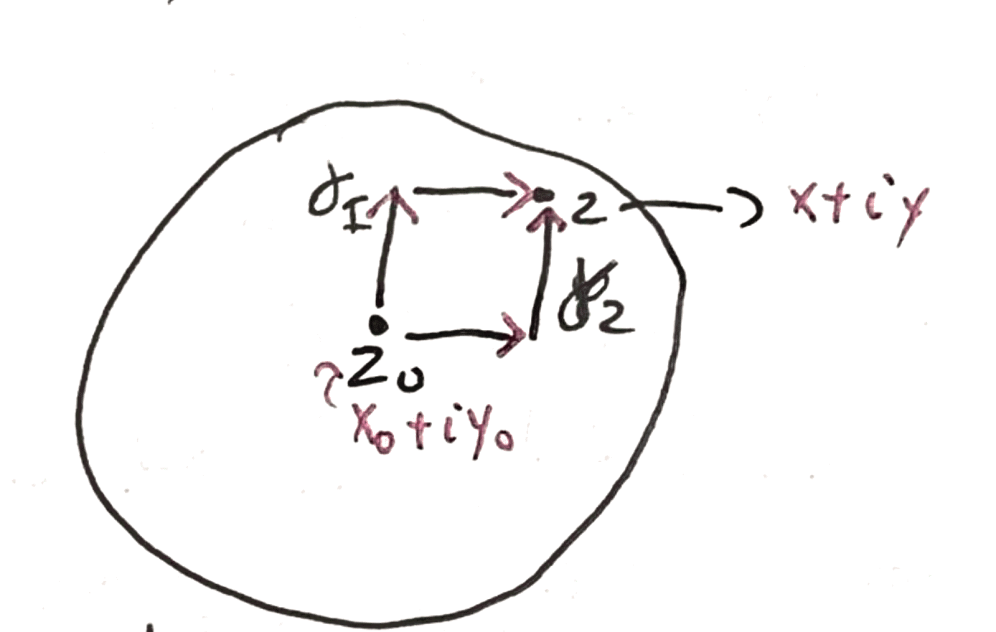
\includegraphics[width=.5\textwidth]{Figures/disk5.png}}\]
    For all $z \in \Omega$, define $F(z) = \int_{z_0}^z f(\xi) d\xi \coloneqq \int_{\gamma_1} f(z) dz = \int_{\gamma_2} f(z) dz$. We note that $F(z)$ is well-defined as Cauchy's Theorem guarantees the path-independence.\\\\
    \underline{We claim that $F \in CR^1(\Omega)$.} Indeed, tracing $\gamma_1$ and using the Fundamental Theorem of Calculus tells us that
    \[\frac{\partial F}{\partial x}(z) = f(z)\]
    Similarly, tracing along $\gamma_2$, we can parameterize $F(z)$ as
    \[F(z) = \int_{x_0}^x f(s + i y_0) ds + i \int_{y_0}^y f(x + it) dt\]
    Then it follows again that
    \[\frac{\partial F}{\partial y}(z) = i f(z)\]
    We can check that
    \[\frac{\partial F}{\partial x} + i \frac{\partial F}{\partial y} = f(z) - f(z) = 0\]
    , thus $F(z) \in CR^1(\Omega)$. Since $F(z)$ follows the Cauchy-Riemann Equations, we also know that
    \[F'(z) = \frac{1}{2}(\frac{\partial F}{\partial x} - i \frac{\partial F}{\partial y}) = \frac{1}{2}(2f(z)) = f(z)\]
    Since $F(z)$ is holomorphic, it is infinitely differentiable, so $f(z)$ is also holomorphic, so we are done.
\end{proof}

\begin{corollary}
    If $f_n \in C_z^1(\Omega)$ and $\{f_n\}$ converges to $f$ uniformly, then $f \in C_z^1(\Omega)$.
\end{corollary}

\begin{proof}
    For all sufficiently small rectangle $R$ within $\Omega$, consider
    \begin{align*}
        \int_{\partial R} f(z) dz &= \int_{\partial R} \lim_{n \to \infty} f_n dz\\
        &= \lim_{n \to \infty} \int_{\partial R} f_n dz \tag*{Uniform Convergence}\\
        &= \lim_{n \to \infty} 0 \tag*{Cauchy's Theorem}\\
        &= 0
    \end{align*}
    Thus, by Morera's Theorem, $f \in C_z^1(\Omega)$.
\end{proof}

\begin{corollary}
    If $f_n \in C_z^1(\Omega)$ and $\{f_n\}$ converges to $f$ uniformly, then $\{f_n'(z)\}$ converges to $f'(z)$ uniformly, and hence $\{f_n^{k}(z)\}$ converges to $f^{k}(z)$ uniformly.
\end{corollary}

\begin{proof}
It suffices for us to show this for the first derivative. Now for all $z \in \Omega$ and sufficiently small domain $G$, we have that
\begin{align*}
    f'(z) &= \frac{1}{2 \pi i} \int_{\partial G} \frac{f(z)}{(\xi - z)^2} d\xi \tag*{Cauchy's Formula for Derivatives}\\
    &= \frac{1}{2 \pi i} \int_{\partial G} \lim_{n \to \infty} \frac{f_n(z)}{(\xi - z)^2} d\xi\\
    &= \lim_{n \to \infty} \frac{1}{2 \pi i} \int_{\partial G} \frac{f_n(z)}{(\xi - z)^2} d\xi \tag*{Uniform Convergence}\\
    &= \lim_{n \to \infty} f_n'(z) \tag*{Cauchy's Formula for Derivatives}
\end{align*}
Thus, we have that $\{f_n'(z)\}$ converges to $f'(z)$. Since the original convergence is uniform, this convergence is also uniform.
\end{proof}

\begin{theorem}[Meta Theorem]
    Let $\phi(z, \xi): \Cbb \times X \to \Cbb$ where $X$ is some parameterization space with measure $\mu(\xi)$ that is finite, let
    $$f(z) = \int \phi(z, \xi) d\mu(\xi)$$
    Suppose $\phi$ is $CR^1$ in the variable $z$ and $f$ is bounded, then $f(z)$ is analytic.
\end{theorem}

\begin{proof}
    Since the measure $\mu$ is finite and the function is bounded, we can use Fubini's Theorem and see that, for all sufficiently small rectangles,
    \begin{align*}
        \int_R f(z) dz &= \int_R [\int \phi(z, \xi) d\mu(\xi)] dz\\
        &= \int [\int_R \phi(z, \xi) dz] d\mu(\xi) \tag*{Fubini's Theorem}\\
        &= \int 0 d\mu(\xi) \tag*{$\phi$ is $CR^1$ in the variable $z$}\\
        &= 0
    \end{align*}
\end{proof}

\begin{corollary}
    Let $f(z) = \sum_{n = 0}^\infty a_n (z - z_0)^n$ defined in $D_{z_0, r}$, then $f \in CR^1(D_{z_0, r}) = C_z^1(D_{z_0, r})$
\end{corollary}

\begin{proof}
    Let $z \in D(z_0, r)$, consider $r_1 > 0$ small enough that $cl(D(z, r_1)) \subset D(z_0, r)$, then by Heine-Cantor, we know that the partial sums
    \[\sum_{k = 0}^N a_k (z - z_0)^k \mapsto \sum_{0}^\infty a_n (z - z_0)^n \text{ converges uniformly in $D(z, r_1)$}\]
    Each of the partial sum are complex differentiable, thus by Corollary above, we have that $f \in C_z^1(D_{z_0, r})$.
\end{proof}

\begin{theorem}
    $CR^1 = C_z^1 = \text{Analytic}$
\end{theorem}

\begin{proof}
We have already shown all the directions in previous lectures and this lecture.
\end{proof}

\subsection{Power Series}

\begin{definition}
    Let $f(z) = \sum a_k (z - z_0)^k$ be a power series. We define the radius of convergence of $f$ as $R \in [0, \infty]$ such that for all $z$ such that $|z - z_0| < R$, $f(z)$ diverges, and for all $z$ such that $|z - z_0| > R$, $f(z)$ converges.
\end{definition}

\begin{remark}
    It turns out that
    \[\frac{1}{R} \coloneqq \lim \sup_{n \to \infty} |a_n|^{1/n}\]
\end{remark}

\begin{proposition}
    Let $f(z) = \sum a_k (z - z_0)^k$ be a power series with radius of convergence $R$, then $f(z)$ converges uniformly in any smaller disk of radius $r < R$ contained in $D_{z_0, R}$
\end{proposition}

\begin{proof}
    We note that $f$ is continuous on $D_{z_0, R}$, and the closure of any smaller disk is also contained in $D_{z_0, R}$, then apply Heine-Cantor.
\end{proof}

\begin{corollary}
    The following three power series:
    \begin{itemize}
        \item $\sum_{n = 0}^\infty a_n z^n$
        \item $\sum_{n = 0}^\infty n a_n z^{n-1}$
        \item $\sum_{n = 0}^\infty \frac{a_n}{n + 1} z^{n+1}$
    \end{itemize}
    all have the same radius of convergence.
\end{corollary}

\begin{proof}
    Exercise. Hint: Note that
    \[\lim_{n \to \infty} n^{1/n} = 1\]
\end{proof}

\begin{example}
    For sufficiently small $z \in \Cbb$, consider
    \[\frac{1}{1 + sin(z)} = 1 - sin(z) + sin^2(z) + ...\]
    , we can rewrite this into a power-series by noting that
    \[sin(z) = z - \frac{z^3}{3!} + \frac{z^5}{5!} + ...\]
\end{example}

\subsection{Liouville's Theorem}

\begin{theorem}
    Let $f \in Hol(\Cbb)$ be a holomorphic function on $\Cbb$, and for all $z \in \Cbb$ we have that $|f(z)| \leq M$ for some fixed $M \in \Cbb$, then $f(z)$ is identically constant.
\end{theorem}

\begin{proof}
Using Cauchy's Formula for Derivatives, we note that for all $z \in \Cbb$, for all $R > 0$,
\[f'(z) = \frac{1}{2\pi i} \int_{|\xi - z| = R} \frac{f(\xi)}{(\xi - z)^2} d\xi\]
Thus, we have that
\begin{align*}
    |f'(z)| \leq \frac{1}{2\pi} \max_{\xi \in |\xi - z|} |\frac{f(\xi)}{(\xi - z)^2}| \cdot 2 \pi R\\
    &\leq \frac{1}{2\pi} \frac{M}{R^2} \cdot 2 \pi R \tag*{Since $f$ is bounded}\\
    &= \frac{M}{R}
\end{align*}
Since this inequality holds for all $R > 0$, taking the limit as $R \to 0$, gives us that
\[|f'(z)| = 0\]
Hence $f'(z) = 0$, so
\[\frac{\partial f}{\partial z} = 0, \frac{\partial f}{\partial \overline{z}} = 0\]
So in other words
\[f_x - i f_y = 0, f_x + i f_y = 0 \implies f_x = 0, f_y = 0 \implies f(z) \text{ is constant}\]
\end{proof}

\begin{remark}
    While our Morera's Theorem applies to only triangles, up to a change of coordinate, the rectangle can really just be anything.
\end{remark}

\begin{remark}
    How to check say if $f(z) = |z|^2 = z \overline{z}$ is analytic or not? Well, we see that
    \[\frac{\partial f}{\partial \overline{z}} = \frac{\partial z}{\partial \overline{z}} \overline{z} + z \frac{\partial \overline{z}}{\partial \overline{z}} = 0 + z(1) \neq 0\]
    Thus, $f$ is not holomorphic and hence not analytic.\\\\
    Take another example, say $f(z) = |z| = (z \overline{z})^{1/2}$. This is real valued so we can use power rule and
    \[\overline{\partial}(f) = \frac{1}{2}(z \overline{z})^{-1/2} z \neq 0\]
\end{remark}

\subsection{Appendix - Cauchy–Hadamard Theorem}

In this section, we will discuss more about power series and convergence that was not covered during the lecture.

\begin{theorem}[Cauchy–Hadamard Theorem]
Consider $f(z) = \sum_{n = 0}^\infty a_n z^n$. Let $\frac{1}{0} = \infty$ and $\frac{1}{\infty} = 0$. Let $R$ be finite, non-zero, satisfying
\[\frac{1}{R} = \limsup |a_n|^{1/n}\]
Then $\sum_{n = 0}^\infty a_n z^n$ converges absolutely for $|z| < R$ and diverges for $|z| > R$. We call $R$ the \textbf{radius of convergence} and $|z| < R$ the \textbf{disc of convergence}.
\end{theorem}

% my attempt
\begin{proof}
For any $\epsilon > 0$, let $\rho \coloneqq \frac{1}{R}$.\\\\
If $|z| < R$, then there exist some $\epsilon > 0$ small enough that $|z| < \frac{1}{\rho + \epsilon} < \frac{1}{\rho} = R$. By the definition of $\limsup$ that for a sufficiently large $n$, for all $N > n$, 
\[|a_N|^{1/N} < \rho + \frac{\epsilon}{2} \ (*)\]
\begin{align*}
    |a_N z^N| &= |a_N^{1/N} z|^N\\
    &< |a_N^{1/N} \frac{1}{\rho + \epsilon}|^N \tag*{Since $|z| < \frac{1}{\rho + \epsilon}$}\\
    &< |\frac{\rho + \frac{\epsilon}{2}}{\rho + \epsilon}|^N \tag*{Using $(*)$}\\
\end{align*}
We note that $|\frac{\rho + \frac{\epsilon}{2}}{\rho + \epsilon}| < 1$ and $b_n = |\frac{\rho + \frac{\epsilon}{2}}{\rho + \epsilon}|^n$ forms a convergent geometric series. By the comparison test, we also have that $\sum_{n = N}^\infty a_n z^n$ converges, which implies that $\sum_{n = 0}^\infty a_n z^n$ converges.\\\\
If $|z| > R$, then there exist some $\epsilon > 0$ small enough that $|z| > \frac{1}{\rho - \epsilon} > \frac{1}{\rho} = R$. By the definition of $\limsup$ that for a sufficiently large $n$, for all $N > n$, 
\[|a_N|^{1/N} + \frac{\epsilon}{2} > \rho \ (*)\]
\begin{align*}
    |a_N z^N| &= |a_N^{1/N} z|^N\\
    &> |\frac{a_N^{1/N}}{\rho - \epsilon}|^N \tag*{Since $|z| > \frac{1}{\rho - \epsilon}$}\\
    &> |\frac{\rho - \frac{\epsilon}{2}}{\rho - \epsilon}|^N
\end{align*}
We note that $|\frac{\rho - \frac{\epsilon}{2}}{\rho - \epsilon}| > 1$ and $b_n = |\frac{\rho - \frac{\epsilon}{2}}{\rho - \epsilon}|^n$ forms a divergent geometric series, so the comparision test tells us that $\sum_{n = N}^\infty a_n z^n$ diverges, which implies that $\sum_{n = 0}^\infty a_n z^n$ diverges.
\end{proof}

\begin{corollary}\label{cor::radius_not_change}
Consider $f(z) = \sum_{n = 0}^\infty a_n z^n$ with radius of convergence $R > 0$, and let $g(z) = \sum_{n = 0}^\infty n a_n z^{n - 1}$. Then $g(z)$ has a radius of convergence that is also $R$.
\end{corollary}

\begin{proof}
Consider
\[\limsup_{n \to \infty} |n a_n|^{1/n} = \limsup_{n \to \infty} n^{1/n} |a_n^{1/n}|\]
It's a standard fact in real analysis that
\[\limsup_{n \to \infty} c_n b_n = \lim_{n \to \infty} c_n \limsup_{n \to \infty} b_n\]
if $\{c_n\}$ converges. We note that
\[\lim_{n \to \infty} n^{1/n} = 1\]
Since the limit exist
\[\limsup_{n \to \infty}  n^{1/n} |a_n^{1/n}| = \limsup_{n \to \infty} |a_n^{1/n}| = \frac{1}{R}\]
\end{proof}
\section{Lecture 6}

Previously, we have shown that a complex function $f: \Omega \to \Cbb$ is holomorphic if and only if it satisfies the Cauchy-Riemann Equations. Furthermore, if $f \in Hol(\Omega)$, $z_0 \in \Omega$, then we know $f$ is analytic and locally there exists some bounded, open set $G$ containing $z_0$ such that $\partial G$ is $PC^1$ $cl(G) \subset \Omega$, and on $G$,
\[f(z) = \sum_{k = 0}^\infty a_k (z - z_0)^k, |z - z_0| < r\]
\[a_n = \frac{1}{2 \pi i} \int_{\partial G} \frac{f(\xi)}{(\xi - z_0)^{n+1}} d\xi\]

\noindent Using the Cauchy's Formula for Derivatives, we note that
\[f^{(n)}(z_0) = \frac{n!}{2 \pi i} \int_{\partial G} \frac{f(\xi)}{(\xi - z_0)^{n+1}} d\xi \implies a_n = \frac{f^{(n)}(z_0)}{n!}\]

\subsection{Uniqueness Theorems}

\begin{theorem}
Let $f \in Hol(\Omega)$, $\Omega$ be an open and connected subset of $\Cbb$, and let $z_0 \in \Omega$ such that
\[f^{(n)}(z_0) = 0\ \forall n \geq 0\]
Then $f(z) = 0$ on $\Omega$, ie. $f$ is identically zero on $\Omega$.
\end{theorem}

\begin{proof}
We will prove this using \textbf{continuous induction}. Indeed, define $A$ to be the set
\[A \coloneqq \{z \in \Omega : f^{(n)}(z_0) = 0\ \forall n \geq 0\} = \bigcap_{n \geq 0} \{z \in \Omega: f^{(n)}(z) = 0\}\]
We first note that $A$ is closed since the preimage of $\{0\}$ is closed under continuous function and the intersection of closed sets are closed. Now clearly $A$ is non-empty, since $z_0 \in A$. We now \textbf{claim that $A$ is open}, then the connectedness of $\Omega$ would imply that $A = \Omega$.\\\\
Indeed, for all $z \in A$, since $f$ is holomorphic, we can find some $\epsilon(z) > 0$ small enough that locally
\[f(\xi) = \sum_{n = 0}^\infty \frac{f^{(n)}(z)}{n!}(\xi - z)^n, \forall \xi\ s.t.\ |\xi - z| < \epsilon\]
However, since $z \in A$, we know that
\[f(\xi) = \sum_{n = 0}^\infty \frac{0}{n!}(\xi - z)^n = 0\]
Thus we have that $\xi \in A$. Hence, $D_{z, \epsilon} \subset A$. Thus, $A$ is also open.
\end{proof}

\begin{remark}
The previous theorem shows that
\[f(z_0) = \sum a_n (z - z_0)^n, f^{(n)}(z_0) = 0\ \forall n \iff a_n = 0\ \forall n\]
\end{remark}

\begin{definition}[Limit Points]
Let $X$ be a topological space and $E \subset X$, we say $a \in X$ is a \textbf{accumulation/cluster/limit point} of $E$ if for all neighborhood $U$ containing $a$, $E \cap (U \setminus \{a\}) \neq \emptyset$
\end{definition}

\begin{theorem}[Uniqueness Theorem]\label{thm::uniqueness-theorem}
Let $f \in Hol(\Omega)$ where $\Omega$ is open and connected. Suppose $E \subset \Omega$ such that $f(z) = 0$ for all $z \in E$ and $E$ has some accumulation point $z_0$ in $\Omega$, then $f(z)$ is identically zero on $\Omega$.
\end{theorem}

\begin{proof}
The strategy is to apply the previous theorem. We first choose $r > 0$ small enough and consider the open disk $D_{z_0, r}$ to express $f$ as a power-series around $z_0$. Now, let $\Tilde{f}$ be $f$ restricted to $D_{z_0, r}$, we first claim that
\[\Tilde{f}(z_0) = 0\]
Indeed, since $z_0$ is a limit point of $E$, there exists a sequence of points $\{z_k\}$ in $E \cap D_{z_0, r}$ that converges to $z_0$. Since $f$ is continuous, we have that
\[\Tilde{f}(z_0) = \Tilde{f}(\lim_{k \to \infty} z_k) = \lim_{k \to \infty} \Tilde{f}(z_k) = \lim_{k \to \infty} 0 = 0\]
Now consider the power-series expression of $f$ around $z_0$:
\[[f(z) = \sum_{n = 0}^\infty a_n (z_0 - z)^n\]
Since $\Tilde{f}(z_0) = 0$, we clearly have that $a_0 = 0$. Now we will define
\[f_1(z) \coloneqq \frac{\Tilde{f}(z)}{z - z_0} = \sum_{n = 1}^\infty a_n (z - z_0)^{n-1}\]
\mattie{Division is fine here since $a_0 = 0$}
and define $\Tilde{f_1}(z)$ to be restricted to the same domain as before. Then clearly $f_1(z) = 0$ for all $z \in E \setminus \{z_0\}$, so it follows that $\Tilde{f_1}(z_0) = 0$, so $a_1 = 0$.\\\\
Using induction, we can conclude that all of the $a_n$ are $0$, so $f^{(n)}(z_0) = 0$ for all $n \geq 0$. Apply the previous result and we are done! 
\end{proof}

\begin{corollary}[Identity Theorem]
Let $f, g \in Hol(\Omega)$ where $\Omega$ is open and connected. Suppose $E \subset \Omega$ such that $f(z) = g(z)$ for all $z \in E$ and $E$ has some accumulation point $z_0$ in $\Omega$, then $f = g$ on $\Omega$.
\end{corollary}

\begin{proof}
Define $h(z) \coloneqq f(z) - g(z)$ and apply Theorem~\ref{thm::uniqueness-theorem}.
\end{proof}

\subsection{Analytic Extensions}

The uniqueness theorem implies that there's only one unique way to extend certain functions.

\begin{example}
Consider $f: \Rbb \to \Rbb$ given by $f(x) = e^x$, then $e^z = \sum_{n = 0}^\infty \frac{z^n}{n!}$ is an analytic extension of $e^x$ to the complex plane, and the identity theorem shows that it is in fact that only possible analytic extension.
\end{example}

\begin{proof}
Existence is already proven. For uniqueness, take $\Omega = \Cbb$ and $E = \Rbb$, $\Rbb$ clearly has an accumulation point in $\Cbb$, so we can apply the Identity Theorem.
\end{proof}

\begin{example}
Similarly, one can also show that
\[\cos(z) = 1 - \frac{z^2}{2!} + \frac{z^4}{4!} ...\]
\[\sin(z) = z - \frac{z^3}{3!} + \frac{z^5}{5!} ...\]
are the only unique extensions of $cos(x)$ and $sin(x)$, hence all trigonometric identities also hold for $z \in \Cbb$.
\end{example}

\begin{corollary}
Let $\Omega$ be an open connected set, suppose $f \in Hol(\Omega)$ isn't identically zero on $\Omega$, then the zeroes of $f$ are isolated.
\end{corollary}

\begin{proof}
Suppose not, then there exists a sequence of roots $\{z_k\}$ converging to some limit point. Then take $E = \{z_1, ..., z_k, ...\}$, then the Uniqueness Theorem tells us that $f$ is identically zero, so we have a contradiction.
\end{proof}

\begin{remark}
While this statement says that roots inside $\Omega$ are isolated, it says NOTHING about the boundary of $\Omega$.
\end{remark}

\subsection{Order of Zeroes}

\begin{definition}
Let $f \in Hol(\Omega)$, we define $Z(f)$ as the zero locus of $f$:
\[Z(f) \coloneqq f^{-1}(0)\]
\end{definition}

\begin{definition}
Suppose $f \in Hol(\Omega)$ and $f(z_0) = 0$, rewrite $f$ as a power series around $z_0$ as
\[f(z) = \sum_{n = 0}^\infty a_n (z - z_0)^n, a_0 = 0\]
We say the \textbf{order of zero} on $z_0$ is $\min \{n : a_n \neq 0\} = \min \{n: f^{(n)}(z_0) \neq 0$
\end{definition}

\begin{example}
$\sin(z)$ has zero of order $1$ at all roots. $(z - z_0)^3$ has a zero of order $3$ at $z_0$.
\end{example}
\section{Lecture 7}

\subsection{Revisiting Exponential}

\begin{definition}
    Let $z \in \Cbb$, we define the complex exponential map $e^z: \Cbb \to \Cbb$ as
    \[e^z \coloneqq 1 + z + \frac{z^2}{2!} + ... = \sum_{n = 0}^\infty \frac{z^n}{n!}\]
\end{definition}

\begin{theorem}[Euler's Identity]
Let $x \in \Rbb$, then
\[e^{ix} = cos(x) + i sin(x)\]
\end{theorem}

\begin{proof}
We can show this via explicit computation, indeed,
\begin{align*}
    e^{ix} &= \sum_{n = 0}^\infty \frac{(ix)^n}{n!}\\
    &= \sum_{k = 0}^\infty (-1)^k \frac{x^{2k}}{(2k)!} + i \sum_{k = 0} (-1)^k \frac{x^{2k + 1}}{(2k + 1)!} \tag*{Separate even and odd degree terms}\\
    &= cos(x) + i sin(x) \tag*{Taylor Series}
\end{align*}
\end{proof}

\begin{lemma}\label{lem::real_analy_fact}
Facts from Analysis:
\begin{enumerate}
    \item For every $r \in \Rbb$, $\sum_{n = 0}^\infty \frac{r^n}{n!}$ converges absolutely
    \item If $a_n \in \Cbb$ and $\sum_{n = 0}^\infty |a_n|$ converges, then $\sum_{n = 0}^\infty a_n$ converges
    \item If $L_a = \sum_{n = 0}^\infty a_n, L_b = \sum_{m = 0}^\infty b_m$ converges absolutely, then
    \[\sum_{n = 0}^\infty \sum_{k = 0}^n a_k b_{n - k}\]
    converges to
    \[(\sum_{n = 0}^\infty a_n) \cdot (\sum_{m = 0}^\infty b_m)\]
\end{enumerate}
This will helpful in proving some identities.
\end{lemma}

\begin{proof}
For $(1)$, we will use the ratio test. Indeed, consider $a_n = \frac{r^n}{n!}$, then
\[\lim_{n \to \infty} |\frac{a_{n+1}}{a_n}| = \lim_{n \to \infty} |\frac{r}{n + 1}| = 0 < 1\]
Thus, the series converges absolutely.\\\\
For $(2)$, let $b_n = \sum_{i = 1}^n a_i, c_n = \sum_{i = 1}^n |a_i|$. We note that the topology $\Cbb$ is homeomorphic to the Euclidean topology on $\Rbb^2$, so in particular $\Cbb$ is a complete metric space, so a sequence is convergent if and only if it is Cauchy. We know $c_n$ converges, so for every $\epsilon > 0$, there exists some $N_c$ such that for all $i, j > N_c$.
\[|c_i - c_j| < \epsilon\]
It remains for us to show that $b_n$ is also Cauchy. Indeed, if $i = j$, then we are done. Without loss, we will then assume $j > i$, then
\begin{align*}
    |b_i - b_j| &= |\sum_{k = i + 1}^j a_k|\\
    &\leq \sum_{k = i + 1}^j |a_k| \tag*{Triangle's Inequality}\\
    &= |c_i - c_j|\\
    &< \epsilon
\end{align*}
Thus, $\{b_n\}$ is Cauchy and converges.\\\\
For $(3)$, $(\sum_{n = 0}^\infty a_n) \cdot (\sum_{m = 0}^\infty b_m)$ certainly converges to $L_a \cdot L_b$. Now write $(\sum_{n = 0}^\infty a_n) \cdot (\sum_{m = 0}^\infty b_m) = \sum_{n = 0}^\infty \sum_{m = 0}^\infty a_n b_m$, this corresponds exactly to the terms of $\sum_{n = 0}^\infty \sum_{k = 0}^n a_k b_{n - k}$. The exact combinatorics is left as details to the reader.
\end{proof}

\begin{corollary}
Let $e^z$ be the complex exponential map, then
\begin{itemize}
    \item $e^z$ converges for all $z \in \Cbb$
    \item $e^{z + w} = e^z \cdot e^w$ for all $z, w \in \Cbb$
\end{itemize}
\end{corollary}

\begin{proof}
For the first, let $a_n = \sum_{k = 1}^n |\frac{z^k}{k!}|$. It suffices for us to prove that $a_n$ converges as absolute convergence implies monotone convergence from Lemma~\ref{lem::real_analy_fact}(2). But we note that 
\[|\frac{z^k}{k!}| = \frac{|z|^k}{k!}\]
and $|z|$ is a real number, so Lemma~\ref{lem::real_analy_fact}(1) tells us that $a_n$ converges.\\\\
For the second, we note that
\begin{align*}
    e^{z + w} &= \sum_{n = 0}^\infty \frac{(z + w)^n}{n!}\\
    &= \sum_{n = 0}^\infty \sum_{k = 0}^n {n \choose k} \frac{z^k w^{n-k}}{n!} \tag*{Binomial Theorem}\\
    &= \sum_{n = 0}^\infty \sum_{k = 0}^n \frac{z^k}{k!} \frac{w^{n-k}}{(n - k)!}\\
    &= (\sum_{n = 0}^\infty \frac{(z)^n}{n!}) \cdot (\sum_{n = 0}^\infty \frac{(w)^n}{n!}) \tag*{By Lemma~\ref{lem::real_analy_fact}(3)}\\
    &= e^z \cdot e^w
\end{align*}
\end{proof}

\begin{proposition}
We can also recover $\cos(z)$ and $\sin(z)$ from $e^z$ as
\[\cos(z) = \frac{e^{iz} + e^{-iz}}{2}, \sin(z) = \frac{e^{iz} - e^{-iz}}{2i}\]
If $x \in \Rbb$, we also have that
\[\cos(x) = \Re e^{ix}, \sin(x) = \Im e^{ix}\]
\end{proposition}

\subsection{Complex Logarithms}

As in the case of $\Rbb$, we want to define $\log(z)$ as an inverse to $e^z$ such that
\[e^{\log(z)} = z\]
The problem is that $e^z$ is not actually injective, so there are multiple choices for $\log(z)$. Consequently, this will result in $\log(z)$ not being continuous on all of $\Cbb$.

\begin{question}
Given $z$, can we find all solutions satifying $e^w = z$?
\end{question}

\begin{proof}[Answer]
We will again leverage on Polar Coordinates. Indeed, write $z = re^{i \theta}, w = x + iy$, then we have that
\[r e^{i \theta} = e^{x + iy} = e^{x} e^{iy}\]
Thus, $x = \log(r), y = \theta + 2 \pi k$.\\\\
Thus, $w$ is of the form $w_k = \log(r) + i(\theta + 2 \pi k)$
\end{proof}

\begin{definition}[Complex Logarithm]
    For $z \in \Cbb \setminus \{0\}$, write $z = re^{i \theta}, \theta \in [-\pi, \pi]$. Then we define
    \[\log(z) = \log(r e^{i \theta}) \coloneqq \log(r) + i \theta\]
    $\theta$ is sometimes refered to as the \textbf{principal argument} of $z$ and we denote $Arg(z) = \theta$.
\end{definition}

\begin{remark}
Note that the complex logarithm $\log(z)$ is not continuous on all of $\Cbb$:
\[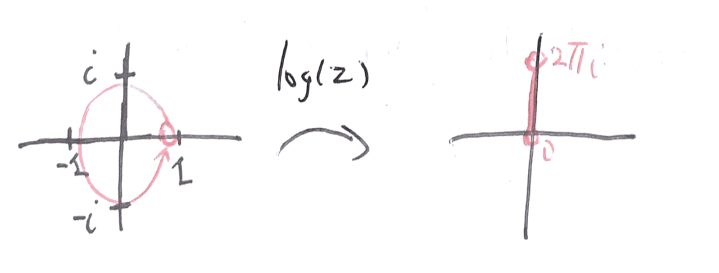
\includegraphics[width=0.5\textwidth]{Figures/complex_log.png}\]
As you trace around the unit circle, going back to $z = 1$ presents a problem.\\\\
Therefore, we can only define the complex logarithm up to a \textbf{branch cut} that's a radial line extending out from the origin. We will without loss choose this branch to be $(-\infty, 0]$
\end{remark}

\begin{proposition}
$\log(z)$ is holomorphic on $\Cbb \setminus (-\infty, 0]$ and in fact $\frac{d}{dz} \log(w) = \frac{1}{w}$
\end{proposition}

\begin{proof}
One way to do this is to use the Cauchy-Riemann equations in polar coordinates. We will however use the Inverse Function Theorem instead. Indeed, we note that on $\Cbb \setminus (-\infty, 0]$, $z \mapsto e^z$, when viewed as a function from $\Rbb^2$ to $\Rbb^2$, is a smooth function whose derivative is exactly
\[(e^z)' = e^x \begin{pmatrix} cos(y) & -sin(y)\\ sin(y) & cos(y) \end{pmatrix}\]
, which satisfies the matrix representation of complex numbers (hence we can extend the argument to holomorphic functions). Thus, the inverse function theorem tells us that $g(z) = \log(z)$ is also holomorphic and that
\[g'(f(x)) = (f'(x))^{-1}\]
This equation tells us that, locally for all $w = e^z \in \Cbb \setminus (-\infty, 0]$,
\[\frac{d}{dz} \log(w) = e^{-x}\begin{pmatrix} cos(y) & sin(y)\\ -sin(y) & cos(y) \end{pmatrix} = (e^{z})^{-1} = \frac{1}{w}\]
Note that the branch cut does not prevent the existence of a local inverse, but it does prevent the existence of a global inverse on all of $\Cbb$.
\end{proof}

\begin{remark}
Let $z \in \Cbb \setminus (-\infty, 0]$, then since $\frac{1}{z}$ is primitive on the path $1$ to $z$, we have that:
\[\int_1^z \frac{d\xi}{\xi} = \log(z) - \log(1) = \log(z)\]
\end{remark}

\subsection{Homotopy Invariance of Integral}

Let $f \in Hol(\Omega)$ and $\gamma: [a, b] \to \Gamma$ is continous and $\Gamma \subset \Omega$, then we can define the integral
\[\int_\gamma f(z) dz\]

Informally, we can define this because at each point on $\gamma$, we can find some disk to represent $f$ as a power series with a primitive $F$, then we can split $[a, b]$ into a union of (not necessarily uniform) subintervals, then the integral $\gamma$ can be approximated as a sum of the anti-derivatives $F_k$ at each end-points.

We can formally justify this with what's called the Lebesgue's Number Lemma.

\begin{lemma}[Lebesgue's Number Lemma]
Let $K$ be a compact metric space and let $\{U_a\}$ be an open cover for $K$, then there exists some $\delta > 0$ (we call the \textbf{Lebesgue Number}) such that for all $x \in K$, there exists some $a$ such that $B_{x, \delta} \subset U_a$
\end{lemma}

\begin{proof}
For all $x \in K$, since $\{U_a\}$ is an open cover of $K$, there exists some $a$ such that $x \in U_a$. Since $U_a$ is open, there exists some $r(x) > 0$ small enough such that $B_{x, 2r(x)} \subset U_\alpha$.\\\\
Note that $\{B_{x, r(x)}\}$ running over all $x \in K$ is an open cover of $K$. Since $K$ is compact, we in fact have a finite subcover:
\[B_{x_1, r_1}, ..., B_{x_n, r_n}\]
Choose $\delta = \min \{r_i\}$. Now for all $x \in K$, it belongs to one of the $B_{x_k, r_k} \subset U_a$.\\\
Then we claim $x \in B_{x, \delta} \subset B_{x_k, 2r_k} \subset U_a$. To do this, we need to verify $B_{x, \delta} \subset B_{x_k, 2r_k}$. Indeed, for all $y \in B_{x, \delta}$, we have that
\[d(y, x_k) \leq d(y, x) + d(x, x_k) < \delta + r_k \leq 2r_k\]
This concludes the proof.
\end{proof}

To apply this lemma in our context, we take $K = [a, b]$ and for all $s \in [a, b]$, we define $U_s = \gamma^{-1}(D_{\gamma(s), r(s)})$, where $r(s)$ is the radius of convergence of $\gamma(s)$ under the power-series. Then we can apply the Lebesgue's Number Lemma.

\begin{question}
Is the integral well-defined up to two different splitting?
\end{question}

\begin{proof}[Answer]
Yes, the idea is that given two splitting on the interval, one can join them using a refinement by taking smaller intervaks of both of them and used the associated anti-derivative from either original splittings. To be more rigorous, let $\{I_k\}$ and $\{J_n\}$ be two different splittings of the interval $[0, 1]$. Now define
\[I_{k, n} \coloneqq I_k \cap J_n\]
Then we note that, by definition, the integral over the splitting $I_{k, n}$ would be of the form
\begin{align*}
    \sum \int_{I_{k, n}} f(z) dz &= \sum_{k} \sum_{n} \int_{I_{k, n}} f(z) dz\\
    &= \sum_k [\sum_{n} \int_{I_{k, n}} f(z) dz]\\
    &= \sum_k \int_{I_k} f(z) dz
\end{align*}
Similarly, we can also show that
\[\sum \int_{I_{k, n}} f(z) dz = \sum_n \int_{J_n} f(z) dz\]
Thus, the two splittings yield the same integral.
\end{proof}

\begin{definition}
    Let $\gamma_0, \gamma_1: [a, b] \to \Omega$ be continuous. We say $\gamma_0$ is \textbf{homotopy equivalent} to $\gamma_1$ if there exists a continuous function $\Gamma: [a, b] \times [0, 1] \to \Omega$ such that $\Gamma(s, 0) = \gamma_0(s)$ and $\gamma(s, 1) = \gamma_1(s)$ for all $s \in [a, b]$.\\
    We will also assume that either:
        \begin{itemize}
            \item All pathes are closed, for all $t$
            \[\Gamma(a, t) = \Gamma(b, t)\]
            \item OR Endpoints are fixed
            \[\Gamma(a, t) = \gamma_0(a) = \gamma_1(b)\]
            \[\Gamma(b, t) = \gamma_0(b) = \gamma_1(b)\]
        \end{itemize}
\end{definition}

\begin{theorem}
If $\gamma_0, \gamma_1$ are homotopy equivalent in $\Omega$ and $f \in Hol(\Omega)$, then
\[\int_{\gamma_0} f(z) dz = \int_{\gamma_1} f(z) dz\]
\end{theorem}

\begin{remark}
In a simply connected domain, any two pathes are homotopy equivalent. In otherwords, the path of integration is irrelevant.
\end{remark}
\section{Lecture 8}

\subsection{Homotopy Invariance of Integrals - Continued}

\begin{theorem}
If $\gamma_0, \gamma_1$ are homotopy equivalent in $\Omega$ and $f \in Hol(\Omega)$, then
\[\int_{\gamma_0} f(z) dz = \int_{\gamma_1} f(z) dz\]
\end{theorem}

\begin{proof}
Let $\Gamma$ be the homotopy equivalence function. For all $z_0 \in \Omega$, let $D_{z_0}$ be a disc centered at $z_0$ small enough such that $f$ can be expressed as a power-series on it, define
\[U_{z_0} = \Gamma^{-1}(D_{z_0})\]
Then $\{U_{z_0}\}$ will be an open cover of $R \coloneqq [a, b] \times [0, 1]$, which is a compact metric space. Apply Lebesgue's Number Lemma, we find $\delta > 0$ such that, we can split $R$ into smaller rectangles $R_k$ where each $diam(R_k) < \delta$.\\\\
The Lebesgue Number Lemma tells us that, for each $R_k$, $\Gamma(cl(R_k)) \subset D_{z}$ for some $z$. Since $f$ is primitive on $D_z$, we have that
\[\int_{\Gamma|_{\partial R_k}} f(z) dz = 0\]
Putting the small rectangles together (Green's Theorem style), the inner edges cancel out, so we have that
\[\int_{\Gamma|_{\partial R}} f(z) dz = 0\]
Now consider the pathes $\ell_1 = \{a\} \times [0, 1]$ and $\ell_2 = \{b\} \times [0, 1]$, we claim that
\[\int_{\Gamma|_{\ell_1 + \ell_2}} f(z) dz = 0\]
Indeed, if endpoints are fixed, both paths are constant (stays at same point). If all path are closed, then this is the same path in opposite directions.\\\\
Thus, we only have to integrate over the horizontal pathes:
\[\int_{\partial R} f(z) dz = 0 = \int_{\gamma_0} f(z) dz - \int_{\gamma_1} f(z) dz\]
\end{proof}

\begin{definition}
    A set $\Omega$ is \textbf{simply connected} if any closed loop in $\Omega$ is homotopy equivalent to the constant path. This is equivalent to saying, for any pathes $\gamma_0, \gamma_1$, $\gamma_0(a) = \gamma_1(a) = z_0$, $\gamma_0(b) = \gamma_1(b) = z_1$, are homotopy equivalent.
\end{definition}

\begin{remark}
If $\Omega$ is simply connected domain, then
\[\int_{z_0}^z_1 f(z) dz\]
does not depend on the path specified.
\end{remark}

\begin{definition}
    Let $\Omega$ be simply connected and $f \in Hol(\Omega)$. Suppose $f(z) \neq 0$ for all $z \in \Omega$.\\\\
    Fix some $z_0 \in \Omega$, and consider
    \[a_0 \text{ such that } f(z_0) = e^{a_0}\]
    We can find $a_0$ as
    \[Re(a_0) = \log |f(z_0)|, Im(a_0) = arg\ f(z_0)\]
    Then we define
    \[\log f(z) \coloneqq a_0 + \int_{z_0}^z \frac{f'(\xi)}{f(\xi)} d\xi\]
\end{definition}

Show that $\log f(z)$ aligns with the global definition of the complex logarithm.

\begin{proof}
Exercise. The idea is to denote $\varphi(z) = a_0 + \int_{z_0}^z \frac{f'(\xi)}{f(\xi)} d\xi$ and show that
\[(f(z) e^{-y(z)})' = 0\]
and realize that their product must be $1$.
\end{proof}

\mattie{explain motivation later}
\begin{definition}
    What is $f(z)^{\alpha}$? We define
    \[f(z)^{\alpha} = e^{\alpha \log(f(z))}\]
    This is defined when $f \in Hol(\Omega)$, $f(z) \neq 0$ on all of $\Omega$, and $\Omega$ is simply connected.
\end{definition}

In a simply connected domain, the branch of the logarithm, it is enough to be determined by which $a_0$ you choose.

\subsection{Laurent Series}

Suppose $f$ is holomorphic on $\{z : a < |z - z_0| < A\}$, where we require $a \geq 0$ and $A \leq \infty$.

\begin{theorem}
If $f \in Hol\{z : a < |z - z_0| < A\}$, then $f$ can be represented as
\[f(z) = \sum_{n \in \Zbb} a_n (z - z_0)^n\]
, where we have that
\[a_n = \frac{1}{2\pi i} \int_{|\xi - z_0| = r} f(\xi) (\xi - z_0)^{-(n+1)} d\xi\]
, where $r$ is between $a < r < A$ (Note that for $\Zbb_+$, this is the same as the Taylor Power Series)
\end{theorem}

\begin{proof}
Without loss of generality, we can shift this to $z_0 = 0$.\\\\
Take $z$ such that $a < |z| < A$ and pick $r, R$ such that
\[a < r < |z| < R < A\]
Then consider the set
\[G \coloneqq \{z: r < |z| < R \}\]
Then Cauchy's Integral Formula gives
\begin{align*}
    f(z) &= \frac{1}{2\pi i} \int_{\partial G} \frac{f(\xi)}{\xi - z} d\xi\\
    &= \frac{1}{2\pi i} (\int_{|z| = R} \frac{f(\xi)}{\xi - z} d\xi - \int_{|z| = r} \frac{f(\xi)}{\xi - z} d\xi)\\
    &= \frac{1}{2\pi i} (I_1 - I_2)
\end{align*}
For $I_1$, we note that $|z| < |\xi| = R$, so
\begin{align*}
    I_1 &= \int_{|z| = R} \frac{f(\xi)}{\xi - z} d\xi\\
    &= \int_{|z| = R} \frac{f(\xi)}{\xi} \frac{1}{1 - \frac{z}{\xi}} d\xi\\
    &= \int_{|z| = R} f(\xi) \sum_{k = 0}^\infty \frac{z^k}{\xi^{k+1}}
\end{align*}
For $I_2$, we note that $|z| > |\xi| = r$, so
\begin{align*}
    I_2 &= \int_{|z| = r} \frac{f(\xi)}{\xi - z} d\xi\\
    &= \int_{|z| = r} \frac{-f(\xi)}{z} \frac{1}{1 - \frac{\xi}{z}} d\xi\\
    &= \int_{|z| = r} -f(\xi) \sum_{k = 0}^\infty \frac{\xi^k}{z^{k+1}}\\
    &= \int_{|z| = r} -f(\xi) \sum_{n = -\infty}^{-1} \frac{z^n}{\xi^{n+1}}\\ \tag*{Change of Variables}
\end{align*}
Since both series converge uniformly, we can integrate term by term and use Cauchy's Formula for Derivatives, rewriting both $I_1$ and $I_2$ out in series finishes the proof.
\end{proof}

Now we will consider a particular case of the Laurent Series!

\begin{definition}
    Let $f \in Hol(\Omega \setminus \{z_0\})$ where $z_0 \in \Omega$. In this case, we say $f$ has a singularity at $z_0$.\\\\
    Take $\delta$ small enough and $D_{z_0, \delta} \subset \Omega$, then the Laurent Series tells us
    \[f(z) = \sum_{n \in \Zbb} a_n (z - z_0)^n\]
    We say that
    \begin{itemize}
        \item $f$ has a \textbf{removable singularity} at $z_0$ if $a_n = 0$ for all $n < 0$. In this case,
        \[f(z) = \sum_{n \geq 0} a_n (z - z_0)^n, f(z_0) = a_0\]
        An example of such function would be $f(z) = \frac{sin(z)}{z}$ has removable singularity at $0$
        \item We say $f$ has a \textbf{pole at $z_0$} if $a_n \neq 0$ for finitely many $n < 0$. We say the \textbf{order of a pole} as
        \[\max \{n \geq 0: a_{-n} = 0\}\]
        \item We say that $f$ has an essential singularity if there exists infinitely many $n < 0$ such that $a_n \neq 0$.\\\\
        For example consider
        \[f(z) = e^{1/z} = \sum_{n = 0}^\infty \frac{z^{-n}}{n!}\]
        This has an essential singularity at $z = 0$.
    \end{itemize}
    These are the singularities we care about.
\end{definition}
\section{Lecture 9}

\subsection{Classification of Singularities}

Recall, let $f \in Hol(\Omega \setminus \{z_0\})$, where $z_0 \in \Omega$, we can write $f$ into a Laurent series
\[f(z) = \sum_{z \in \Zbb} a_n (z - z_0)^n, 0 < |z - z_0| < N\]
, and we say that $z_0$ is removable if $a_n = 0$ for all $n < 0$.

\begin{theorem}
$z_0$ is a removable singularity of $f$ if and only if there exists a neighborhood $z_0 \in U$ such that $f$ is bounded in $U \setminus \{z_0\}$.
\end{theorem}

\begin{proof}
If $f$ has a removable singularity, we can write it locally as
\[f(z) = \sum_{n \geq 0} a_n (z - z_0)^n\]
which has a positive radius of convergence and hence bounded in a neighborhood of $z_0$.\\\\
Conversely, suppose $f$ is bounded on $0 < |z - z_0| < \delta$. Then for all $n \geq 1$, we note that
\[a_{-n} = \frac{1}{2\pi i} \int_{|z - z_0| = r} f(z) (z - z_0)^{n-1} dz \]
As $n-1 \geq 0$ and $f$ is bounded, this integral is also bounded, so
\[|a_{-n}| \leq \frac{1}{2\pi} M (1) (2\pi r) = Mr\]
for all $0 < r < \delta$, we can shrink $r$ down and have that $a_{-n} = 0$.
\end{proof}

\begin{remark}
If $f(z) = o(\frac{1}{|z - z_0|})$, then $f$ has a removable singularity at $z_0$.
\end{remark}

We say $f$ has a \textbf{pole at $z_0$} if $a_n \neq 0$ for finitely many $n < 0$. We say the \textbf{order of a pole} as
        \[\max \{n \geq 0: a_{-n} = 0\}\]
        
\begin{theorem}
$z_0$ is a pole if and only if $\lim_{z \to z_0} |f(z)| = \infty$
\end{theorem}

\begin{proof}
Suppose $z_0$ is a pole of order $m$, then we can write
\[f(z) = \frac{g(z)}{(z - z_0)^m}, g(z_0) \neq 0\]
Hence we have that
\[\lim_{z \to z_0} |f(z)| = \lim_{z \to z_0} |\frac{g(z)}{(z - z_0)^m}| = \infty\]
Conversely, suppose $\lim_{z \to z_0} |f(z)| = \infty$, then we can find some $r > 0$ such that $|f(z)| > 1$ for all $z$ in $0 < |z - z_0| < r$.\\\\
Now consider $h(z) = \frac{1}{f(z)}$ on $D_{z_0, r} \setminus \{z_0\}$, then $h(z) \in Hol(D_{z_0, r} \setminus \{z_0\})$ and $\lim_{z \to z_0} h(z) = 0$ - so we can extend $h$ to the whole disk. Therefore it has to be the case that $|h(z)| < 1$, then by the previous theorem, this means $z_0$ is a removable singularity for $h$, so in fact $h$ is holomorphic on the whole disk.\\\\
Since $h(z_0) = 0$, we can find the smallest $m$ such that $h(z) = (z - z_0)^m h_0(z)$ but $h_0(z_0) \neq 0$. Now consider $g = \frac{1}{h}$, then we have that
\[f(z) = \frac{g(z)}{(z - z_0)^m}\]
Thus, $z_0$ is a pole of order $m$.
\end{proof}

We say that $f$ has an essential singularity if there exists infinitely many $n < 0$ such that $a_n \neq 0$.

\begin{theorem}[Casorati-Weierstrass Theorem]
If $f$ has an essential singularity at $z_0$, then for any neighborhood $U$ of $z_0$, $U \subset \Omega$, $f(U)$ is \textbf{dense} in $\Cbb$ (in other words, for all $w \in \Cbb$, there exists a sequence of $z_n$ such that $f(z_n) \to w$ as $z_n \to z_0$)
\end{theorem}

\begin{proof}
We will prove this using contradiction. Suppose there exists some neighborhood $U$ of $z_0$ such that $f(U)$ is not dense. Then there exists some $a \in \Cbb$ and $r > 0$ such that $D_{a, r} \cap f(U) = \emptyset$.\\\\
Now define $g(z) = \frac{1}{f(z) - a}$. Then clearly $g \in Hol(U)$ as the denominator is never $0$. We also have that $|g| < \frac{1}{|f(z) - a|} < \frac{1}{r}$. Moreover, we note that $g(z) \neq 0$ in $U \setminus \{z_0\}$ because $f$ is bounded. While $g(z_0)$ could be $0$, we will choose the smallest $m$ such that $g(z) = (z - z_0)^m g_0(z)$ and $g_0(z_0) \neq 0$.\\\\
Thus, $g_0(z) \neq 0$ on $U$. But we have that
\[f(z) = \frac{1}{g(z)} + a = \frac{1}{(z - z_0)^m g_0(z)} + a\]
, so $f$ has a removable singularity or some pole at $z_0$, hence a contradiction.
\end{proof}

\begin{definition}
    Suppose $f$ has a singularity at $z_0$ and write
    \[f(z) = \sum_{n \in \Zbb} a_n (z - z_0)^n\]
    Then we define the \textbf{residue of $f$ at $z_0$} as $a_{-1}$ and denote is as $Res_{z_0}(f)$ or $res(f, z_0)$
\end{definition}

\begin{remark}
If $z_0$ is a pole of order $1$, then
\[res(f, z_0) = \lim_{z \to z_0} (z - z_0)f(z)\]
\end{remark}

\subsection{Cauchy's Residue Theorem}

\begin{theorem}[Cauchy's Residue Theorem]
Let $G$ be a bounded domain with $\partial G \in PC^1$ and $\overline{G} \subset \Omega$. Let $z_1, ..., z_n \in G$ and $f \in Hol(\Omega \setminus \{z_1, ..., z_n\})$, then
\[\int_{\partial G} f(z) dz = 2\pi i \sum_{k = 1}^n Res(f, z_k)\]
\end{theorem}

\begin{proof}
Let $D_k$ be small disks around each $z_k$ and consider $\Tilde{G} = G \setminus \bigcup D_k$. Note that $f(z)$ is holomorphic on $\Tilde{G}$, so
\[\partial_{\partial \Tilde{G}} f(z) dz = 0\]
On the other hand, we also have that $\partial \Tilde{G} = \partial G - \bigcup \partial D_k$, so in other words
\[\int_{\partial G} f(z) dz = \sum_k \int_{\partial D_k} f(z) dz\]
Write $f$ as a Laurent Series, then every term except for the $-1$ term is primitive and thus evaluate to $0$, so we are left with:
\[\int_{\partial G} f(z) dz = 2\pi i \sum_{k = 1}^n Res(f, z_k)\]
\end{proof}
\section{Lecture 10 - 09/28/2022}

Clarification from last lecture: In the proof of the Casorati–Weierstrass theorem, we have that $g(z) \neq 0$ for all $z \in U\setminus \{z_0\}$, but $g(z_0) = 0$ is totally possible! Hence we write
\[f(z) = \frac{1}{g(z)} + a\]
, where $f$ either has a pole or a removable singularity at $z_0$, giving the contradiction.

\subsection{Computing Real Integrals with Residues}

\begin{example}[A Straight-forward Application]
Let $s \in \Rbb$, consider the integral
\[I = \int_{-\infty}^\infty \frac{1}{x^2 + 1} e^{isx} dx\]
Let $f(z) = \frac{1}{x^2 + 1} e^{isx}$, then $I = \int_{\Rbb} f(z) dz = \pi e^{-|s|}$
\end{example}

\begin{remark}
Why do we even care about integrals of this form? Well, they are really closed aligned with \textbf{inverse Fourier transforms}. In particular, you would calculate integrals of the form
\[F(s) = \int_{-\infty}^\infty f(x) e^{-2\pi i s} dx\]
\end{remark}

\begin{proof}[Proof of Example]
We will consider three cases $s = 0, s > 0,$ and $s < 0$. For $s = 0$, this is obvious.\\\\
Now for $s > 0$, consider the following contour:
\[\fbox{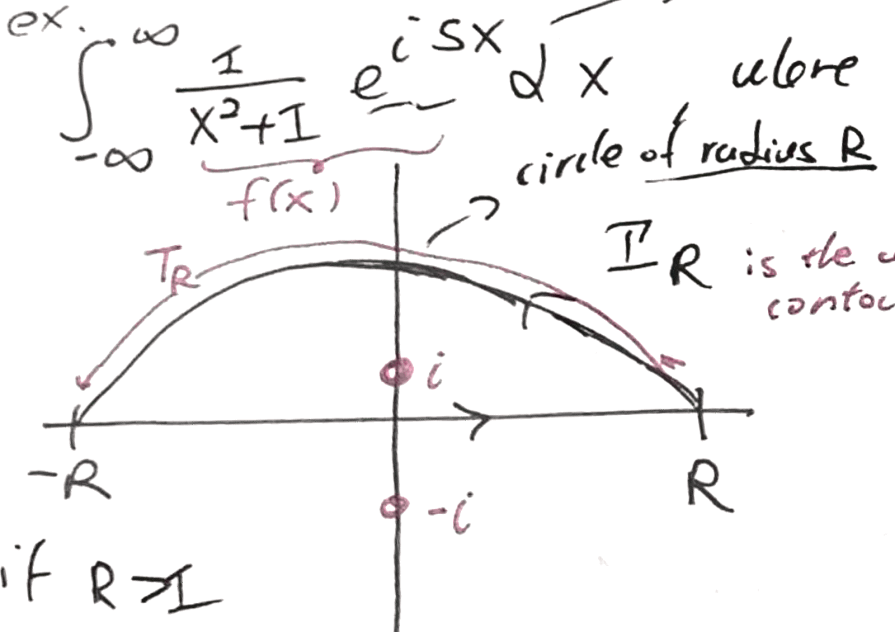
\includegraphics[width=.5\textwidth]{Figures/contour-1.png}}\]
Then Cauchy's Residue Theorem tells us that
\[\int_{\Gamma_R} f(z) dz = 2 \pi i Res(f, i)\]
$i$ is a pole of order $1$ for $f$, so
\[Res(f, i) = \lim_{z \to i} (z -i)f(z) = \frac{e^{-s}}{2i}\]
Thus, we have that
\[\int_{\Gamma_R} f(z) dz = \pi e^{-s}\]
Now take $R \to \infty$, we note that since \textbf{$f$ is integrable} as $\int_{-\infty}^\infty |f(x)| dx < \infty$,
\[\lim_{R \to \infty} \int_{-R}^R f(z) dz = \int_{-\infty}^{\infty} f(z) dz = I\]
So in other words,
\[I = \lim_{R \to \infty} [\int_{\Gamma_R} f(z) dz - \int_{T_R} f(z) dz] = \pi e^{-s} - \lim_{R \to \infty} \int_{T_R} f(z) dz\]
We want to show that the last term goes to $0$, indeed
\begin{align*}
    \int_{T_R} f(z) dz &= \int_0^\pi \frac{e^{isRe^{it}}}{(Re^{it})^2 + 1} i Re^{it} dt \tag*{Let $z = R e^{it}$}\\
    |\int_{T_R} f(z) dz| &\leq \frac{R}{R^2 - 1} \pi \tag*{Note that $e^{isRe^{it}}$ is bounded by $1$ as $s > 0$ and $0 < t < \pi$}
\end{align*}
Taking $R \to \infty$, the bound goes to $0$, thus, we have that
\[I = \pi e^{-s}, s \geq 0\]
\textbf{What about when $s < 0$}? In this case, $\int_{T_R} f(z) dz$ would not actually go to $0$, so instead, we need to consider the opposite contour:
\[\fbox{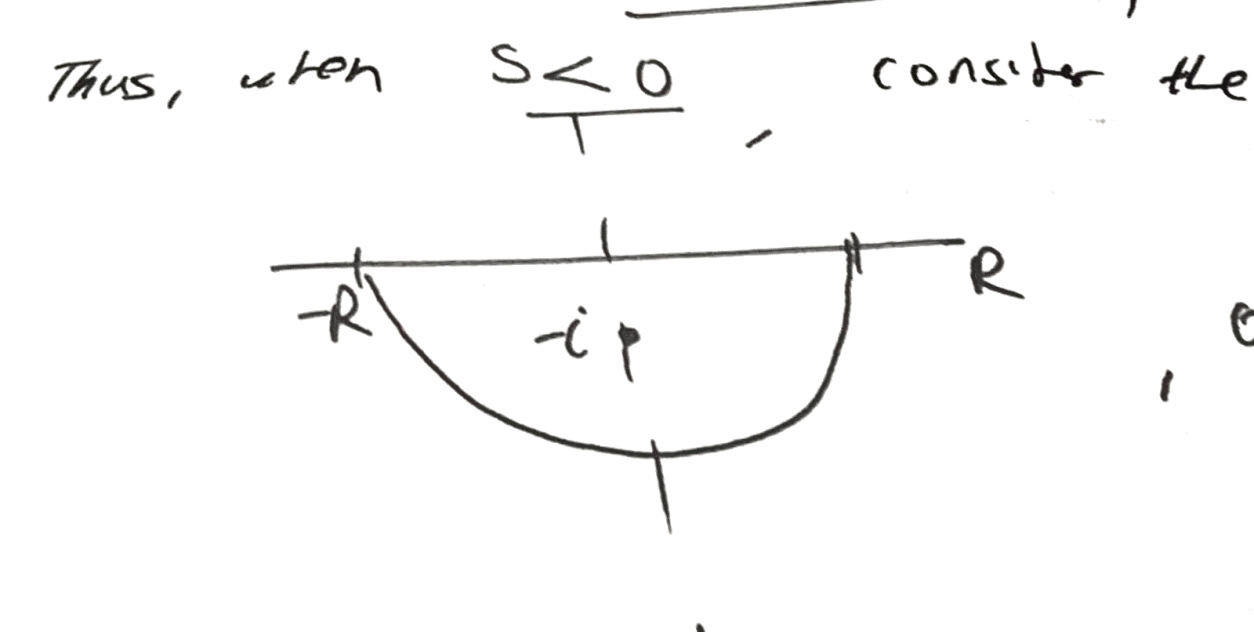
\includegraphics[width=.5\textwidth]{Figures/contour-2.png}}\]
, and we can similarly show the result is true. Alternatively, we could also have argued using symmetry.\\\\
Note that while we proved this using a circle, we could have also used a rectangle instead.
\end{proof}

\begin{example}[A Not-So-Simple Application]
Let $s \in \Rbb$ and $a \in \Cbb$ such that $s > 0$ and $\Im(a) > 0$, consider the integral
\[I = \int_{-\infty}^\infty \frac{e^{isx}}{x - a} dx\]
Let $f(z) = \frac{e^{isz}}{z - a}$, then what is $I$?
\end{example}

Consider the following contour:
\[\fbox{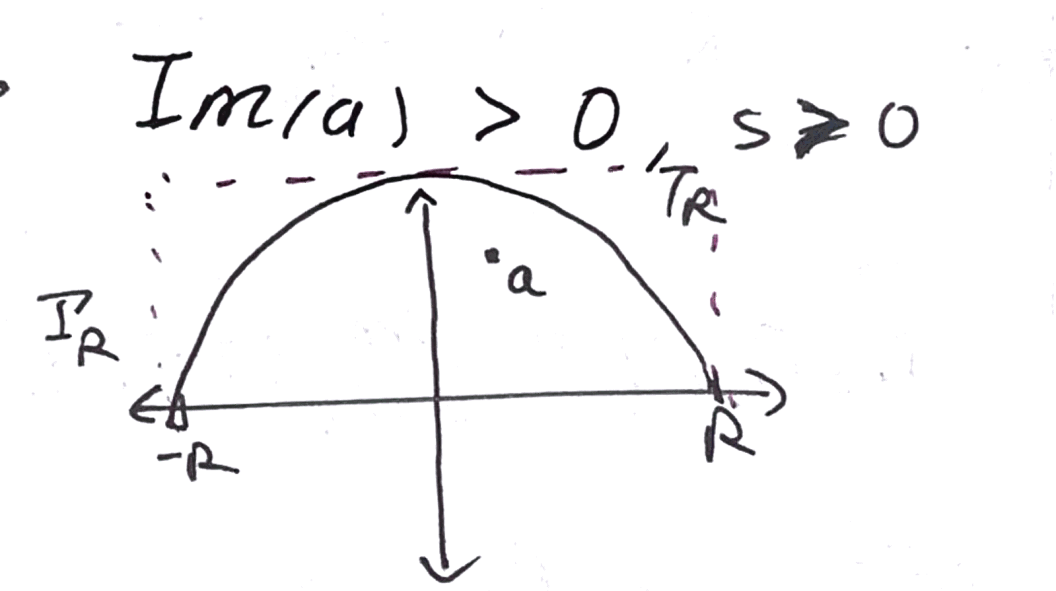
\includegraphics[width=.5\textwidth]{Figures/contour-3.png}}\]
where $R > |a|$, while we could use a rectangle, we will stick with the half-circle again. Then again Cauchys' Residue Theorem tells us that
\[\int_{\Gamma_R} f(z) dz = 2\pi i Res(f, a)\]
$a$ is a pole of order $1$ of $f$, so we have that
\[Res(f, a) = \lim_{z \to a} (z - a) \frac{e^{isz}}{z - a} = e^{isa}\]
However, we note that $f$ is actually \textbf{NOT INTEGRABLE}, so the following limit need not exist
\[\lim_{R \to \infty} \int_{-R}^R f(x) dx\]
Howebver, if $\int_{T_R} f(z) dz = 0$, then the limit would exist, and we would have
\[\lim_{R \to \infty} \int_{-R}^R f(x) dx = 2 \pi i e^{isa} = p.v \int_{-\infty}^\infty f(x) dx\]
However, we run into a problem with doing $ML$-esitmate on $\int_{T_R} f(z) dz = 0$, because it turns out it'd give us
\[|\int_{T_R} f(z) dz| \leq \frac{R}{R - |a|} \pi \]
, which does not converge to $0$ as $R \to \infty$.\\

Fortunately, we do have a workaround:
\begin{lemma}[Jordan's Lemma]
Let $C \in \Rbb$ be some fixed constant, then
\[\int_{T_R} |e^{iz}| |dz| \leq C\]
, where $|dz|$ is with respect to the Lebesgue Measure of the unit circle.
\end{lemma}

Now take $z = R e^{i \theta}$, then $dz = i R e^{i \theta} d \theta$, so we have that $|dz| = R |d \theta|$.

\begin{corollary}
If $s > 0$, then 
\[\int_{T_R} |e^{iz}| |dz| \leq C(s)\]
, where $C(s)$ is some constant dependent on $s$.
\end{corollary}

\begin{remark}
Jordan's Lemma for circles are generally hard to show, so most textbooks only prove it on a rectangle instead:
\[\fbox{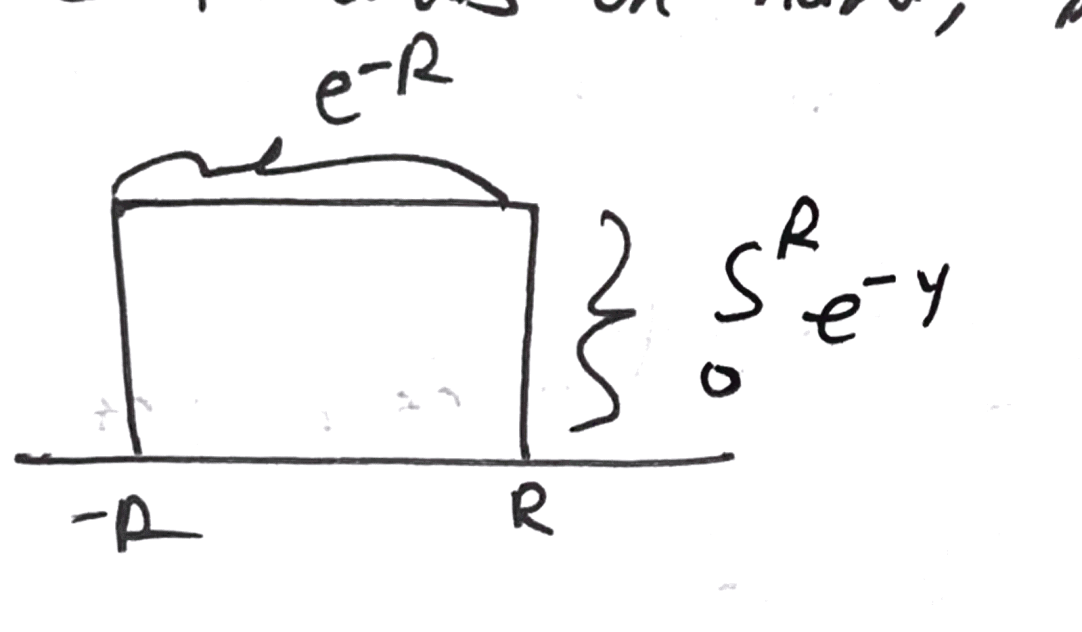
\includegraphics[width=.5\textwidth]{Figures/contour-4.png}}\]
\end{remark}

Now, using Jordan's Lemma, we have that
\begin{align*}
    |\int_{T_R} \frac{e^{isz}}{z - a} dz| &\leq \frac{1}{R - |a|} \cdot \int_{T_R} |e^{isz}| |dz|\\
    &\leq \frac{C(s)}{R - |a|}
\end{align*}
, so the limit goes to $0$ as $R \to \infty$.

\begin{question}
What about if $\Im(a) < 0$ and $s > 0$?
\end{question}

 In this case, we can either close the lower half or use a change of variables to get the same result.

\begin{question}
What about if $\Im(a) > 0$ but $s < 0$?
\end{question}

In this case, we will consider the contour
\[\fbox{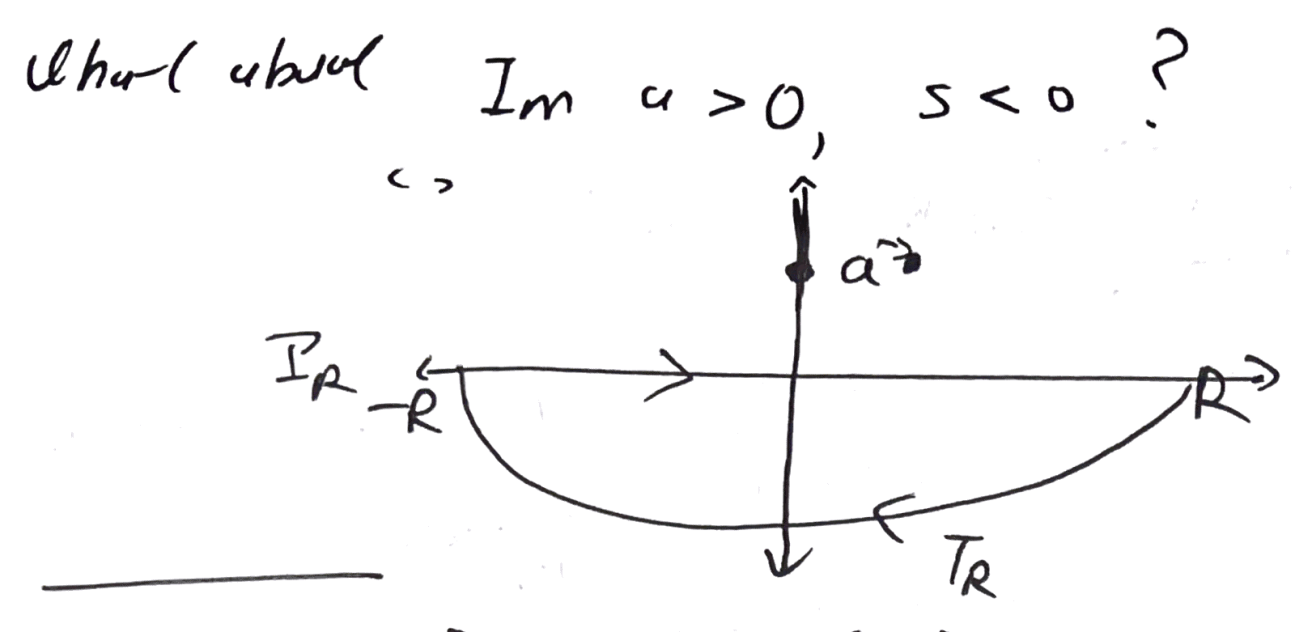
\includegraphics[width=.5\textwidth]{Figures/contour-5.png}}\]
There are no singularities inside the contour so
\[\int_{\Gamma_R} f(z) dz = 0\]
In addition, as $R \to \infty$, we also have that
\[\int_{T_R} f(z) dz = 0\]
Thus, the integral $I$ is just $0$.

\begin{question}
What if $a \in \Rbb \setminus \{0\}$ and $s > 0$?
\end{question}

In this case, consider the contour:
\[\fbox{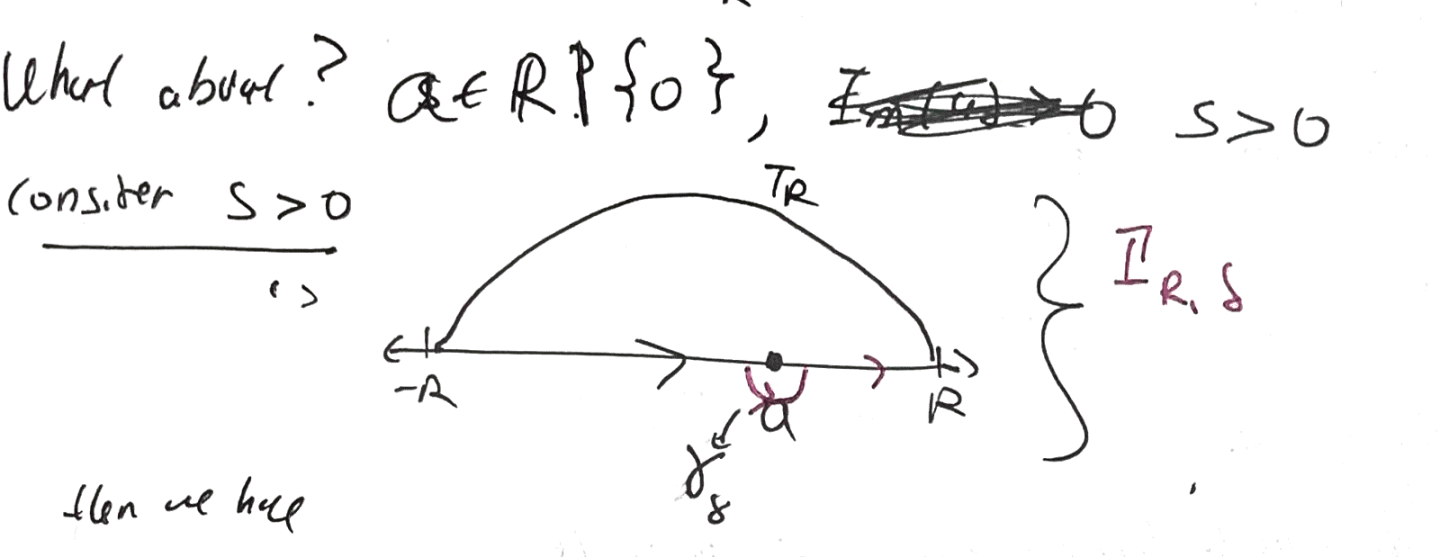
\includegraphics[width=.5\textwidth]{Figures/contour-6.png}}\]

In this, case we note that as we expand $R$ and shrink $\delta$, we have that
\[\int_{[-R, R] \setminus [a - \delta, a + \delta]} \mapsto p.v \int_{-\infty}^\infty f(z) dz\]

Cauchy's Residue Theorem tells us that
\[\int_{\Gamma_{R, \delta}} f(z) dz = 2 \pi i Res(f, a) = 2 \pi i e^{isa}\]

Jordan's Lemma tells us that
\[\lim_{R \to \infty} \int_{T_R} f(z) dz = 0 \]

Finally, taking $\delta \to 0$ gives that
\[\int_{\gamma_\delta} f(z) dz = \pi i e^{isa}\]

Thus, we have that
\[p.v \int_{-\infty}^\infty f(z) dz = 2 \pi i e^{isa} - \pi i e^{isa} = \pi i e^{isa}\]
\section{Lecture 11 - 09/30/2022}
\subsection{Computing Real Integrals with Residues - Continued}

\begin{example}
The Fresnel Integrals are the real and imaginary parts of the following integral:
\[I = \int_0^\infty e^{-ix^2} dx\]
How does one compute $I$?
\end{example}

\begin{proof}[Answer]
We will first look at the Gaussian Integral, which we are quite familiar with already:
\[\int_{0}^\infty e^{-x^2} dx = \frac{\sqrt{\pi}}{2}\]
Now for the Fresnel Integrals, consider the following contour:
\[\fbox{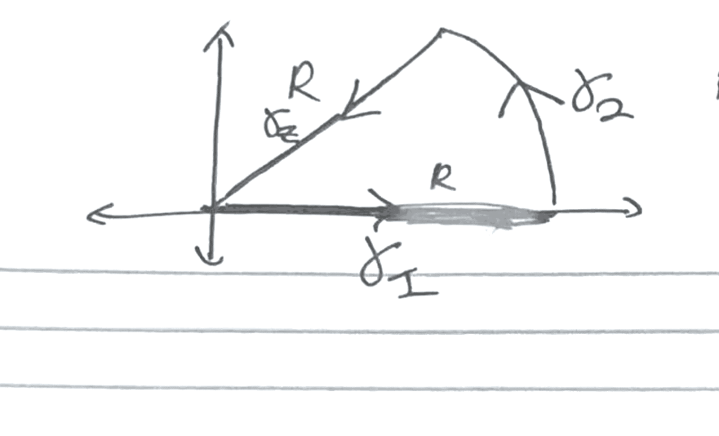
\includegraphics[width=.5\textwidth]{Figures/contour-7.png}}\]
We note that $e^{-iz^2}$ is analytic over the entire region, so Cauchy's Integral Theorem tells us that
\[0 = \int_{\gamma_1} e^{-iz^2} dz + \int_{\gamma_2} e^{-iz^2} dz + \int_{\gamma_z} e^{-iz^2} dz \]
We note that as $R \to \infty$, a similar argument as before show that the integral over $\gamma_2$ vanishes. Thus, we have that
\[I = \lim_{R \to \infty} \int_{\gamma_1} e^{-iz^2} dz = -\lim_{R \to \infty} \int_{\gamma_z} e^{-iz^2} dz\]
We can parameterize $\gamma_3$ as $z = \frac{1 + i}{\sqrt{2}} t$ from $t = R$ to $t = 0$, then
\begin{align*}
    \int_{\gamma_z} e^{-iz^2} dz &= \int_R^0 e^{-t^2} \frac{1 + i}{\sqrt{2}} dt\\
    &= -\frac{1 + i}{\sqrt{2}} \int_0^R e^{-t^2} dt\\
    \lim_{R \to \infty} \int_{\gamma_z} e^{-iz^2} dz &= -\frac{1 + i}{\sqrt{2}} \int_0^\infty e^{-t^2}\\
    &= -\frac{1 + i}{\sqrt{2}} \cdot \frac{\sqrt{\pi}}{2}
\end{align*}
\end{proof}

\subsection{Argument Principle}

Let $G$ be a bounded domain and $\partial G \in PC^1$, and consider points $p_1, ..., p_m \in G$. Suppose $f \in Hol(cl(G) \setminus \{p_1, ..., p_m\})$, meaning that $f$ is holomorphic in $\Omega \setminus \{p_1, ..., p_m\}$ where $\Omega$ is an open set containing $cl(G)$.\\

Suppose furthermore that $f(z)$ is not the constant zero function. We note that $cl(G)$ is compact, so the asusmption above implies that $f$ has finitely many zeroes in $cl(G)$. Otherwise, if $f(z)$ has infinitely many zeroes, compact sets are sequentially compact in $\Cbb$, so $f$ would containing some zero that's not isolated, violating the Uniqueness Theorem. Let $z_1, ..., z_N$ be the zeroes of $f(z)$.\\

Now assume that $f(z) \neq 0$ for all $z \in \partial G$, the Argument Principle states that:

\begin{theorem}[Argument Principle]
Let $Z$ be the number of zeros inside $G$ (counting order of the zero) and $P$ be the number of poles inside $G$ (counting order of the pole), then
\[Z - P = \frac{1}{2\pi i} \int_{\partial G} \frac{f'(z)}{f(z)} dz\]
\end{theorem}

\underline{\textbf{Note that when we say number of zeroes, we are always counting multiplicity.}}

\begin{proof}
We first note that $\frac{f'(z)}{f(z)}$ is not holomorphic on a given $z$ if and only if $z$ is one of the poles or the zeros of $f(z)$.\\\\
Since $f$ is analytic, take $a \in cl(G)$, let $f(z) = (z - a)^m g(z)$ where $g(a) \neq 0$, then we note that
\begin{align*}
    \frac{f'(z)}{f(z)} &= \frac{m(z - a)^{m-1} g(z) + (z-a)^m g'(z)}{(z - a)^m g*z(}\\
    &= \frac{m}{z - a} + \frac{g'(z)}{g(z)}
\end{align*}
Since $g(a) \neq 0$, we note that $\frac{g'(z)}{g(z)}$ is analytic in a neighborhood of $a$ and can be represented as a power series, so
\[\frac{f'(z)}{f(z)} = m(z - a)^{-1} + \sum_{n = 0}^\infty b_n (z - a)^n\]
Thus, in other words, $m$ is the coefficient of the $-1$-th power term, hence
\[res(\frac{f'(z)}{f(z)}, a) = m\]
If $a$ is one of the zeroes $z_k$, then $m$ is exactly the order of the zero.\\\\
If $a$ is one of the poles $p_k$, then $m$ is given by factoring out the Laurent Series. Clearly $m$ is exactly $-1$ times the order of the pole.\\\\
Thus, applying Residue's Theorem around the zeroes and the poles, we have that
\[Z - P = \frac{1}{2\pi i} \int_{\partial G} \frac{f'(z)}{f(z)} dz\]
\end{proof}

\begin{remark}
Why is this theorem called the \textbf{Argument Principle}? This is because $\frac{f'(z)}{f(z)}$ is actually primitive given a chosen branch, and
\[\frac{f'(z)}{f(z)} = [\log f(z)]'\]
Thus, often we sometimes rewrite the Argument Principle as
\[Z - P = \frac{1}{2\pi i} \int_{\partial G} d \log(f(z))\]
We claim that in fact
\[\frac{1}{2\pi i} \int_{\partial G} d \log(f(z)) = \frac{1}{2\pi} \int_{\partial G} d(\arg f(z))\]
\end{remark}

\begin{proof}
We first note that we can rewrite $f(z)$ in its polar coordinate form as
\[f(z) = r(z) e^{i \cdot arg(f(z))}\]
, then we have that
\begin{align*}
    \frac{1}{2\pi i} \int_{\partial G} d \log(f(z)) &= \frac{1}{2\pi i} \int_{\partial G} d(\log[r(z)e^{i \cdot arg(f(z))}])\\
    &= \frac{1}{2\pi i} \int_{\partial G} d(\log r(z)) + \frac{1}{2\pi i} \int_{\partial G} i \cdot d(arg(f(z)))\\
    &= \frac{1}{2\pi i} \int_{\partial G} d(\log r(z)) + \frac{1}{2\pi} \int_{\partial G} d(\arg f(z))
\end{align*}
It remains for us to show that $\frac{1}{2\pi i} \int_{\partial G} d(\log r(z))$ is actually $0$. We first note that by the Argument Principle, this integral is an integer. Now, since $r(z)$ is a real valued function, $\int_{\partial G} d(\log r(z))$ is real, hence the integral is also a complex number.\\\\
The only number that is both complex and integer is $0$.\\\\
Thus, we conclude that
\[\frac{1}{2\pi i} \int_{\partial G} d \log(f(z)) = \frac{1}{2\pi} \int_{\partial G} d(\arg f(z))\]
\end{proof}

\subsection{Rouche's Theorem}

Rouche's Theorem is a standard corollary of the Argument Principle. Assume the same setup as before:\\

Suppose $G$ is a bounded domain with $\partial G \in PC^1$ and $f, h \in Hol(cl(G))$:

\begin{theorem}[Rouche's Theorem]
Suppose that $|h(z)| < |f(z)|$ for all $z \in \partial G$, then the number of zeroes of $f + h$ in $G$ is the same as the number of zeroes of $f$ in $G$.
\end{theorem}

\begin{proof}
Let $\varphi(z) = \frac{f(z) + h(z)}{f(z)}$. We claim that the number of zeroes of $\varphi$ is the number of poles of $\varphi$ (inside $G$). This is because the common zeroes of $f(z) + h(z)$ and $f(z)$ would cancel out, while the rest would match, so we claim we could without choose $f, h$ such that they don't have any common zeroes.\\\\
Before we proceed with the rest of the proof, we will first justify why this is true. 
Now suppose $f(z) + h(z)$ and $f(z)$ have common zeroes $c_1, ..., c_m$ in $G$ (counting multiplicity). We note that their common zeroes have to be finite since $cl(G)$ is compact, so having a infinite number of zeroes would imply that both functions here are identically zero (by the uniqueness theorem).\\\\
Now $f(z) + h(z)$ and $f(z)$ have common zeroes $c_1, ..., c_m$ if and only if $f(z), h(z)$ have common zeroes $c_1, ..., c_m$.\\\\
Now we claim that in general, for $g \in Hol(\Omega)$ and $z_0 \in \Omega$ such that $g(z_0) = 0$, $\frac{g(z)}{z - z_0}$ has a removable singularity at $z_0$ (this just comes from the fact that its neighborhoods are bounded). So we can without loss view the quotient with the limit filled in as a holomorphic function on $\Omega$.\\\\
Applying this principle to $f(z)$ and $h(z)$, we have that
\[f(z) = \prod_{k = 1}^m (z - c_k) f_0(z), h(z) = \prod_{k = 1}^m (z - c_k) h_0(z)\]
, then the extraneous terms would cancel out but $f_0(r) \neq 0, h_0(r) \neq 0$ for any $r \in \{c_1, ..., c_m\}$.\\\\
Now, we write $\varphi(z) = 1 + \frac{h(z)}{f(z)}$, and note that
\[|\frac{h(z)}{f(z)}| < 1 \text{ on $\partial G$}\]
, so the values of $\varphi(z)$ are exactly values contained in $D_{1, 1}$ (the open disk centered at $1$ of radius $1$) by Triangle's Inequality. In particular we note this means that $Re(\varphi(z)) > 0$.\\\\
Therefore, we note that $Log \varphi(z)$ ($z \in \partial G$) is well-defined as we avoided the branch cut at $(-\infty, 0]$. Thus, it is a well-defined anti-derivative where
\[(Log \varphi(z))' = \frac{\varphi'(z)}{\varphi(z)}\]
, hence we have that
\[\int_{\partial G} \frac{\varphi'(z)}{\varphi(z)} = 0\]
Then by the argument principle, the number of zeroes and $\varphi$ is the same as the number of poles of $\varphi$ in $G$.
\end{proof}

\begin{corollary}[The Fundamental Theorem of Algebra]
Let $p(z) = \sum_{k = 0}^n a_k z^k$, where $a_n \neq 0$, then $p(z)$ has $n$ complex roots (counting multiplicity).
\end{corollary}

\begin{proof}
Take $G = D_{0, R}$ where $R > 0$ is big enough that
\[|a_n| R^n > \sum_{k = 0}^{n-1} |a_k| R^k\]
, we can find this $R$ because
\[\lim_{R \to \infty} \frac{\sum_{0}^{n-1} |a_k| R^k}{|a_n| R^n} = 0\]
We note that on $z \in \partial D_{0, R}$, $|a_n z^n| > |p(z) - a_n z^n|$, so we can take $f(z) = a_n z^n$ and $h(z) = p(z) - a_n z^n$.\\\\
Then we note that $a_n z^n$ has $n$-roots, so Rouche's Theorem tells us that $p(z)$ has $n$-roots.
\end{proof}

\subsection{Hurwitz Theorem}

\begin{definition}
Let $\{f_n\}$ be a sequence of functions, we say $f_n \to f$ converes normally in $G$ if for all compact $K \subset G$, $f_n$ converges to $f$ on $K$ uniformly.
\end{definition}

In this class, when we say $f_n$ converges to $f$ and $f_n$ are holomorphic on $G$, then we always mean that the convergence is normal!

\begin{proposition}
If $f_n$ are holomorphic functions on $G$ that converges to $f$ normally, then $f$ is also holomorphic on $G$. Furthermore, we have that $f_n^{(k)}$ converges to $f^{(k)}$ normally.
\end{proposition}

\begin{proof}
Let $R$ be a rectangle contained in $G$, since $f_n$ converges to $f$ normally, $f_n$ converges to $f$ uniformly on $R$, so we can switch the integral and limit to see that
\[0 = \lim_{n \to \infty} \int_{\partial R} f_n dz = \int_{\partial R} \lim_{n \to \infty} f(z) dz = \int_{\partial R} f(z) dz\]
, thus Morera's Theorem tells us that $f$ is holomorphic on $G$.\\\\
Now for the convergence of $f_n^{(k)}$ to $f^{(k)}$, let $K$ be a compact set in $G \subset \Omega$. For all $z \in K$, consider the disk $D_z$ small enough that $cl(D_z) \subset \Omega$, then the collection $\{D_z, z\in K\}$ form an open cover of $K$. As $K$ is compact, we can find a finite subcover $D_{z_1}, ..., D_{z_n}$.\\\\
We will without loss take $G = \bigcup_{i = 1}^n D_{z_i}$ (as we only need to show uniform convergence on $K$). This is going to be a bounded domain with piecewise smooth boundary, so we can use Cauchy's Formula for Derivatives and see that
\[f^{(k)}_n(z) - f^{(k)}(z) = \frac{k!}{2\pi i} \int_{\partial G} \frac{f_n(\xi) - f(\xi)}{(\xi - z)^{k+1}} d\xi\]
We now note that as both $K$ and $\partial G$ are compact and disjoint,
\[dist(K, \partial G) = \inf_{(x, y) \in K \times \partial G} d(x, y) = \delta > 0\]
Thus, for any $z \in K, \xi \in \partial G$, $|z - \xi| \geq \delta$, so we have that
\begin{align*}
    |f^{(k)}_n(z) - f^{(k)}(z)| \leq \frac{1}{2\pi} \frac{k!}{\delta^{k+1}} \cdot [\max ||f_n  - f||] \cdot Len(\partial G)
\end{align*}
Now since $f_n$ converges to $f$ uniformly on $G$, it converges in measure and hence $[\max ||f_n  - f||]$ shrinks to $0$ as $n \to \infty$. Thus, we have that
\[\lim_{n \to \infty} |f^{(k)}_n(z) - f^{(k)}(z)| = 0\]
, hence we have shown uniform convergence on $K$.
\end{proof}

\begin{definition}[Alternative Definition of Normal Convergence]
If for all disc $D$ such that $cl(D) \subset \Omega$, $f_n$ converges to $f$ on $D$ uniformly, then we say $f_n$ converges to $f$ normally in $\Omega$.    
\end{definition}

Note that the two definition of $f_n$ are equivalent.

\begin{theorem}[Hurwitz's Theorem]
    Suppoose $f \in Hol(\Omega)$ and $z_0 \in \Omega$ is a zero order $m$.\\\\
    Let $z_0 \in U$, where $U$ is some bounded open set, and $\partial U \in PC^1$.\\\\
    Now suppose for all $z \in cl(U) \setminus \{z_0\}$, $f(z) \neq 0$, and suppose $\{f_n\}$ converges to $f$ normally on $\Omega$, then there exists some $N \in \Nbb$ such that for all $k > N$, $f_k$ has exactly $m$ zeroes in $U$.
\end{theorem}

\begin{proof}[Proof of Hurwitz's Theorem]
    We know that $f_n$ converges uniformly to $f$ on $\partial U$ and $f_n'$ converges uniformly to $f'$ on $\partial U$. Since $f(z) \neq 0$ on $\partial U$, we note that
    \[\frac{f'_n}{f} \to \frac{f'}{f} \text{ converges uniformly on $\partial U$}\]
    Since the convergence is uniform, we also have that
    \[\frac{1}{2\pi i} \int_{\partial U} \frac{f'_n(z)}{f_n(z)} dz \to \frac{1}{2\pi i} \int_{\partial U} \frac{f'(z)}{f(z)} dz\]
    , but we note that the Argument Principle tells us that both values above are integers. Now pick some $\epsilon < \frac{1}{2}$, then there exists some $N$ such that for all $n > N$,
    \[|\frac{1}{2\pi i} \int_{\partial U} \frac{f'_n(z)}{f_n(z)} dz - \frac{1}{2\pi i} \int_{\partial U} \frac{f'(z)}{f(z)} dz| < \epsilon\]
    , and hence they are the same integer. But we note that $f'(z)/f(z)$ has no zeroes and only a pole of order $m$ while $f_n'(z)/f_n(z)$ has no poles but only zeroes.\\\\
    Thus, $f_n(z)$ has $m$ zeroes (counting multiplicity).
\end{proof}

\begin{remark}
    Note that Hurwitz's Theorem tells us that zeroes have to be appear gradually in the convergence.\\\\
    This need not be true in the real case. For example, take $f_n(x) = x^2 + \frac{1}{n}$. This is not zeroes on $\Rbb$. However, the limit is $x^2$ and has $2$ zeroes at $x = 0$. So the zeroes can just pop up out of nowhere.
\end{remark}
\section{Lecture 12}
\subsection{Remark: Normal Convergence}

Note that the following facts holds on just in $\Cbb$, but in $\Rbb^n$ in general. Recall the two definitions of normal convergence:

\begin{definition}[Equivalent Definitions of Normal Convergence]
Let $\{f_n\}$ be a sequence of functions, we say $f_n \to f$ converes normally in $G$ if:
\begin{itemize}
    \item (a) for all compact $K \subset G$, $f_n$ converges to $f$ on $K$ uniformly.
    \item or, (b) if for all disc $D$ such that $cl(D) \subset \Omega$, $f_n$ converges to $f$ on $D$ uniformly.
\end{itemize}
The two definitions are in fact equivalent.
\end{definition}

\begin{proof}
$(a) \implies (b)$ is obvious. Now, for $(b) \implies (a)$, suppose $K \subset \Omega$ is compact, then for all $z \in K$, we can choose $D_z$ be an open disk centered at $z$ small enough that $cl(D_z) \subset \Omega$.\\\\
Then the collection $\{D_z\}_{z \in K}$ form a clear open cover of $K$, so we can find a finite subcover, $D_{z_1}, ..., D_{z_n}$. $f$ converges uniformly on each $cl(D_{z_i})$, so $f$ converges uniformly on $\bigcup_{k = 1}^n D_{z_i}$, which covers $K$.
\end{proof}

How do we in general check for normal convergence? It seems like we will have to check uncountably many disks!

\begin{proposition}[Strong Covering Property]
Consider the sequence $\{K_n\}_{n = 1}^\infty \subset \Omega$ such that for all compact $K \subset \Omega$, there exists some $N$ such that $K \subset \bigcup_{n = 1}^N K_n$.\\\\
%Note that this coniditon implies that the union of the $\{K_n\}$ is
Then, $f_n$ converges to $f$ uniformly on all compact sets $K \subset \Omega$ if and only if $f_n$ converges to $f$ uniformly on each $K_n$.
\end{proposition}

\begin{proof}
The forward direction is obvious. Conversely, for any compact set $K$, find $N \in \Nbb$ such that $K \subset \bigcup_{n = 1}^N K_n$. Then the uniform convergence on each $K_n$ implies uniform convergence on all finite unions on all of $\bigcup_{n = 1}^N K_n$, hence the uniform convergence is held on $K$.
\end{proof}

\begin{remark}
In practice, for open subset $\Omega \subset \Rbb^d$, we would define each $K_n$ as
\[K_n \coloneqq \{x \in \Omega\ |\ dist(x, \Omega^c) > \frac{1}{n}, |x| \leq n\}\]
\mattie{Ask about this}
\end{remark}

\begin{definition}
We say the collection $\{K_n\}_{n = 1}^\infty$ is a \textbf{compact exhaustion} of $\Omega$ if
\[K_n \subset int(K_{n+1}) \text{ and } \bigcup_{n = 1}^\infty K_n = \Omega\]
, note that the latter implies for any compact $K \subset \Omega$, there exist $N \in \Nbb$ such that $K \subset \bigcup_{n = 1}^N K_n$
\end{definition}

\subsection{Seminorms of Holomorphic Function}

\begin{definition}
Let $Hol(\Omega)$ be the set of all holomorphic functions on $\Omega$, given $f \in \Omega$, we define the norm
\[||f||_{C(K_n)} = |\sup_{z \in K_n} f(z)|\]
When $K_n$ are points, this is called a semi-norm. $C(K_n)$ refers to the space of continuous real-valued functions on $K_n$.
\end{definition}

\begin{proposition}
If $K_n$ has the strong covering property, then $f_n$ converges to $f$ on compact sets uniformly if and only if $||f_n - f||_{C(K_n)} \to 0$ as $j \to \infty$.
\end{proposition}

\begin{remark}
An important object of study in functional analysis are what's called \textbf{Frechet Spaces}, whose topology is given by countably many semi-norms.
\end{remark}

\begin{definition}
Let $f, g \in Hol(\Omega)$, we can define a metric on $Hol(\Omega)$ as
\[p(f, g) = \sum_{n = 1}^\infty \frac{1}{2^n} \frac{||f - g||_{C(K_n)}}{1 + ||f - g||_{C(K_n)}}\]
One can verify that this is indeed a metric (more details in Conway's Book)
\end{definition}

\begin{proposition}
$f_n$ converges to $f$ uniformly on compact sets if and only if $p(f_n, f) = 0$ as $n \to \infty$.
\end{proposition}

In practice, no one would actually compute the norm or fixes a compact exhaustion. However, there are great theoretical values in this metric.

\begin{theorem}
$(Hol(\Omega), p)$ is a complete metric space.
\end{theorem}

\begin{proof}
We first note that for a compact set $K$, $C(K)$ is a complete normed space (hence a Banach Space), so we observes that
\begin{itemize}
    \item 1. $\lim_{k \to \infty} p(f_k, f) = 0$ if and only if $\lim_{k \to \infty} ||f - f_k||_{C(K_n)} \to \infty$ for all $n$.
    \item 2. $\{f_k\}$ is Cauchy with respect to $p$ on $Hol(\Omega)$ if and only if $f_k$ is Cauchy with respect to $||\cdot||_{C(K_n)}$ on $C(K_n)$ for every $n$ 
\end{itemize}
Now, every convergent sequence is Cauchy. Conversely, suppose $\{f_k\}$ is a Cauchy sequence, then since each $C(K_n)$ is a complete normed space, Hence on each $K_n$, $\{f_k\}$ converges uniformly to some limit $F_n$.\\\\
We claim that we can actually find a global function $f \in C(\Omega)$ such that $f|_{K_n} = F_n$. Indeed, we want to essentially glue each $F_n$ together, which follows from the glueing lemma that for any two continuous function $f$ on $K_1$ and $g$ on $K_2$ (within $\Cbb$ so Hausdorff) with non-empty intersection $K_1 \cap K_2$, we can extend $f$ and $g$ together into a larger continuous function.\\\\
Now, since $f$ is the limit on each $K_n$, we have that $||f_k - f||_{C(K_n)} \to 0$ as $k \to \infty$, for all $n$. Hence we have from Observation $1$ that $\lim_{k \to \infty} p(f_k, f) = 0$, so $f$ is the limit of the Cauchy seuqnece in $Hol(\Omega)$.\\\\
It remains for us to show that $f \in Hol(\Omega)$. Indeed, we note that for any $K \subset \bigcup_1^N K_j$, $f_n$ converges to $f$ uniformly, hence by Morera's Theorem, we can get that $f \in Hol(\Omega)$.
\end{proof}

\subsection{Open Mapping Theorem and Inverse Function Theorem}

Suppose $f \in Hol(z)$ (non-constant), $z_0 \in \Omega$, $f(z_0) = w_0$. Let $G$ be a bounded domain with $z_0 \in G$ and $\partial G \in PC^1$.\\\\
Furthermore, for all $z \in \partial G$, suppose we have $|f(z) - w_0| \geq \delta > 0$.\\

Does such $G$ always exist? Yes!

This is because the zeroes of the function $f(z) - w_0$ are isolated (as $f(z)$ is non-constant). Therefore, $f(z) - w_0$ has no zeroes in $cl(D_{z_0, r}) \setminus \{z_0\}$ for a sufficiently small $r$.\\

Let $w \in \Cbb$ such that $|w - w_0| < \delta$, and let $m$ be the multiplicity of the zero $z_0$ of $f(z) - w_0$

\begin{lemma}
Fix $w$ as above, the fiber $f^{-1}(w)$ has $m$ points counting multiplicity in $G$, meaning that the function $g(z) = f(z) - w$ has zeroes $z_1, ..., z_m$ (counting multiplicity)
\end{lemma}

\begin{proof}
We will apply Rouche's Theorem on this. Indeed, let $g_0(z) = f(z) - w_0$, then we note that
\[g(z) = f(z) - w = [f(z) - w_0] + [w - w_0]\]
By our setup above, we know that $|f - w_0| \geq \delta$ and $|w - w_0| < \delta$. So Rouche's Theorem tells us that both $f(z) - w_0$ and $g(z) = [f(z) - w_0] + [w - w_0]$ have the same number of zeroes, counting multiplicity.\\\\
$m$ was defined to be exactly the multiplicity of $z_0$ at $f(z) - w_0$, as we chosen $G$ small enough that $f(z) - w_0$ has no other zeroes within. 
\end{proof}

\begin{corollary}[Open Mapping Theorem]
If $f \in Hol(\Omega)$ be a non-constant function, then $f$ is an open map, meaning that for all open sets $U \subset \Omega$, $f(U)$ is open.
\end{corollary}

\begin{proof}
The argument here will run similarly to how we had above.\\\\
Let $w_0 \in f(U)$, we want to show that there exist some open set $V \subset f(U)$ that contains $w_0$.\\\\
Since $w_0 \in f(U)$, we know there exist some point $z_0 \in U$ such that $f(z_0) = w_0$. Since $U$ is open, we can find some radius $\epsilon > 0$ small enough that $cl(D_{z_0, \epsilon}) \subset U$.\\\\
Now consider the function $g(z) = f(z) - w_0$. Since $g$ is holomorphic and non-constant, the uniqueness theorem for analytic function tells us that the zeros of $g(z)$ are isolated. Hence, we can choose $\epsilon > 0$ small enough that without loss $g(z)$ only has the root $z_0$ in $cl(D_{z_0, \epsilon})$.\\\\
Since $\partial D_{z_0, \epsilon}$ is compact, and $|g(z)|$ is continuous and positive, the extreme value theorem shows that there exist some minimum value $\delta > 0$ such that $\delta$ is the minimum of $|g(z)|$ for $z$ on the boundary.\\\\
Now consider the disk $D_{w_0, \delta}$. For any $w \in D_{w_0, \delta}$, by Rouche's Theorem, write $g(z) = f(z) - w = [f(z) - w_0] + [w - w_0]$, then we note that $|g(z)| \geq \delta > |w - w_0|$, then this means that $f(z) - w_0$ and $g(z)$ have the same number of zeroes in the disk $D_{z_0, \epsilon}$.\\\\
In particular, this means that there exist some $z \in D_{z_0, \epsilon}$ such that $f(z) = w$. So in other words, $w \in f(U)$.\\\\
Hence, $D_{w_0, \delta} \subset f(U)$. In other words, $w_0 \in D_{w_0, \delta} \subset f(D_{z_0, r}) \subset U$, which implies that $f(U)$ is open.
\end{proof}

\begin{theorem}[Inverse Mapping Theorem]
Let $f \in Hol(\Omega)$, $z_0 \in \Omega$, and $f(z_0) = w_0$ but $f'(z_0) \neq 0$ (so the zero is simple). Let $G \subset \Omega$ be an open bounded set that contains $z_0$ with piecewise $C^1$ boundary.\\\\
Now suppose that, for all $z \in \partial G$, $|f(z) - w_0| \geq \delta$, then for all $w$ such that $|w - w_0|$, there exists some unique function $z$ such that $z = f^{-1}(w)$ and
\[f^{-1}(w) = \frac{1}{2\pi i} \int_{\partial G} \frac{\xi f'(\xi)}{f(\xi) - w} d\xi\]
\end{theorem}
\section{Lecture 13 - 10/05/2022}

\subsection{Inverse Mapping Theorem - Continued}

Recall that per the setting of the Inverse Mapping Theorem:
\begin{itemize}
    \item Let $f \in Hol(\Omega)$ and $z_0 \in \Omega$, $f(z_0) = w_0$ and $f'(z_0) \neq 0$
    \item $G$ is a bounded domain such that $cl(G) \subset \Omega$ (in textbook we choose $D_{z_0, p}$) and $\partial G \in PC^1$
    \item $|f(\xi) - w_0| \geq \delta$ for all $\xi \in \partial G$
    \item $f(z) \neq w_0 \forall z \in G$ (possible because all zeroes of non-constant analytic functions are isolated)
\end{itemize}

\begin{theorem}[Inverse Function Theorem]
Given the setup above, then for all $w$ such that $|w - w_0| < \delta$, there exists a unique $z$ in $G$ such that $f(z) = w$ and
\[f^{-1}(w) = z = \frac{1}{2\pi i} \int_{\partial G} \frac{\xi f'(\xi)}{f(\xi) - w} d\xi\]
\end{theorem}

\begin{proof}
\textbf{Existence and uniquenss are given by Rouche's Theorem.} Indeed, by the Argument Principle, we note that
\[\# \text{ of zeroes of $f(z) - w$ in $G$ } = \frac{1}{2\pi i} \int_{\partial G} \frac{f'(\xi)}{f(\xi) - w} d\xi\]
We note that we can rewrite
\[f(z) - w = [f(z) - w_0] + [w_0 - w]\]
\[|f(z) - w_0| \geq \delta, |w_0 - w| < \delta, \text{ on $\partial G$}\]
So Rouche's Theorem tells us that $f(z) - w$ and $f(z) - w_0$ has the same number of zeroes. But we note that we chose $f(z) - w_0$ to only have one zero, and it's a zero of order $1$ by condition given, so in other words $f(z) - w$ has exactly $1$ solution, hence uniqueness and existence are both proven.\\\\
\textbf{For the formula given, } we first note that the formula
\[\frac{\xi f'(\xi)}{f(\xi) - w}\]
has a unique singularity at $\xi = f^{-1}(w)$, which is a pole of order $1$ by construction. We can calculate its residue as
\begin{align*}
    Res(\frac{\xi f'(\xi)}{f(\xi) - w}, \xi = z) &= \lim_{\xi \to z} \frac{\xi f'(\xi)}{f(\xi) - w} \cdot (\xi - z)\\
    &= z f'(z) \lim_{\xi \to z} \frac{\xi - z}{f(\xi) - w}\\
    &= z f'(z) \lim_{\xi \to z} \frac{\xi - z}{f(\xi) - f(z)} \tag*{$w$ is defined to be $w = f(z)$}\\
    &= z f'(z) \frac{1}{f'(z)}\\
    &= z
\end{align*}
Then apply Cauchy's Residue Theorem gives us
\begin{align*}
    \frac{1}{2\pi i} \int_{\partial G} \frac{\xi f'(\xi)}{f(\xi) - w} d\xi &= \frac{2\pi i}{2\pi i} Res(\frac{\xi f'(\xi)}{f(\xi) - w}, \xi = z)\\
    &= Res(\frac{\xi f'(\xi)}{f(\xi) - w}, \xi = z)\\
    &= z\\
    &= f^{-1}(w)
\end{align*}
\end{proof}

Note that the local solvability of $f$ is just a standard result that can follow from Real Analysis too. However, the formula is more significant.

\subsection{Winding Numbers}

Let $\gamma: [a, b] \to \Cbb$ be a continuous function such that $\gamma(a) = \gamma(b)$ (This is a $C^0$-closed-path). We will denote $\Gamma$ as the image of $\gamma$ in $\Cbb$.\\

Without loss of generality, we can view $\gamma$ as a function:
\[\gamma: \Tbb \to \Cbb\]
, where $\Tbb \coloneqq \frac{\Rbb}{\Zbb}$ is the $1$-dimensional torus given by an equivalence relation on $\Rbb$, where we say $a \sim b$ if $a - b \in \Zbb$.

\begin{definition}
Let $\gamma$ be as before and let $z \in \Cbb \setminus \Gamma$, then we define the \textbf{winding number} as
\[w(\gamma, z) \coloneqq \frac{1}{2\pi i} \int_{\Gamma} \frac{1}{\xi - z} d\xi\]
\end{definition}

\begin{proposition}
$w(\gamma, z)$ is an integer valued function.
\end{proposition}

\begin{proof}
The proof is similar to the idea behind the Argument Principle, but we do not assume $\gamma$ is $C^1$. We first use the Lebesgue Number Lemma to split $\Gamma$ into small enough intervals such that $\frac{1}{\xi - z}$ locally has anti-derivatives on each interval (up to the choice of some branch):
\[log(\xi - z) + 2\pi i k, k \in \Zbb\]
As we move from one interval to another, we want to continue the branch we are previously on. We don't know what the branch is exactly, but this would form a telescoping series of primitivies, and the entire integral will evaluate to
\begin{align*}
    \frac{1}{2\pi i} \int_{\Gamma} \frac{1}{\xi - z} d\xi &= \frac{1}{2\pi i} [log(\xi - z) + 2\pi i k_1 - log(\xi - z) - 2\pi i k_2]\\
    &= \frac{2\pi i}{2\pi i}(k_1 - k_2)\\
    &= k_1 - k_2 \in \Zbb
\end{align*}
\end{proof}

\begin{proposition}
$w(\gamma, z)$ measures the number of times (sign given by whether it's counter-clockwise or clockwise) $\gamma$ wraps around $z$.
\end{proposition}

\begin{proof}[Proof Idea]
We note that $\gamma$ is homotopy equivalent to a circle, so the value of the integral doesn't change if we switch $\gamma$ to a circle of some positive radius around $z$. The branch choice given in the previous proposition actually follows in a circle (when viewed as a Riemann Surface), so the loop on the circle does measure the numbers of times it wraps around $z$. This is an invariant around homotopy equivalence.
\end{proof}

\begin{definition}
We say that $\gamma$ is a \textbf{generalized path} if $\gamma: \Tbb_1 \sqcup \Tbb_2 ... \sqcup \Tbb_n \to \Cbb$ and $\gamma$ restricted to each $\Tbb_k$ is a $C^0$-closed-path. In other words, $\gamma$ is intuitively the disjoint union of finitely many closed paths.
\end{definition}

\begin{remark}
Let $\gamma$ be a generalized path, and consider the function $z \mapsto W(\gamma, z)$. This is a well-defined function on $\Cbb \setminus Im(\gamma)$ and is moreover analytic on the same domain (this follows from Morera's Theorem). Thus, analyticity implies continuity, and for $W(\gamma, z)$ to be a continuous integer value, this means that $W(\gamma, z)$ is constant on each connected component of $\Cbb \setminus Im(\gamma)$. We sometimes call this the \textbf{index} of $\gamma$ at $z$.
\end{remark}

\subsection{Generalized Residue Theorem}

\begin{theorem}[Generalized Residue Theorem]
Let $\gamma$ be a generalized path in $\Omega$, and say $f \in Hol(\Omega \setminus \{z_1, ..., z_n\})$, and suppose for all $k$, $z_k \not \in Im(\gamma)$. Then
\[\int_{\gamma} f(z) dz = 2 \pi i \sum_{k = 1}^n w(\gamma, z_k) \cdot Res(f, z_k)\]
\end{theorem}

Before, we prove this theorem, we will introduce another theorem.

\begin{theorem}\label{thm::zero_path_thm}
Let $\gamma$ be a generalized path in $\Omega$, such that
\[W(\gamma, z) = 0, \text{ for all } z \not \in \Omega\]
(Note that this is true for any simply connected domain $\Omega$. If $\Omega$ has holes, then this is say that $\gamma$ avoids these holes). Then we have that
\[\int_\gamma f(z) dz = 0, \text{ for all $f \in Hol(\Omega)$}\]
\end{theorem}

\begin{proof}
Textbook (to be added)
\end{proof}

It turns out that Theorem~\ref{thm::zero_path_thm} actually implied the Generalized Residue Theorem.

\begin{proof}[Proof of the Generalized Residue Theorem]
Consider contours $\gamma_1, ..., \gamma_n$ be circles of small enough radius, each wrapping around $z_1, ..., z_n$ counterclock direction:
\[\fbox{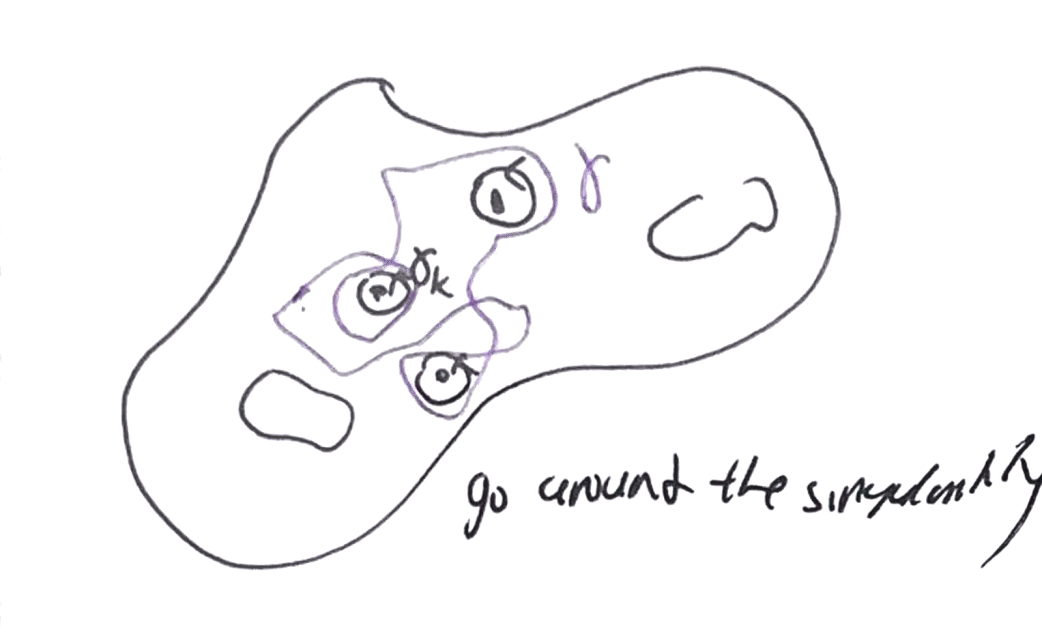
\includegraphics[width=.5\textwidth]{Figures/gen_path.png}}\]
Then consider the path $\hat{\gamma}$ given by
\[\hat{\gamma} \coloneqq \gamma - \bigcup_{k = 1}^n W(\gamma, z_k) \gamma_k\]
Then we note that for all $z \not in \Omega$, $W(\hat{\gamma}, z) = 0$ because the index of $\hat{gamma}$ at these points is reduced to $0$.\\\\
So Theorem~\ref{thm::zero_path_thm} tells us that
\begin{align*}
    0 &= \int_{\hat{\gamma}} f(z) dz\\
    &= \int_{\gamma} f(z) dz - \sum_{k = 1}^n \int_{\gamma_k} W(\gamma, z_k) f(z) dz\\
    &= \int_{\gamma} f(z) dz - [2 \pi i \sum_{k = 1}^n w(\gamma, z_k) \cdot Res(f, z_k)]
\end{align*}
\end{proof}
\section{Lecture 14 - 10/07/2022}

\subsection{Generalized Cauchy's Theorem}

Last class, recall we discussed the Generalized Residue Theorem, whose proof relied on Theorem~\ref{thm::zero_path_thm}. 
 Theorem~\ref{thm::zero_path_thm} above is sometimes called the \textbf{Generalized Cauchy's Theorem}, not to be confused with the \textbf{Generalized Residue Theorem} that we proved last lecture.

\begin{theorem}
    Let $\gamma$ be a generalized closed path (ie. it is a union of finitely many closed paths) in $\Omega$, such that for all $z \notin \Omega$,
    \[w(\gamma, z) = 0\]
    Then, we have that for all $f \in Hol(\Omega)$,
    \[\int_\gamma f(z) dz = 0\]
\end{theorem}

Before proving this, we will first state a lemma:

\begin{lemma}
    Let $K$ be a compact subset of open $\Omega$ (ie. $K \subset \Omega$), then there exists some bounded open set $G$ with $\partial G \in PC^1$ such that:
    \begin{itemize}
        \item $cl(G) \subset \Omega$
        \item $dist(K, G^c) \geq \delta > 0$
    \end{itemize}
\end{lemma}

\begin{proof}
    Since $K$ is compact and $\Omega^c$ is closed, we know that $dist(K, \Omega^c)$ must be positive (or else they would intersect). So let's pick some $\delta$ such that $dist(K, \Omega^c) \geq 4 \delta > 0$.\\\\
    Now consider a $\delta$-grid of $\Omega$ (split $\Omega$ into squares of side length $\delta$), and consider
    \[G \coloneqq int(\bigcup_{\text{$Q$ is a square on the $\delta$-grid,}\ dist(K, Q) \leq \delta} Q)\]
    Note, that we might create a $G$ where it does have a self-intersection on the boundary, which would not make it $PC^1$, in this case, we would add a little square on the corner to ``nudge" the boundary away:
    \[\fbox{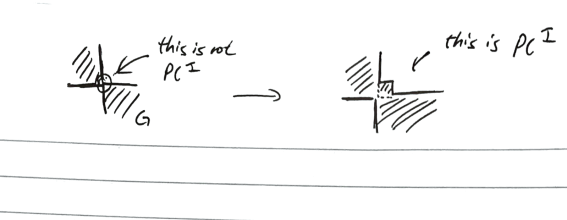
\includegraphics[width=.5\textwidth]{Figures/pc1.png}}\]
    Then we can check that
    \[dist(K, G^c) = dist(K, \partial G) \geq \delta\]
    If this is not true, then our $G$ would have to be surrounded by other cubes whose distance to $Q$ is less than $\delta$, and hence we are not looking at the boundary of $G$.
\end{proof}


\begin{proof}[Proof of Theorem~\ref{thm::zero_path_thm}]
    Recall that $f \in Hol(f)$, and consider
    \begin{align*}
        \int_\gamma f(z) dz &= \int_\gamma \frac{1}{2\pi i} \int_{\partial G} \frac{f(\xi)}{\xi - z} d\xi dz \tag*{Since f is holomorphic, use Cauchy's Integral Formula}\\
        &= \int_{\partial G} \frac{-f(\xi)}{2\pi i} \int_\gamma \frac{1}{z - \xi} dz d\xi \tag*{Fubini's Theorem}
    \end{align*}
    Now for any $\xi \in \Omega^c$, we claim that
    \[\int_\gamma \frac{1}{z - \xi} dz = 0\]
    Since $G \subset \Omega$, we have that $\Omega^c \subset G^c$. Thus, any connected component of $\Omega^c$ is contained in some connected component of $G^c$.\\\\
    If a bounded connected component $C$ of $G^c$ does not intersect with $\Omega^c$, we just add it to $G$ (take $G'$ = $G \cup C$ to be the new $G$). So we can without loss assume that any bounded component of $G^c$ intersect with $\Omega^c$.\\\\
    Thus, for all $\xi$ in such bounded component of $G^c$, 
    \[\int \frac{1}{z - \xi} dz = 0\]
    Indeed, consider the diagram:
    \[\fbox{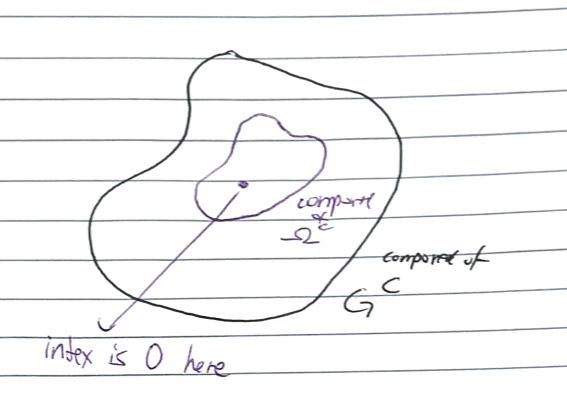
\includegraphics[width=.5\textwidth]{Figures/bounded_zero.png}}\]
    Recall that by assumption, the index of any point in $\Omega^c$ is $0$. Since the winding number is an analytic (thus continuous) function, this means that the index of every point on this one bounded component of $G^c$ is identically zero.\\\\
    Now, on unbounded connected components of $G^c$, we can't just add this to $G$ since we still want $G$ to be bounded. But we note that $W(\gamma, \xi) = 0$. This is because as $|\xi| \to \infty$, we can eventually find some $\xi$ such that the loop $\gamma$ does not enclose it. The fact that the entire component has index $0$ follows from the fact that the winding number is a continuous function. \\\\
    Thus, we have that
    \[\int_\gamma f(z) dz = \int_{\partial G} \frac{-f(\xi)}{2\pi i}  \cdot 0 d\xi  = 0\]
\end{proof}

\begin{remark}
    On the complex plane $\Cbb$, we can add a point at infinity as the one-point compactification of $\Cbb$, which we denote as $\hat{\Cbb}$. This is called the \textbf{Riemann Sphere}.\\\\
    Then on $\hat{\Cbb}$, $\Omega$ is a simply connected domains if and only if $\hat{\Cbb} \setminus \Omega$ is connected. The proof in the book is rather tedious and uses many details, but there's a standard topological proof of this using the Riemann Mapping Theorem, which we will discuss later.
\end{remark}

\begin{corollary}
    Let $\Omega \subsetneq \Cbb$ be a bounded domain and $\Cbb \setminus \Omega$ is connected, then for any $z_0 \in \Cbb \setminus \Omega$, there exists a branch of $\log(z - z_0)$ in $\Omega$.
\end{corollary}

\begin{proof}
    Fix some $w_0 \in \Omega$ and take $a_0$ as one of the values of $\log (w_0 - z_0)$ (this is defined up to $2\pi i$, but we just choose one). Now we define the branch $\log z - z_0$ as
    \[\log(z - z_0) = a_0 + \int_{w_0}^z \frac{d\xi}{\xi - z_0} \]
    Note that our integral does not depend on the choice of pathes, as shown by the Generalized Cauchy's Theorem, so our branch is well-defined.
\end{proof}

\subsection{Jump Theorem for Cauchy Integrals}

Let $\gamma$ be a $C^1$-curve and suppose $f$ be a $C^1$ compact-supported function on $\gamma$ (denote this as $f \in C^1_c(\gamma)$, note this need not be analytic). We want $f$ to be compactly supported to avoid any convergence issue.

There's a slight abuse of notation going on here, by $f \in C^1(\gamma)$, we actually mean that for $\gamma: [a, b] \to \Cbb$, $f \circ \gamma$ is $C^1$.

Define the function
\[F(z) \coloneqq \frac{1}{2\pi i} \int_\gamma \frac{f(\xi)}{\xi - z} d\xi\]

We note that $F \in Hol(\gamma^c)$, now take some point $z_0 \in \gamma$, and consider
\[F_{\pm}(z_0) \coloneqq \lim_{z \to z_0} F(z)\]
, where ``$+$" is from inside and ``$-$" is from outside.\\\\

Naively, we claim we could just exchange the limit and the integral, then
\[F_{\pm}(z_0) = \frac{1}{2\pi i} \int_{\gamma} \frac{f(\xi)}{\xi - z_0} d\xi\]

However, in general the integral is not integrable around $z_0$, so we next hope that we could converge it to some principal value:
\[F_{\pm}(z_0) = \frac{1}{2\pi i} p.v. \int_{\gamma} \frac{f(\xi)}{\xi - z_0} d\xi\]
, where we say that
\[p.v. \int_\gamma ... = \lim_{\delta \to 0} \int_{\gamma \setminus D_{z_0, \gamma}} ...\]

This, however, is also problematic! Indeed, consider the following counter-example where $\gamma$ is a circle and $f(z) = 1$ is the constant $1$ function:
    \[\fbox{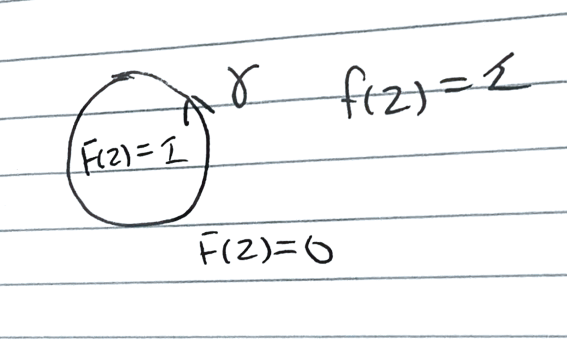
\includegraphics[width=.5\textwidth]{Figures/cauchy_jump.png}}\]
, but $F(z)$ is the winding number and is hence $1$ inside and $0$ outside. So the limit does not even converge.

The next best thing we get, is fortunately true. This is sometimes also called the \textbf{Jump Theorem}:

\begin{theorem}[Plemelji-Sokhotsky formula]
    \[F_{\pm}(z_0) = \frac{1}{2\pi i} p.v. \int_\gamma \frac{f(\xi)}{\xi - z_0} d\xi \pm \frac{1}{2} f(z_0)\]
\end{theorem}

\begin{remark}
    Note that the theorem is actually also true for just curves (need not be closed). In this case, by inside and outside we mean the orientation given by the \textbf{left leg rule}.
\end{remark}

Before we prove the theorem, we first make an observation:
\begin{observation}\mattie{Why??}
    We note that the theorem is actually a local theorem. If $f \in C^1(\gamma)$ and $f \equiv 0$ in a small neighborhood of $z_0$, then everything is trivial as
    \[F_{\pm}(z_0) = \frac{1}{2\pi i} \int \frac{f(\xi)}{\xi - z_0} d\xi\]
    Therefore, we can without loss just assume $f \in C^1(D_{z_0, \delta_0})$.
\end{observation}

\begin{proof}[Proof of Jump Theorem]
    \begin{align*}
        \int_\gamma \frac{f(\xi)}{\xi - z_0} d\xi &= \int_\gamma \frac{f(\xi) - f(z)}{\xi - z} d\xi + \int_\gamma \frac{f(z)}{\xi - z} d\xi
    \end{align*}
    Note that as we take $z \to z_0$ on the left integral, we can apply the Dominated Convergence Theorem as $|\nabla f| \leq M$ in $D_{z_0, \delta_0}$ is bounded on compact set, and everything is compactly supported
    \begin{align*}
        \lim_{z \to z_0}  \int_\gamma \frac{f(\xi) - f(z)}{\xi - z} d\xi &= \int_\gamma \lim_{z \to z_0} \frac{f(\xi) - f(z)}{\xi - z} d\xi \tag*{Dominated Convergence Theorem}\\
        &= \int_\gamma \frac{f(\xi) - f(z_0)}{\xi - z_0} d\xi\\
        &= p.v. \int \frac{f(\xi)}{\xi - z_0} d\xi - p.v. \int_\gamma \frac{f(z_0)}{\xi - z_0} d\xi \tag*{Existence of Principal Values left as Exercise}
    \end{align*}
    For the right integral, we will evaluate
    \begin{align*}
        \lim_{z \to z_0} \int_\gamma \frac{f(z)}{\xi - z} d\xi
    \end{align*}
    We will finish the proof in the next lecture.
\end{proof}
\section{Lecture 15 - 10/12/2022}

\subsection{Jump Theorem for Cauchy Integrals}
Let $\gamma \in PC^1$ with image $\Gamma := \gamma([a, b]) \subset \Cbb$, and let $f(z)$ be a continuous function on $\Gamma$.

\begin{definition}
The \textbf{Cauchy Integral} of $f(z)$ along $\gamma$ is the function
\[F(\xi) \coloneqq \frac{1}{2\pi i} \int_\gamma \frac{f(z)}{z - \xi} dz, \forall \xi \in \Cbb \setminus \Gamma\]
Note that as we take $\xi$ to infinity, $F(\xi) = 0$. Furthermore, $F(\xi)$ is analytic on $\Cbb \setminus \Gamma$ since it could be represented in power series by geometric expansion.
\end{definition}

\begin{example}
If $\gamma$ is a closed loop and $f(z)$ is identically $1$, then the Cauchy integral of $f(z)$ around $\gamma$ is exactly the winding number $F(\xi) = w(\gamma, \xi)$ of $\gamma$ around $\xi$, which is either $1$ if the point is inside or $0$ if the point is outside.
\end{example}

\begin{theorem}[Plemelj-Sokhotsky Theorem]
Let $\gamma$ be a simple $C^1$-closed curve, and $f \in C^1_\Cbb(\gamma)$. Note that the Cauchy Integral $F(z) = \frac{1}{2\pi i} \int_\gamma \frac{f(\xi)}{\xi - z} d\xi$ is undefined for any $z \in \gamma$ but is defined on the interior and exterior of the curve, which we will denote by $F_+$ for interior and $F_-$ for exterior respectively.\\\\
Now take $z_0$, we have that
\[F_{\pm}(z_0) = \frac{1}{2\pi i} p.v. \int_\gamma \frac{f(\xi)}{\xi - z_0} d\xi \pm \frac{1}{2} f(z_0)\]
\end{theorem}

\begin{proof}
    First we rewrite
    \[\int_\gamma \frac{f(\xi)}{\xi - z} d\xi = \int_\gamma \frac{f(\xi) - f(z)}{\xi - z} d\xi + \int_\gamma \frac{f(z)}{\xi - z} d\xi\ (*)\]
    Now let $\delta > 0$ be chosen appropriately and consider the disk $D_{z_0, \delta}$ such that the domain of where $f$ is homolomorphic contains the closure of the disk (recall $f$ being holomorphic on compact $\gamma$ means there exists some open set containing $\gamma$ that $f$ is holomorphic on). Then since $\nabla f$ is a continuous function on compact $\overline{D_{z_0, \delta}}$, $|\nabla f|$ is bounded on the the disk.\\\\
    Thus, by Dominated Convergence Theorem, as we take the limit as $z \to z_0$:
    \[\lim_{z \to z_0} \int_\gamma \frac{f(\xi) - f(z)}{\xi - z} d\xi = \int_\gamma \lim_{z \to z_0} \frac{f(\xi) - f(z)}{\xi - z} d\xi = p.v. \int_\gamma \frac{f(\xi)}{\xi - z_0} d\xi - p.v. \int_\gamma \frac{f(z_0)}{\xi - z_0} d\xi\]
    There are two more things that we want to check:
    \begin{itemize}
        \item The principal value of $\int_\gamma \frac{1}{\xi - z_0} d\xi$ exists
        \item The following limit is true \[\lim_{z \to z_0, \text{interior}} \int_\gamma \frac{1}{\xi - z} d\xi = p.v. \int_\gamma \frac{d\xi}{\xi - z_0} + \pi i\]
    \end{itemize}
    Then it follows from the limit and our prior computation that:
    \begin{align*}
        F_+(z_0) &= \frac{1}{2\pi i} \cdot [p.v. \int_\gamma \frac{f(\xi)}{\xi - z_0} d\xi  - p.v. \int_\gamma \frac{f(z_0)}{\xi - z_0} d\xi] + \frac{1}{2\pi i} \cdot [p.v. \int_\gamma \frac{f(z_0) d\xi}{\xi - z_0} + f(z_0) \pi i]\\
        &= \frac{1}{2\pi i} p.v. \int_\gamma \frac{f(\xi)}{\xi - z_0} d\xi + \frac{1}{2} f(z_0) \tag*{We can cancel the principal values because they exist}
    \end{align*}
    A similar argument will also prove the case for $F_{-}(z_0)$. It then remains for us to prove the two claims:
    \begin{enumerate}
        \item For existence, let $\gamma_\delta \coloneqq \gamma \cap D_{z_0, \delta}$ and let $\gamma^\delta \coloneqq \gamma \setminus \gamma_\delta$. In other words, the latter is $\gamma$ with its path in the disk removed, then we have that
        \[\int_\gamma \frac{d\xi}{\xi - z} = \int_{\gamma_\delta} \frac{d\xi}{\xi - z} + \int_{\gamma^\delta} \frac{d\xi}{\xi - z}\]
        Now consider the following contour:
        \[\fbox{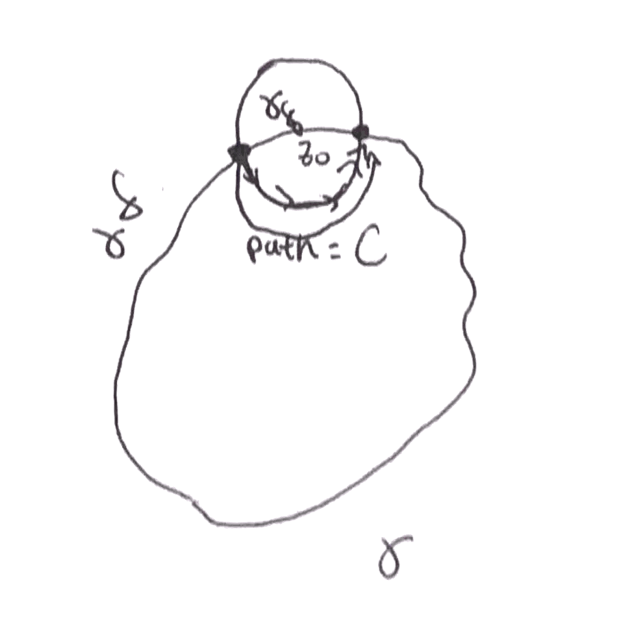
\includegraphics[width=.4\textwidth]{Figures/gamma-delta.png}}\]
        Then by Cauchy's Theorem
        \[\int_{\gamma_\delta} - \int_C = 0\]
        Hence we have that
        \[\int_\gamma \frac{d\xi}{\xi - z} = \int_{C} \frac{d\xi}{\xi - z} + \int_{\gamma^\delta} \frac{d\xi}{\xi - z} \]
        Then as we take the limit and exchange it with the integral using uniform convergence:
        \[\lim_{z \to z_0, \text{inside}} \int_\gamma \frac{d\xi}{\xi - z} = \int_{C} \frac{d\xi}{\xi - z_0} + \int_{\gamma^\delta} \frac{d\xi}{\xi - z_0}\]
        So the principal value exist (because the limit exist as the new contour we made it avoid $z_0$) and the value of the integral does not depend on $\delta$.
        \item Note that $\lim_{z \to z_0, \text{interior}} \int_C \frac{1}{\xi - z} d\xi = i \cdot \theta_\gamma$, where $\theta_\gamma$ is the angle of the arc made with $C$. Then as $\delta \to 0$, $\theta_\delta \to \pi$ as $\gamma$ is continuous. 
        \item So we have that $\lim_{\delta \to 0} \int_C \frac{d\xi}{\xi - z_0} = \pi i$
        \item We note that as $z \to z_0$, $\delta \to 0$, so
        \[\lim_{z \to z_0} \int_\gamma \frac{d\xi}{\xi - z} = \lim_{z \to z_0} \int_{C} \frac{d\xi}{\xi - z_0} + \int_{\gamma^\delta} \frac{d\xi}{\xi - z_0} = \pi i + p.v. \int_\gamma \frac{d\xi}{\xi - z_0}\]
    \end{enumerate}
\end{proof}

\subsection{Conformal Mappings}

In Real Analysis, we have often discussed the angle between two arbitrary vectors:
\begin{definition}
    Consider two non-zero vectors $\Vec{u}, \Vec{v} \in \Rbb^n$, the \textbf{angle} between $\Vec{u}$ and $\Vec{v}$ is
    \[\cos(\alpha) \coloneqq \frac{\Vec{u} \cdot \Vec{v}}{||\Vec{u}|| ||\Vec{v}|| },\ 0 \leq \alpha \leq \pi\]
\end{definition}

In complex analysis, we can also define it in a similar way:
\begin{definition}
    Let $z, w \in \Cbb$ be two non-zero complex numbers, then
    \[\text{angle}(z, w) \coloneqq \text{arg}(z \overline{w})\]
\end{definition}

\begin{definition}[Conformal Map]
    Let $\Omega \subseteq \Rbb^n$ be open, we say a map $f: \Omega \to \Rbb^n$ is conformal at $x_0 \in \Omega$ if $f$ preserves angles between tangent lines of directed curves through $x_0$ (not necessarily length). 
\end{definition}

\begin{fact}
    If $f$ is conformal at $x_0$ then the Jacobian of $f$ at $x_0$ is an orthogonal matrix multiplied by some scalars.
\end{fact}

In $\Rbb^n$, $n > 2$, there's usually not a lot of choices for conformal maps - you only really have translations, rotation, flip, and occasionally ``blow ups".\\

In $\Cbb$ ($n = 2$), it turns out that the conformal mappings $f$ are either orientation preserving or orientation reversing:
\begin{itemize}
    \item If $f$ is analytic whose $f'(z_0) \neq 0$, then $f$ is conformal and preserves orietnation
    \item If $f$ is anti-analytic (ie. $z \mapsto f(\overline{z})$ is analytic, or $f(z) = \sum a_k \overline{(z - z_0)}^k$) with non-zero derivative, then this preserves angles but reverses the orientation.
\end{itemize}

\begin{definition}
    Let $f \in \text{Hol}(\Omega)$ and $f: \Omega \to G \subseteq \Cbb$. We say that $f$ is a \textbf{conformal map} from $\Omega$ to $G$ if $f$ is bijective in $\Omega$.
\end{definition}

\begin{proposition}
    If $f \in \text{Hol}(\Omega)$ is injective, then $f'(z) \neq 0$ for all $z \in \Omega$.
\end{proposition}

\begin{proof}
    Suppose there exist some $z_0 \in \Omega$ such that $f'(z_0) = 0$, then let's also denote $f(z_0) = w_0$. We could write out the Taylor expansion of $f$ at $z = z_0$ as
    \[f(z) = f(z_0) \cdot (z - z_0)^0 + \sum_{q = 1}^\infty a_q (z - z_0)^q = w_0 + \sum_{q = 1}^\infty a_q (z - z_0)^q = w_0 + (z - z_0)^k \cdot f_0(z)\]
    where $f_0$ is obtained by factoring out $(z - z_0)$ as much as one could so that $f_0(z_0) \neq 0$. Note that since $f'(z_0) = 0$, $z_0$ is a zero of order $2$, so we have that $k \geq 2$.\\\\
    Then for $w \neq w_0$ such that $w_0 - w$ sufficiently small, we can write $f(z) - w = (f(z) - w_0) + (w_0 - w)$ such that $|f(z) - w_0| > |w_0 - w|$ on a circle centered at $z_0$.\\\\
    Then we note that the number of zeroes $f(z) - w_0$ has exactly $k \geq 2$ inside the circle, so by Rouche's Theorem, $f(z) - w_0 + w_0 - w = f(z) - w$ has exactly two zeroes inside the circle.\\\\
    There're two cases, either $f(z)$ has a zero of multiplicity at least $2$ other than $w_0$, or $f(z)$ has at least two distinct points that get mapped to $w$, which contradicts injectivity.\\\\
    Hence $f(z) - w$ has a zero of multiplicity two, but we can restrict our circle around $z_0$ such that $f'(z) \neq 0$ for all $z \neq z_0$ (since roots are isolated for non-constant analytic functions, and $f$ clearly is not constant). Hence $(f(z) - w)' = f'(z)$ cannot be zero around here, so its zero has multiplicity less than 2, contradiction.
\end{proof}

There's a very important theorem about conformal mapping that we will spend many lectures to build up to prove - the Riemann Mapping Theorem:

\begin{theorem}
    Let $U \subseteq \Cbb$ be a non-empty, simply-connected domain that is not the entire $\Cbb$, then there exists a conformal map $f$ from $U$ to the unit disk $\mathbb{D}$. Furthermore, if we fix $z_0 \in U$ and require $f(z_0) = 0$ and $f'(z_0) > 0$ (derivative is real valued), then $f$ is unqiue.
\end{theorem}

\begin{remark}
    There's no analog of the Riemann Mapping Theorem for $n > 2$ in $\Rbb^n$,
\end{remark}

\begin{definition}
    Let $f: \Omega \to \Cbb$, we say $f$ is univalent if $f$ is holomorphic and injective on $\Omega$. In particular, the univalent function $f$ on $\Omega$ is a conformal map of $\Omega$ to $f(\Omega)$.
\end{definition}

\begin{definition}[Riemann Sphere]
    We define the \textbf{Riemann Sphere} (or the ``extended complex plane") as $\hat{\Cbb} \coloneqq \Cbb \cup \{\infty\}$ as the one point compactification of $\Cbb$. Recall $\Cbb$ is topologically equivalent to $\Rbb^2$, then this process turns $\hat{\Cbb}$ topologically equivalent to $S^2$.
\end{definition}

\section{Lecture 16 - 10/14/2022}

\section{Lecture 17 - 10/17/2022}

\section{Lecture 18 - 10/19/2022}

\section{Lecture 19 - 10/21/2022}

\section{Lecture 20 - 10/21/2022}

\section{Lecture 21 - 10/24/2022}

\section{Lecture 22 - 10/26/2022}

\section{Lecture 23 - 10/28/2022}

\newpage
\section{Lecture 24 - 10/31/2022}

\subsection{Runge's Theorem}

In this lecture, we will prove Runge's Theorem. (Fun Fact: The Runge–Kutta methods in Numerical Analysis comes from the same mathematician Carl Runge)

\begin{theorem}[Runge's Theorem]
    Let $K$ be compact, $f \in Hol(K)$ (recall this means that there exists some open $\Omega$ containing $K$ where $f \in Hol(\Omega)$), then
    \begin{enumerate}
        \item There exist a sequence of rational functions $\{f_n\}_{n = 1}^\infty$ with poles NOT in $K$ such that $\{f_n\}$ converges to $f$ uniformly on $K$
        \item Let $\{\mathcal{O}_k\}$ be connected components of $\Cbb \setminus K$ (Note that the collection $\{\mathcal{O}_k\}$ is countable by separability and denseness of $\Rbb^2$), fix $z_k \in \mathcal{O}_k$ for each k, then one can choose the rational $\{f_n\}_{n = 1}^\infty$ as before such that they only have poles at $z_k$.
    \end{enumerate}
\end{theorem}

\begin{proof}
    We will first prove $(1)$:\\\\
    \[\noindent\fbox{%
    \parbox{\textwidth}{%
    \underline{Idea: } The idea is to find some bounded open $G$ with $\partial G \in PC^1$ such that
    \[K \subseteq G \subseteq cl(G) \subsetq \Omega\]
    Then using Cauchy's Integral Formula:
    \[f(z) = \frac{1}{2\pi i} \int_{\partial G} \frac{f(\xi)}{\xi - z} d\xi\]
    We can actually approximate the integral using Riemann Sums to get
    \[f(z) \sim \sum \frac{f(\xi_k)}{\xi_k - z} (\xi_k - \xi_{k-1})\]
    , which would be get us a rational approximation, but showing the uniform convergence is a bit tedious. We will however generalize this idea topologically, as shown below.
    }%
}\]
   Let $\gamma = \partial G$, we want to divide $\gamma$ into finitely many non-overlapping (intersect at most at vertices) arcs $\{\gamma_k\}$ such that each $\gamma_k$ is contained in $D_{\lambda_k, \delta_k}$ such that $D_{\lambda_k, 2 \delta_k} \subseteq \Cbb \setminus K$. There are two ways to find the $\delta$ we want: 
\begin{enumerate}
    \item In practice, recall we usually construct our desired $G$ using rectangular grids, so its boundary is just some straight-lines. Then, fix $\delta < dist(\gamma, K)/2$, then we can split each interval to be less than $\delta$
    \item Using some abuse of notation, write $\gamma: [a, b] \\to \Omega$, then we can cover the image of $\gamma$ by open disks $D_{z, \delta}$ using the Lebesgue Number Lemma, which will also give our desired result.
\end{enumerate}
Now, using the arcs $\{\gamma_k\}$, we have that
\[\frac{1}{2\pi i} \int_\gamma \frac{f(\xi)}{\xi - z} d\xi = \sum_{1}^N \frac{1}{2\pi i} \int_{\gamma_k} \frac{f(\xi)}{\xi - z} dz\]
, where for simplicity we will write $\varphi_k(z) = \frac{1}{2\pi i} \int_{\gamma_k} \frac{f(\xi)}{\xi - z} dz$, so we have that
\[f(z) = \sum_1^N \varphi_k(z)\]
Note that $\varphi_k(z)$ is analytic for $|z - \lambda_k| > \varphi_k$ and furthermore that $\varphi_k(z) \to 0$ as $z \to \infty$. Thus, we can write each $\varphi_k(z)$ as the Laurent Series
\[\varphi_k(z) = \sum_{j \geq 1} a_j^k (z - \lambda_k)^{-j}\]
, which converges uniformly on compact subsets on $(D_{\lambda_k, \delta_k})^c$, and hence on $K$.\\\\
Now take $\epsilon > 0$, we can approximate each $\varphi_k$ by finite sum
\[\sum_{j = 1}^{N_k} a^k_j (z - \lambda_k)^{-j}\]
, up to $\epsilon/N$. Hence we have that
\begin{align*}
    |f(z) - \sum_{k = 1}^N \sum_{j = 1}^{N_k} a_j^k (z - \lambda_k)^{-j}| < \epsilon
\end{align*}
The inner function $\sum_{k = 1}^N \sum_{j = 1}^{N_k} a_j^k (z - \lambda_k)^{-j}|$ is rational, he nce we have a rational approximation that converges uniformly. This concludes the proof of $(1)$.\\\\
We will now proce $(2)$:
    \[\noindent\fbox{%
    \parbox{\textwidth}{%
    \underline{Idea: } Consider $z_k, \lambda \in \mathcal{O}_k$, ie. that they belong in the same connected component. Let $f$ be some rational function with pole at $z_k$, then our goal is to show that there's a rational approximation of $f$ with poles on $\lambda$, using a continuous induction.
    }%
}\]
We will first introduce a short lemma:
\begin{lemma}
    Let $\mathcal{O}$ be open and connected, let $K$ be a compact subset of $\Cbb \setminus \mathcal{O}$. Suppose $a \in \mathcal{O}$, $\lambda \in \Cbb$ such that
    \[|a - \lambda| < dist(a, \Cbb \setminus \mathcal{O})\]
    , then any rational (resp. proper rational) function with pole at $\lambda$ can be approximated by rational (resp. proper rational) functions uniformly with pole at $a$.
\end{lemma}

\begin{proof}[Proof of Lemma]
    The proof for proper rational function follows similarly to the case of rational functions. Let $\delta$ be some number between
    \[|a - \lambda| < \delta < dist(a, \Cbb \setminus \mathcal{O})\]
    , and suppose $f$ is a rational function with pole at $\lambda$.\\\\
    In particular, $f$ is analytic at $z: |z - a| > \delta$, hence $f$ can be written as
    \[\sum_{k \in \Zbb} a_k (z - a)^k\]
    , which converges uniformly on compact subsets of $\{z: |z - a| > \delta\}$. Since $K$ is a compact subset of $\{z: |z - a| > \delta\}$, we have a uniform convergence on $K$.
    \end{proof}
Now back to our setup, let $z_k \in \mathcal{O}_k$. Define
\[A \coloneqq \{\lambda \in \mathcal{O}_k | \text{ any rational function with pole at $\lambda$ can be approximated by functions with poles at $z_k$}\}\]
Clearly $z_k \in A$. Now, we claim $A$ is open. Indeed, for any $a \in A$, we know there exist $\delta > 0$, such that for all $|\lambda - a| < \delta$, any rational function with pole at $\lambda$ can be approximated by finite sum $\sum \frac{c_k}{(z - a)^k}$. Then we know that
\[|f_{\text{pole at $\lambda$}} - f_{\text{pole at $a$}}| < \frac{\epsilon}{2}\ \text{, by Lemma}\]
\[|f_{\text{pole at $z_k$}} - f_{\text{pole at $a$}}| < \frac{\epsilon}{2}\ \text{, by Definition of A}\]
Hence, 
\[|f_{\text{pole at $z_k$}} - f_{\text{pole at $\lambda$}}| < \epsilon\]
Now we claim that $A$ is also closed. Indeed, let $\lambda \notin A$ and take $\delta < \frac{dist(\lambda, \mathcal{O}^c}){4}$, then for all $a$ such that $|a - \lambda| < \delta$, $D_{a, \delta} \subseteq \mathcal{O}_k$. Now suppose for contradiction that $a \in A$, then our Lemma implies that $\lambda \in A$, which is false. Hence $a \notin A$. Thus, $A$ is closed.\\\\
Since $\mathcal{O}_k$ is connected and $A$ is a non-empty clopen subset of $\mathcal{O}_k$, we have that $A = \mathcal{O}_k$.
\end{proof}

\begin{remark}
    Note that a nearly identical argument shows that Runge's Theorem holds for proper rational functions too.
\end{remark}

\section{Lecture - 11/14/2022}

\subsection{Harmonicity}

In this lecture, we will continue finishing the proof that $\text{wMVP}_2 \implies $ Harmonic. First, we will prove the following theorem that will be vital in showing this implication:

\begin{theorem}[Global Maximum Principle]
Suppose $u \in \text{wMVP}_2(\Omega) \cap C(\Omega)$, where $\Omega$ is a domain. If $u$ has a local minimum at $z_0 \in \Omega$, then $u(z) \equiv u(z_0)$ is identifically constant.
\end{theorem}

\begin{proof}
    We will prove this using a continuous induction! Indeed, let
    \[A \coloneqq \{z \in \Omega\ |\ u(z) = u(z_0)\} = u^{-1}(\{u(z_0)\})\]
    Clearly $z_0 \in A$ and $A$ is closed. Now to show that $A$ is open, let $z \in A$.\\\\
    Since $z \in A$, we know that $u(z) = u(z_0) \geq u(\xi)$ for all $\xi \in \Omega$, hence $u$ has a global (so local) maximum at $z$.\\\\
    Then, by the Local Maximum Principle, there exists some $r > 0$ such that $u(\xi) = u(z)$ for all $\xi \in D_{z, r} \subset A$. So $A$ is open.\\\\
    Since $\Omega$ is connected, we conclude that $A = \Omega$
\end{proof}

\begin{theorem}
    Let $\Omega$ be a domain, suppose $u \in \text{wMVP}_2(\Omega) \cap C(\Omega)$, then $u \in \text{Harm}(\Omega)$. 
\end{theorem}

\begin{proof}
    It suffices for us to verify this on disks $D_{z_0, R}$ such that $cl(D_{z_0, R}) \subset \Omega$. Indeed, let $\varphi$ be the function
    \[\varphi \coloneqq u - v\]
    , where $v \in \text{Harm}(D_{z_0, R}) \cap C(\overline{D_{z_0, R}}^{cl})$ such that
    \[v|_{\partial D_{z_0, R}} = u|_{\partial D_{z_0, R}}\]
    We can construct $v$ by taking boundary values of $u$ and take its Poisson extension on $D_{z_0, R}$. We claim that it is actually the case that $\varphi \equiv 0$.\\\\
    First we note that
    \[\pm \varphi \in \text{wMVP}_2(D_{z_0, R}) \cap C(\overline{D_{z_0, R}}^{cl})\]
    \[\pm \varphi \in \text{wMVI}_2(D_{z_0, R})\]
    Let $M$ be the maximum (this exists as the closure of the disk is compact),
    \[M \coloneqq \max_{z \in \overline{D_{z_0, R}}^{cl}} \varphi(z)\]
    Suppose $M > 0$, then $M$ is not attained at the boundary because $\varphi$ is identically $0$ on the boundary, but this means that $M$ is attained at $z_1 \in D_{z_0, R}$. By the Gloval Maximum Principle, $\varphi(z) \equiv M$ on $D_{z_0, R}$. Then by continuity this means that $\varphi$ attains $M$ on the boundary, which is a contradiction!\\\\
    If we replace $\varphi$ by $-\varphi$, we also find that $M$ cannot be negative.\\\\
    But this means that $M = 0$, so the Global Maximum Principle tells us that $\varphi$ is identically $0$, so we are done.
\end{proof}

\subsection{Reflection Principles}

There're some particularly useful corollaries of the theorem, known as the reflection principle!

\begin{corollary}[Reflection Principle for Harmonic Functions]
    Let $\Omega = \Omega^*$, where $\Omega^*$ denote the complex conjugation of $\Omega$. In other words, $\Omega$ is a \textbf{symmetric domain}.\\\\
    Define $\Omega^+ \coloneqq \Omega \cap \Cbb_+ = \{z \in \Omega: Im(z) > 0\}$ and $\Omega^- \coloneqq \Omega \cap \Cbb_-$ similarly, let $u \in \text{Harm}(\Omega^+)$ such that for all $\xi \in \Rbb \cap \Omega)$, $\lim_{z \to \xi} u(z) = 0$, then the following function
    \[\Tilde{u}(z) \coloneqq \begin{cases}
    u(z),\ z \in \Omega^+\\
    -u(\overline{z}),\ z \in \Omega^-\\
    0,\ z \in \Rbb \cap \Omega
    \end{cases}\]
    Then, $\Tilde{u} \in \text{Harm}(\Omega)$
\end{corollary}

\begin{proof}
It suffices for us to show that $\Tilde{u}$ is continuous and $\text{wMVP}$ (doesn't matter if it's $1$ or $2$) over $\Omega$, then our prior theorems imply that $\Tilde{u}$ is harmonic over $\Omega$.\\\\
Clearly, $\Tilde{u} \in C(\Omega)$ by the Glueing Lemma.\\\\
Now for $\text{wMVP}$, if $z_0 \in \Omega^+ \cup \Omega^-$, then $\text{wMVP}$ holds by harmonicity of $u$ and $-u$. Now, if $z_0 \in \Rbb \cap \Omega$, then we note that
\[\frac{1}{\pi r^2} \int_{D_{z_0, r}} \Tilde{u(z)} dA(z) = 0\]
by symmetry, so $\Tilde{u}$ is $\textbf{wMVP}$ on $z_0$.
\end{proof}

Our reflection principle can also be shown for analytic functions!

\begin{theorem}[Reflection Principle for Analytic Functions]
    Define $\Omega = \Omega^*$, $\Omega^+$, and $\Omega^-$ as before, and suppose $f \in \text{Hol}(\Omega^+)$ such that for all $\xi \in \Rbb \cap \Omega$,
    \[f(\xi) \coloneqq \lim_{z \to \xi} f(z) \in \Rbb\]
    Then the following function
    \[\Tilde{f}(z) \coloneqq \begin{cases}
    f(z),\ z \in \Omega^+\\
    \overline{f(\overline{z})},\ z \in \Omega^-\\
    f(z),\ z \in \Rbb \cap \Omega
    \end{cases}\]
    , then $\Tilde{f} \in \text{Hol}(\Omega)$
\end{theorem}

\begin{proof}
    We can show this using Morera's Theorem. In fact, recall in a previous homework exercise, we had that:
\[\noindent\fbox{%
    \parbox{\textwidth}{%
\begin{exercise}
        Let $L$ be a line in the complex plane. Suppose $f(z)$ is a continuous complex-valued function on a domain $D$ that is analytic on $D \setminus L$. Show that $f(z)$ is analytic on $D$.
    \end{exercise}
    }%
}\]
\end{proof}

\begin{remark}
    The conclusion of the reflection principle for analytic functions is still true if we only assume that
    \[\lim_{z \to \xi} Im(f(z)) = 0\]
    We can also replace the line in both reflection principles with a circle! For harmonic functions, this is because harmonic maps are invariant under conformal maps.
\end{remark}

While reflection about lines and circles are all global extensions, we also have a notion of local extensions in what's known as \textbf{analytic curves}

\begin{definition}
    $\gamma$ is an \textbf{analytic curve} if locally it is a continuous image of a diameter of a disc, ie:
     \[\fbox{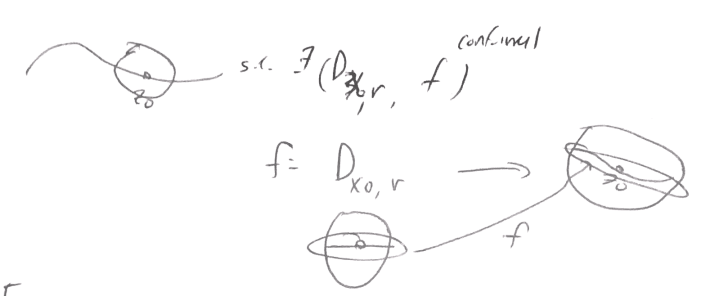
\includegraphics[width=.8\textwidth]{Figures/curve.png}}\]
     For all $z_0 \in \Gamma$, there exist some neighborhood $N$ around $z_0$ and $(D_{x_0, r}, f)$ such that $f$ maps the diameter of $D_{x_0, r}$ to $N \cap \gamma$.
\end{definition}

\begin{example}
    The ellipse $\frac{x^2}{a^2} + \frac{y^2}{b^2} = 1$ is an analytic curve.
\end{example}

The main idea behind reflection across analytic curves is as follows:\\\\
Suppose $\Omega$ is some domain where $\partial \Omega$ is an analytic curve:
\[\fbox{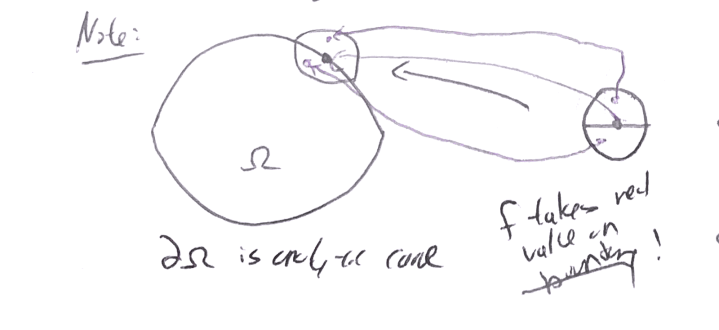
\includegraphics[width=.8\textwidth]{Figures/extension.png}}\]
The symmetry in the disk induces a symmetry near $\partial \Omega$, so we can extend it locally and use the reflection principle.

\begin{proposition}
Harmonic functions are real-analytic, meaning that the function is locally representable in power series as
\[(x - x_0)^n \cdot (y - y_0)^m\]
Or equivalently as power-series:
\[(z - z_0)^k (\overline{z - z_0})^\ell\]
\end{proposition}

\begin{proof}
    Recall the Poisson Formula lets you write a harmonic function $u(z)$ as
    \[u(z) = \int_{\mathbb{T}} f(\xi) \frac{d\xi}{2\pi} + \sum_{k > 0} z^k \int f(\xi) \overline{\xi}^k \frac{|d\xi|}{2\pi} + \sum_{k > 0} \overline{z}^k \int f(\xi) \xi^k \frac{|d\xi|}{2\pi}\]
    Applying a change of coordinates, we can reconstruct the power series based on harmonic values od disks.
\end{proof}

\section{Lecture - 11/16/2022}

\subsection{Harmonic Conjugates}

\begin{definition}
    Let $\Omega$ be a domain and real-valued $u \in \text{Harm}(\Omega)$, suppose there exist real-valued $v \in \text{Harm}(\Omega)$ such that
    \[u + iv \in \text{Hol}(\Omega)\]
    then $v$ is called the \textbf{harmonic conjugate} of $u$ and we denote $\Tilde{u} \coloneqq v$. In particular, note that $\Tilde{v} = -u$. Note that all complex conjugates of $u$ \underline{differ by a constant}.
\end{definition}

\begin{theorem}
    If $\Omega$ is a simply connected domain, then harmonic conjugates always exist.
\end{theorem}

\begin{proof}
    Let $u \in \text{Harm}(\Omega)$, then by the Cauchy-Riemann Equation, it suffices to find $v \in \text{Harm}(\Omega)$ satisfying:
    \[\frac{\partial u}{\partial x} = \frac{\partial v}{\partial y}, \frac{\partial u}{\partial y} = -\frac{\partial u}{\partial x}\]
    Or equivalently that
    \[dv = \frac{\partial v}{\partial x} dx + \frac{\partial v}{\partial y} dy = - \frac{\partial u}{\partial y} dx + \frac{\partial u}{\partial x} dy\]
    Now fix $z_0 \in \Omega$, then we claim that
    \[v(\xi) = a + \int_{z_0}^\xi - \frac{\partial u}{\partial y} dx + \frac{\partial u}{\partial x} dy\]
    is our desired function. Note that $v$ is well-defined since $\Omega$ is simply connected. Now clearly $u + iv$ is holomorphic, so it remains for us to show that $v$ is harmonic:
    \begin{align*}
        d(dv) &= d(- \frac{\partial u}{\partial y} dx + \frac{\partial u}{\partial x} dy)\\
        &= -\frac{\partial^2 u}{\partial y^2} dy \wedge dx + \frac{\partial^2 u}{\partial x^2} dx \wedge dy\\
        &= (\Delta u) dx \wedge dy\\
        &= 0 \tag*{$u$ is harmonic}
    \end{align*}
\end{proof}

\begin{remark}
    The assumption that $\Omega$ is simply connected is essential. Consider the following example:
    \[u(z) = \ln |z| \text{ on } r < |z| < R\]
    We claim that $u$ does not have any harmonic conjugates.
\end{remark}

\begin{proof}
Suppose a conjugate $v$ does exist, then
\[dv = - \frac{\partial u}{\partial y} dx + \frac{\partial u}{\partial x} dy\]
Let $r'$ be between $r$ and $R$ and $C_{r'}$ be the circle centered at origin of radius $r'$, since $C_{r'}$ is a closed loop, endpoints match, so
\[\int_{C_{r'}} - \frac{\partial u}{\partial y} dx + \frac{\partial u}{\partial x} dy = 0\]
However, evaluating the integral explicitly gives us that 
\[- \frac{\partial u}{\partial y} dx + \frac{\partial u}{\partial x} dy \neq 0\]
\end{proof}

\begin{question}
    Let $\Dbb$ be the unit disk. Suppose $u \in \text{Harm}(\Dbb) \cap C(\overline{\Dbb}^{cl})$, then we know $u$ contains a harmonic conjugate $v$. How can we describe $u + iv$ explicitly?
\end{question}

\begin{proof}[Idea]
The idea is to find $S(z) \in \text{Hol}(\Dbb)$ such that
\[P(z) = \text{Re}(S(z))\]
, where $P(z)$ is the Poisson Formula. Then we have that
\[f(z) = \int_{\Tbb} S(z \overline{\xi}) u(\xi) \frac{|d\xi|}{2\pi}\]
Note that $f$ is analytic by Morera's Theorem and
\[\text{Re}(f(z)) = \int_{\Tbb} P(z \overline{\xi}) u(\xi) \frac{|d\xi|}{2\pi} = u(\xi)\]
So, how do we find this desired $S(z)$? Recall that
\[P(z) = 1 + \sum_{k \geq 1} z^k + \sum_{k \geq 1} \overline{z}^k\]
Then choosing
\begin{align*}
    S(z) &\coloneqq 1 + 2 \sum_{k \geq 1} z^k\\
    &= 1 + \frac{2z}{1 - z} \tag*{Domain of $S(z)$ is $\Dbb$}\\
    &= \frac{1 + z}{1 - z}
\end{align*}
will suffice. $S(z)$ is sometimes called the \textbf{Schwartz Kernel}.\\\\
Now let $Q(z) = \text{Im}(S(z))$, then
\[v(z) = \text{Im}(f(z)) = \int_{\Tbb} Q(z \xi) u(\xi) \frac{|d\xi|}{2\pi}\]
So we have that
\begin{align*}
    f(z) &= u(z) + i v(z)\\
    &= \int_{\Tbb} u(\xi) \frac{1 + z \overline{\xi}}{1 - z \overline{\xi}} \frac{|d\xi|}{2\pi}\\
    &= \int_{\Tbb} u(\xi) \frac{\xi + z}{\xi - z} \frac{|d\xi|}{2\pi}
\end{align*}
\end{proof}

\subsection{Reflection Principle for Analytic Functions}

Let $\Omega = \Omega^*$ be a symmetric domain and $f \in \text{Hol}(\Omega^+)$ such that
\[\lim_{z \to \xi} \text{Im}(f(z)) = 0,\ \forall \xi \in \Rbb \cap \Omega\]
(recall previously we assumed that the limit to the real part exists) 

Let $f = u + iv$. Recall the reflection principle allowed us to extend $v$ harmonically to
\[\Tilde{v}(z) = \begin{cases}
    v(z),\ z \in \Omega^+\\
    0,\ z \in \Rbb \cap \Omega\\
    -u(\overline{z}),\ z \in \Omega^-
\end{cases}\]

We can extend u to $\Tilde{u}$ on $\Omega \setminus \Rbb$ as
\[\Tilde{u}(z) = \begin{cases}
    u(z),\ z \in \Omega^+\\
    u(\overline{z}),\ z \in \Omega^-
\end{cases}\]

Altogether, this extends $f$ to a function $\Tilde{f} \in \text{Hol}(\Omega \setminus \Rbb)$.\\

For a particular $\xi_0 \in \Rbb$, consider the diagram:
\[\fbox{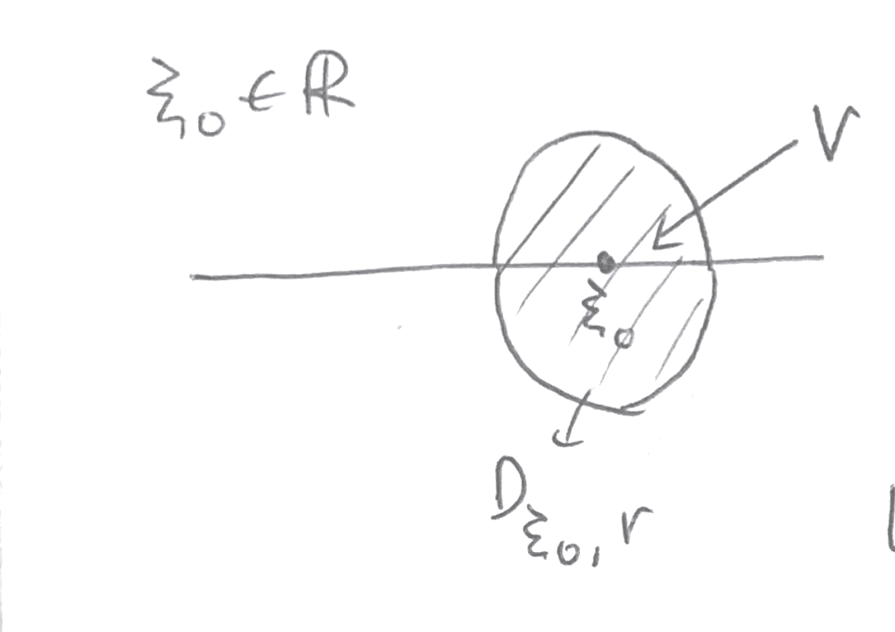
\includegraphics[width=.8\textwidth]{Figures/reflection_pricp.png}}\]

Let $u, v$ be harmonic on the upper-half disk as before, and let $\Tilde{v}$ be the extension of $v$ and $v'$ be the harmonic conjugate, then
\[-v' + i\Tilde{v} \in \text{Hol}(D_{\xi_0, r})\]

We can choose $v'$ to be symmetric ($v'(z) = v'(\overline{z})$ (Follows from the Schwartz Kernel Formula), then it follows that
\[-v'(z) = u(z) + C, \forall z \in D_{\xi_0, r}^+\]

\subsection{Liouville's Theorem for Harmonic Functions}

\begin{theorem}[Liouville's Theorem for Harmonic Functions]
    Let $u \in \text{Harm}(\Cbb)$, if for all $z \in \Cbb$, $|u(z)| \leq C < \infty$, then $u(z)$ is identically constant.
\end{theorem}

The proof of this theorem relies on the following lemma:

\begin{theorem}[Harnack's Inequality]
    If $u \in \text{Harm}(D_{0, R})$ and $u \geq 0$ is non-negative, then for any $|z| \leq r < R$,
    \[\frac{R - r}{R + r} u(0) \leq u(z) \leq \frac{R + r}{R - r} u(0)\]
\end{theorem}

\begin{proof}[Proof of Harnack's Inequality]
    If $R = 1$, then consider $u \in \text{Harm}(\Dbb) \cap C(\overline{D}^{cl})$, then we can write
    \[u(z) = \int_{\Tbb} \frac{1 - |z \overline{\xi}|^2}{|1 - z \xi|^2} u(\xi) \frac{|d\xi|}{2\pi}\]
    , where we know that $\xi$ takes values from $\Tbb$ the unit circle, so
    \begin{align*}
        \frac{1 - |z \overline{\xi}|^2}{|1 - z \xi|^2} &\leq \frac{(1 - |z|)(1 + |z|)}{(1 - |z|)^2}\\
        &= \frac{1 + |z|}{1 - |z|}\\
        &\leq \frac{1 + r}{1 - r} \tag*{Since $|z|$ is monotonic}
        \frac{1 - |z \overline{\xi}|^2}{|1 - z \xi|^2} &\geq \frac{(1 - |z|)(1 + |z|)}{(1 + |z|)^2}\\
        &= \frac{1 - |z|}{1 + |z|}\\
        &\geq \frac{1 - r}{1 + r} \tag*{Since $|z|$ is monotonic}
    \end{align*}
    So we have the inequality
    \[\frac{R - 1}{R + 1} u(0) \leq u(z) \leq \frac{R + 1}{R - 1} u(0)\]
    Now for a general $R$, consider
    \[u_a(z) = u(az), a < R\]
    Then we will eventually get the inequality that
    \[\frac{a - r}{a + r} u(0) \leq u(z) \leq \frac{a + r}{a - r} u(0)\]
    Then we can take the limit as $a \to R$.
\end{proof}

Now we are ready to prove Liouville's Theorem for Harmonic Functions:

\begin{proof}
    Let $|z| \leq r$, we can without loss replace $u$ by $u + C$ so that $u$ is non-negative (we can do this because $u$ is bounded). So Harnack's Inequality gives us that
    \[\frac{R - r}{R + r} u(0) \leq u(z) \leq \frac{R + r}{R - r} u(0)\]
    Taking $r \to \infty$ on both sides gives us that
    \[u(0) \leq u(z) \leq u(0),\ \forall z \in \Cbb\]
\end{proof}

\section{Lecture - 12/5/2022}

\subsection{Common Mistakes on Midterm}

You are allowed to resubmit for the midterm! Please either send an email with the resubmitted programs or send a regrade request on Gradescope. Midterm Resubmission to due this Friday by \textbf{midnight}.\\

There were two common mistakes a lot of people had on the midterm:
\begin{enumerate}
    \item \textbf{Hyperbolic Disks: } There were some confusions on finding the Euclidean center of the disk. The idea is to first solve the question in the case where the hyperbolic center is $a = 0$:
    \[\fbox{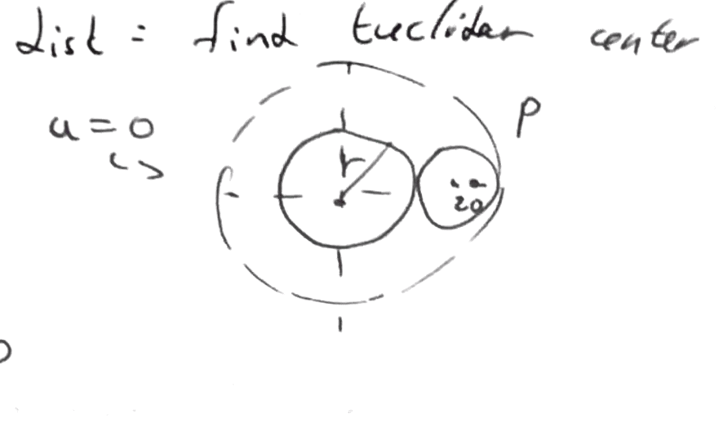
\includegraphics[width=.5\textwidth]{Figures/hyperbolic.png}}\]
    When $a = 0$, we have that
    \[\rho = \ln (\frac{1 + r}{1 - r})\]
    , and the Euclidean center coincide with the hyperbolic center. Now consider when $a = z_0$, then the following Mobius Transformation:
    \[z \mapsto \frac{z - z_0}{1 - \overline{z_0}z}\]
    maps hyperbolic disk to hyperbolic disk at the center. But note that $z_0$ is not the Euclidean center of its disks!\\\\
    It remains for us to find the Euclidean center of the disk, there are two ways to do this:
    \begin{itemize}
        \item Find $2$ points on the diameter opposite to each other
        \item Linear Fractional Transformation preserves symmetry, so Euclidean centers are symmetric to $\infty$, then we can find the inverse image of infinity, abd this map goes to $\frac{1}{\overline{z_0}}$
    \end{itemize}
    \item $f^N\ $ analytic \implies $f$ analytic: The common approach is first fix $z_0$ and write
    \[f(z)^N - f(z_0)^N = (f(z) - f(z_0)) \cdot (....)\]
    Then the claim is that if $f(z_0) \neq 0$, then $f(z)^N - f(z_0)^N$ be differentiable gives differentiability on $f(z) - f(z_0)$.\\\\
    In the case where $f(z_0) = 0$, we prove that the roots of $f$ are isolated and are in fact removable singularities.\\\\
    \textbf{There's another approach to this: }
    Let $U$ be some domain around $z_0$ small enough, then the $N$-th root of $z_0$ creates exactly $N$ regions whose $N$-th power goes to $U$:
    \[\fbox{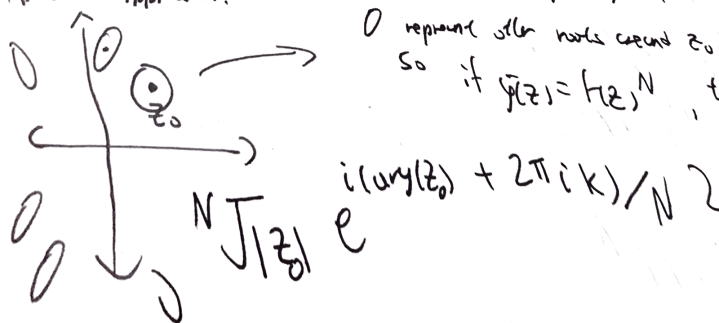
\includegraphics[width=.5\textwidth]{Figures/root.png}}\]
    In other words, if $g(z) = f(z)^N$, there exist analytic branches of $f(z) = g(z)^{1/N}$. We then claim that $f(z)$ must be in exactly ONE of these branches!\\\\
    This claim follows from the fact that each branch is connected, $f$ is continuous, and the continuous image of $f$ has to be connected.
\end{enumerate}

\subsection{Analytic Continuation}

Previously we have seen that functions like $\sqrt{1 - z^2}, \log(z)$ are not well-defined on the complex plane, as they are multi-valued functions. However, there's a way to make them well-defined by representing them on \textbf{Riemann surfaces} instead.\\

One notion to introduce Riemann Surfaces uses the idea of Analytic Continuation.\\

There's a naive approach to analytic continuation. Let $f \in Hol(\Omega)$ and consider some $z_0 \in \Omega$ as follows:
\[\fbox{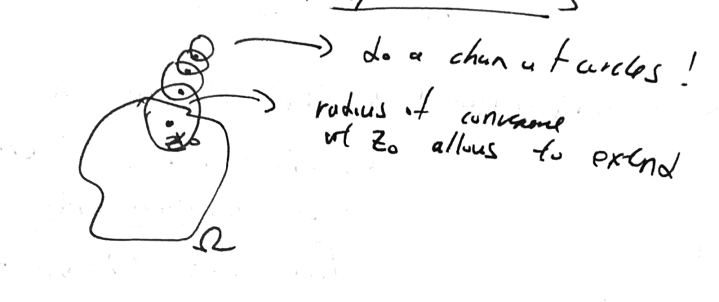
\includegraphics[width=.6\textwidth]{Figures/chain_circles.png}}\]
The idea is if the local power series at $z_0$ has radius of convergence greater than $d(z_0, \partial \Omega)$, then we could extend $f$ out of $\Omega$. If we can repeatedly do this, we can construct a chain of balls out of the boundary.\\

However, there are two problems with this approach:
\begin{enumerate}
    \item You are not always guaranteed that you can construct this chain of balls.
    \item Sometimes your extension may not match up with one another. For example take $f = \sqrt{z}$ with $\Omega$ being on the right half-plane:
    \[\fbox{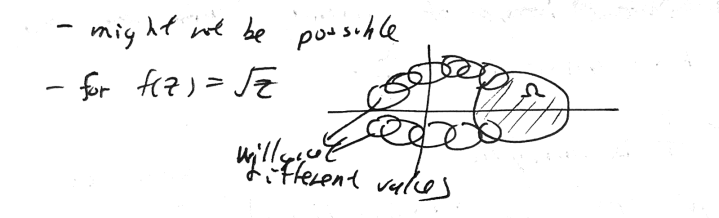
\includegraphics[width=.6\textwidth]{Figures/chain_root.png}}\]
    If you take a chain of circles going from the clock-wise and counter-clockwise direction, they WILL not give the same value when they meet.
\end{enumerate}

Therefore, we need a more standard way to discuss analytic continuation, and this leads to the idea of analytic continuation along a path.

\begin{definition}[Analytic Continuation Along a Path]
    Let $\gamma: [a, b] \to \Cbb$ be a path, we say that an \textbf{analytic continuation exists along $\gamma$} if there exist a family of $(f_s, U_s)$, $s \in [a, b]$ such that
    \[\gamma(s) \in U_s, f_s \in \text{Hol}(U_s)\]
    and for all $t_0 \in [a, b]$, there exist $\delta > 0$ such that
    \[|t - t_0| < \delta \implies \begin{cases}
    1.\ U_t \cap U_{t_0} \neq \emptyset\\
    2.\ f_t \equiv f_{t_0} \text{ on } U_t \cap U_{t_0}
    \end{cases}\]
\end{definition}

\begin{remark}
    In practice, once we have the family of functions, we will simplify $f_t$ as
    \[f_t(z) = \sum_0^\infty a_k(t) (z - \gamma(t))^k\]
    as a power series and take $U_t$ as a disk instead.
\end{remark}

\begin{proposition}
    Let $\gamma: [a, b] \to \Cbb$ be a path, an \textbf{analytic continuation exists along $\gamma$} if and only if there exists a finite division of $[a, b]$ into intervals $I_1, ..., I_n$ and family $(f_i, U_i)_{i = 1}^n$ such that
    \begin{itemize}
        \item $\gamma(I_k) \subseteq U_k$
        \item $U_k \cap U_{k+1} \neq \emptyset$
        \item $f_k \equiv f_{k+1}$ on $U_k \cap U_{k+1}$
    \end{itemize}
\end{proposition}

\begin{proof}
    Converse is straight-forward, for all $t \in [a, b]$, just choose $g_t$ to be $f_k$ if $t \in I_k$, then we have $(g_t, U_t)$ to be a valid family.\\\\
    For the forward, direction, consider $U_t$ for each $t \in [a, b]$ and
    \[\bigcup_{t \in [a, b]} \gamma^{-1}(U_t) \text{ is a cover of } [a, b]\]
    Then the Lebesgue Number's Lemma implies that there exists some $\alpha > 0$ such that for any $E \subseteq [a, b]$ where $diam(E) < \alpha$, there exist $U_t$ such that $E \subset \varphi^{-1}(U_t)$.\\\\
    Then we split intervals of $[a, b]$ to intervals $I_1, ..., I_n$ each less than $\alpha$ in length. Then for $I_k = [a_{k-1}, a_k]$ we have that $I_k \subseteq \gamma^{-1}(U_{t_k})$, hence $\gamma(I_k) \subseteq U_{t_k}$.\\\\
    Then the family $(f_{t_k}, U_{t_k})$ is our desired finite division.
\end{proof}

\begin{proposition}
    Analytic Continuation along a path is independent of the choice of splitting. In other words, the analytic continuation is unique.
\end{proposition}

\begin{proof}
    This follows from the Uniquenss Theorem of analytic functions. Suppose we have a finite splitting ${I_k}, {J_j}$ of $[a, b]$, then we can consider the splitting $\{I_k \cap I_j\}$ of $[a, b]$. This is a finer splitting than both given, then we apply the Uniqueness Theorem.
\end{proof}

\begin{definition}[Germs of Analytic Functions]
    Let $z_0 \in \Cbb$, then this consider the set of the form:
    \[S = \{(f, U)\ |\ \text{$f \in \text{Hol}(U)$, $U$ is a neighborhod of $z_0$}\}\]
    We can define an equivalence relation as follows, where $(f, U) \sim (g, V)$ if there exists some neighborhood $W \subseteq U \cap V$ containing $z_0$ such that $f \equiv g$ on $W$.\\\\
    This equivalence class is called the \textbf{germ of analytic functions at $z_0$}, which we denote an element of this class as $[f]_{z_0}$ and call it the \textbf{germ of $f$ at $z_0$}.
\end{definition}

\begin{remark}
    If $U, V$ are connected and convex domains, we can without loss take $W = U \cap V$. Analytic continuation being unique is essentially saying that our germs coincides along the path.
\end{remark}

\subsection{Monodromy's Theorem}
\begin{theorem}[Monodromy's Theorem]
    Suppose $\gamma_0, \gamma_1: [a, b] \to \Cbb$ are homotopy pathes with same start and end points, meaning there exist a continuous function $\Gamma(t, s): [a, b] \to [0, 1] \to \Cbb$ such that
    \[\Gamma(t, 0) = \gamma_0(t), \Gamma(t, 1) = \gamma_1(t), \Gamma(a, s) = z_0, \Gamma(b, s) = z_1\]
    Define $\gamma_s(t) \coloneqq \Gamma(t, s)$ for all $s \in [a, b]$. Suppose there exists analytic continuation along all of $\gamma_s(t)$ for some analytic function $f$, then the analytic continuation of $[f]_{\gamma_s(b)}$ is independent on $s$!
\end{theorem}

\begin{proof}[Idea]
    If two analytic continuations are ``close enough", they are the same.
\end{proof}

\begin{example}
    Take $f = \sqrt{z}$ on the principle branch, consider the two following ways to draw pathes from $\gamma_0(a) = 1$ to $\gamma_0(b) = -1$:
    \[\fbox{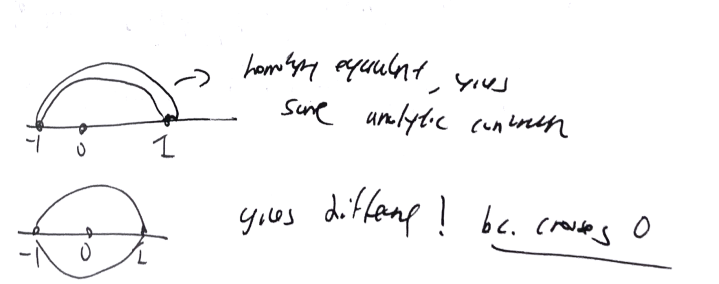
\includegraphics[width=.6\textwidth]{Figures/sqrt_root.png}}\]
    The pathes in the top figure are homotopy equivalent, the pathes in the bottom figure are not.
\end{example}

\end{document}
